
\section{Results and Analysis}
\label{sec:evaluation}
\subsection{Effectiveness of Rankers with Different Query Agents}
\label{sec:effectiveness-experiment}

\subsubsection{Setup}
\section{Method}\label{sec:method}
\begin{figure}
    \centering
    \includegraphics[width=0.85\textwidth]{imgs/heatmap_acc.pdf}
    \caption{\textbf{Visualization of the proposed periodic Bayesian flow with mean parameter $\mu$ and accumulated accuracy parameter $c$ which corresponds to the entropy/uncertainty}. For $x = 0.3, \beta(1) = 1000$ and $\alpha_i$ defined in \cref{appd:bfn_cir}, this figure plots three colored stochastic parameter trajectories for receiver mean parameter $m$ and accumulated accuracy parameter $c$, superimposed on a log-scale heatmap of the Bayesian flow distribution $p_F(m|x,\senderacc)$ and $p_F(c|x,\senderacc)$. Note the \emph{non-monotonicity} and \emph{non-additive} property of $c$ which could inform the network the entropy of the mean parameter $m$ as a condition and the \emph{periodicity} of $m$. %\jj{Shrink the figures to save space}\hanlin{Do we need to make this figure one-column?}
    }
    \label{fig:vmbf_vis}
    \vskip -0.1in
\end{figure}
% \begin{wrapfigure}{r}{0.5\textwidth}
%     \centering
%     \includegraphics[width=0.49\textwidth]{imgs/heatmap_acc.pdf}
%     \caption{\textbf{Visualization of hyper-torus Bayesian flow based on von Mises Distribution}. For $x = 0.3, \beta(1) = 1000$ and $\alpha_i$ defined in \cref{appd:bfn_cir}, this figure plots three colored stochastic parameter trajectories for receiver mean parameter $m$ and accumulated accuracy parameter $c$, superimposed on a log-scale heatmap of the Bayesian flow distribution $p_F(m|x,\senderacc)$ and $p_F(c|x,\senderacc)$. Note the \emph{non-monotonicity} and \emph{non-additive} property of $c$. \jj{Shrink the figures to save space}}
%     \label{fig:vmbf_vis}
%     \vspace{-30pt}
% \end{wrapfigure}


In this section, we explain the detailed design of CrysBFN tackling theoretical and practical challenges. First, we describe how to derive our new formulation of Bayesian Flow Networks over hyper-torus $\mathbb{T}^{D}$ from scratch. Next, we illustrate the two key differences between \modelname and the original form of BFN: $1)$ a meticulously designed novel base distribution with different Bayesian update rules; and $2)$ different properties over the accuracy scheduling resulted from the periodicity and the new Bayesian update rules. Then, we present in detail the overall framework of \modelname over each manifold of the crystal space (\textit{i.e.} fractional coordinates, lattice vectors, atom types) respecting \textit{periodic E(3) invariance}. 

% In this section, we first demonstrate how to build Bayesian flow on hyper-torus $\mathbb{T}^{D}$ by overcoming theoretical and practical problems to provide a low-noise parameter-space approach to fractional atom coordinate generation. Next, we present how \modelname models each manifold of crystal space respecting \textit{periodic E(3) invariance}. 

\subsection{Periodic Bayesian Flow on Hyper-torus \texorpdfstring{$\mathbb{T}^{D}$}{}} 
For generative modeling of fractional coordinates in crystal, we first construct a periodic Bayesian flow on \texorpdfstring{$\mathbb{T}^{D}$}{} by designing every component of the totally new Bayesian update process which we demonstrate to be distinct from the original Bayesian flow (please see \cref{fig:non_add}). 
 %:) 
 
 The fractional atom coordinate system \citep{jiao2023crystal} inherently distributes over a hyper-torus support $\mathbb{T}^{3\times N}$. Hence, the normal distribution support on $\R$ used in the original \citep{bfn} is not suitable for this scenario. 
% The key problem of generative modeling for crystal is the periodicity of Cartesian atom coordinates $\vX$ requiring:
% \begin{equation}\label{eq:periodcity}
% p(\vA,\vL,\vX)=p(\vA,\vL,\vX+\vec{LK}),\text{where}~\vec{K}=\vec{k}\vec{1}_{1\times N},\forall\vec{k}\in\mathbb{Z}^{3\times1}
% \end{equation}
% However, there does not exist such a distribution supporting on $\R$ to model such property because the integration of such distribution over $\R$ will not be finite and equal to 1. Therefore, the normal distribution used in \citet{bfn} can not meet this condition.

To tackle this problem, the circular distribution~\citep{mardia2009directional} over the finite interval $[-\pi,\pi)$ is a natural choice as the base distribution for deriving the BFN on $\mathbb{T}^D$. 
% one natural choice is to 
% we would like to consider the circular distribution over the finite interval as the base 
% we find that circular distributions \citep{mardia2009directional} defined on a finite interval with lengths of $2\pi$ can be used as the instantiation of input distribution for the BFN on $\mathbb{T}^D$.
Specifically, circular distributions enjoy desirable periodic properties: $1)$ the integration over any interval length of $2\pi$ equals 1; $2)$ the probability distribution function is periodic with period $2\pi$.  Sharing the same intrinsic with fractional coordinates, such periodic property of circular distribution makes it suitable for the instantiation of BFN's input distribution, in parameterizing the belief towards ground truth $\x$ on $\mathbb{T}^D$. 
% \yuxuan{this is very complicated from my perspective.} \hanlin{But this property is exactly beautiful and perfectly fit into the BFN.}

\textbf{von Mises Distribution and its Bayesian Update} We choose von Mises distribution \citep{mardia2009directional} from various circular distributions as the form of input distribution, based on the appealing conjugacy property required in the derivation of the BFN framework.
% to leverage the Bayesian conjugacy property of von Mises distribution which is required by the BFN framework. 
That is, the posterior of a von Mises distribution parameterized likelihood is still in the family of von Mises distributions. The probability density function of von Mises distribution with mean direction parameter $m$ and concentration parameter $c$ (describing the entropy/uncertainty of $m$) is defined as: 
\begin{equation}
f(x|m,c)=vM(x|m,c)=\frac{\exp(c\cos(x-m))}{2\pi I_0(c)}
\end{equation}
where $I_0(c)$ is zeroth order modified Bessel function of the first kind as the normalizing constant. Given the last univariate belief parameterized by von Mises distribution with parameter $\theta_{i-1}=\{m_{i-1},\ c_{i-1}\}$ and the sample $y$ from sender distribution with unknown data sample $x$ and known accuracy $\alpha$ describing the entropy/uncertainty of $y$,  Bayesian update for the receiver is deducted as:
\begin{equation}
 h(\{m_{i-1},c_{i-1}\},y,\alpha)=\{m_i,c_i \}, \text{where}
\end{equation}
\begin{equation}\label{eq:h_m}
m_i=\text{atan2}(\alpha\sin y+c_{i-1}\sin m_{i-1}, {\alpha\cos y+c_{i-1}\cos m_{i-1}})
\end{equation}
\begin{equation}\label{eq:h_c}
c_i =\sqrt{\alpha^2+c_{i-1}^2+2\alpha c_{i-1}\cos(y-m_{i-1})}
\end{equation}
The proof of the above equations can be found in \cref{apdx:bayesian_update_function}. The atan2 function refers to  2-argument arctangent. Independently conducting  Bayesian update for each dimension, we can obtain the Bayesian update distribution by marginalizing $\y$:
\begin{equation}
p_U(\vtheta'|\vtheta,\bold{x};\alpha)=\mathbb{E}_{p_S(\bold{y}|\bold{x};\alpha)}\delta(\vtheta'-h(\vtheta,\bold{y},\alpha))=\mathbb{E}_{vM(\bold{y}|\bold{x},\alpha)}\delta(\vtheta'-h(\vtheta,\bold{y},\alpha))
\end{equation} 
\begin{figure}
    \centering
    \vskip -0.15in
    \includegraphics[width=0.95\linewidth]{imgs/non_add.pdf}
    \caption{An intuitive illustration of non-additive accuracy Bayesian update on the torus. The lengths of arrows represent the uncertainty/entropy of the belief (\emph{e.g.}~$1/\sigma^2$ for Gaussian and $c$ for von Mises). The directions of the arrows represent the believed location (\emph{e.g.}~ $\mu$ for Gaussian and $m$ for von Mises).}
    \label{fig:non_add}
    \vskip -0.15in
\end{figure}
\textbf{Non-additive Accuracy} 
The additive accuracy is a nice property held with the Gaussian-formed sender distribution of the original BFN expressed as:
\begin{align}
\label{eq:standard_id}
    \update(\parsn{}'' \mid \parsn{}, \x; \alpha_a+\alpha_b) = \E_{\update(\parsn{}' \mid \parsn{}, \x; \alpha_a)} \update(\parsn{}'' \mid \parsn{}', \x; \alpha_b)
\end{align}
Such property is mainly derived based on the standard identity of Gaussian variable:
\begin{equation}
X \sim \mathcal{N}\left(\mu_X, \sigma_X^2\right), Y \sim \mathcal{N}\left(\mu_Y, \sigma_Y^2\right) \Longrightarrow X+Y \sim \mathcal{N}\left(\mu_X+\mu_Y, \sigma_X^2+\sigma_Y^2\right)
\end{equation}
The additive accuracy property makes it feasible to derive the Bayesian flow distribution $
p_F(\boldsymbol{\theta} \mid \mathbf{x} ; i)=p_U\left(\boldsymbol{\theta} \mid \boldsymbol{\theta}_0, \mathbf{x}, \sum_{k=1}^{i} \alpha_i \right)
$ for the simulation-free training of \cref{eq:loss_n}.
It should be noted that the standard identity in \cref{eq:standard_id} does not hold in the von Mises distribution. Hence there exists an important difference between the original Bayesian flow defined on Euclidean space and the Bayesian flow of circular data on $\mathbb{T}^D$ based on von Mises distribution. With prior $\btheta = \{\bold{0},\bold{0}\}$, we could formally represent the non-additive accuracy issue as:
% The additive accuracy property implies the fact that the "confidence" for the data sample after observing a series of the noisy samples with accuracy ${\alpha_1, \cdots, \alpha_i}$ could be  as the accuracy sum  which could be  
% Here we 
% Here we emphasize the specific property of BFN based on von Mises distribution.
% Note that 
% \begin{equation}
% \update(\parsn'' \mid \parsn, \x; \alpha_a+\alpha_b) \ne \E_{\update(\parsn' \mid \parsn, \x; \alpha_a)} \update(\parsn'' \mid \parsn', \x; \alpha_b)
% \end{equation}
% \oyyw{please check whether the below equation is better}
% \yuxuan{I fill somehow confusing on what is the update distribution with $\alpha$. }
% \begin{equation}
% \update(\parsn{}'' \mid \parsn{}, \x; \alpha_a+\alpha_b) \ne \E_{\update(\parsn{}' \mid \parsn{}, \x; \alpha_a)} \update(\parsn{}'' \mid \parsn{}', \x; \alpha_b)
% \end{equation}
% We give an intuitive visualization of such difference in \cref{fig:non_add}. The untenability of this property can materialize by considering the following case: with prior $\btheta = \{\bold{0},\bold{0}\}$, check the two-step Bayesian update distribution with $\alpha_a,\alpha_b$ and one-step Bayesian update with $\alpha=\alpha_a+\alpha_b$:
\begin{align}
\label{eq:nonadd}
     &\update(c'' \mid \parsn, \x; \alpha_a+\alpha_b)  = \delta(c-\alpha_a-\alpha_b)
     \ne  \mathbb{E}_{p_U(\parsn' \mid \parsn, \x; \alpha_a)}\update(c'' \mid \parsn', \x; \alpha_b) \nonumber \\&= \mathbb{E}_{vM(\bold{y}_b|\bold{x},\alpha_a)}\mathbb{E}_{vM(\bold{y}_a|\bold{x},\alpha_b)}\delta(c-||[\alpha_a \cos\y_a+\alpha_b\cos \y_b,\alpha_a \sin\y_a+\alpha_b\sin \y_b]^T||_2)
\end{align}
A more intuitive visualization could be found in \cref{fig:non_add}. This fundamental difference between periodic Bayesian flow and that of \citet{bfn} presents both theoretical and practical challenges, which we will explain and address in the following contents.

% This makes constructing Bayesian flow based on von Mises distribution intrinsically different from previous Bayesian flows (\citet{bfn}).

% Thus, we must reformulate the framework of Bayesian flow networks  accordingly. % and do necessary reformulations of BFN. 

% \yuxuan{overall I feel this part is complicated by using the language of update distribution. I would like to suggest simply use bayesian update, to provide intuitive explantion.}\hanlin{See the illustration in \cref{fig:non_add}}

% That introduces a cascade of problems, and we investigate the following issues: $(1)$ Accuracies between sender and receiver are not synchronized and need to be differentiated. $(2)$ There is no tractable Bayesian flow distribution for a one-step sample conditioned on a given time step $i$, and naively simulating the Bayesian flow results in computational overhead. $(3)$ It is difficult to control the entropy of the Bayesian flow. $(4)$ Accuracy is no longer a function of $t$ and becomes a distribution conditioned on $t$, which can be different across dimensions.
%\jj{Edited till here}

\textbf{Entropy Conditioning} As a common practice in generative models~\citep{ddpm,flowmatching,bfn}, timestep $t$ is widely used to distinguish among generation states by feeding the timestep information into the networks. However, this paper shows that for periodic Bayesian flow, the accumulated accuracy $\vc_i$ is more effective than time-based conditioning by informing the network about the entropy and certainty of the states $\parsnt{i}$. This stems from the intrinsic non-additive accuracy which makes the receiver's accumulated accuracy $c$ not bijective function of $t$, but a distribution conditioned on accumulated accuracies $\vc_i$ instead. Therefore, the entropy parameter $\vc$ is taken logarithm and fed into the network to describe the entropy of the input corrupted structure. We verify this consideration in \cref{sec:exp_ablation}. 
% \yuxuan{implement variant. traditionally, the timestep is widely used to distinguish the different states by putting the timestep embedding into the networks. citation of FM, diffusion, BFN. However, we find that conditioned on time in periodic flow could not provide extra benefits. To further boost the performance, we introduce a simple yet effective modification term entropy conditional. This is based on that the accumulated accuracy which represents the current uncertainty or entropy could be a better indicator to distinguish different states. + Describe how you do this. }



\textbf{Reformulations of BFN}. Recall the original update function with Gaussian sender distribution, after receiving noisy samples $\y_1,\y_2,\dots,\y_i$ with accuracies $\senderacc$, the accumulated accuracies of the receiver side could be analytically obtained by the additive property and it is consistent with the sender side.
% Since observing sample $\y$ with $\alpha_i$ can not result in exact accuracy increment $\alpha_i$ for receiver, the accuracies between sender and receiver are not synchronized which need to be differentiated. 
However, as previously mentioned, this does not apply to periodic Bayesian flow, and some of the notations in original BFN~\citep{bfn} need to be adjusted accordingly. We maintain the notations of sender side's one-step accuracy $\alpha$ and added accuracy $\beta$, and alter the notation of receiver's accuracy parameter as $c$, which is needed to be simulated by cascade of Bayesian updates. We emphasize that the receiver's accumulated accuracy $c$ is no longer a function of $t$ (differently from the Gaussian case), and it becomes a distribution conditioned on received accuracies $\senderacc$ from the sender. Therefore, we represent the Bayesian flow distribution of von Mises distribution as $p_F(\btheta|\x;\alpha_1,\alpha_2,\dots,\alpha_i)$. And the original simulation-free training with Bayesian flow distribution is no longer applicable in this scenario.
% Different from previous BFNs where the accumulated accuracy $\rho$ is not explicitly modeled, the accumulated accuracy parameter $c$ (visualized in \cref{fig:vmbf_vis}) needs to be explicitly modeled by feeding it to the network to avoid information loss.
% the randomaccuracy parameter $c$ (visualized in \cref{fig:vmbf_vis}) implies that there exists information in $c$ from the sender just like $m$, meaning that $c$ also should be fed into the network to avoid information loss. 
% We ablate this consideration in  \cref{sec:exp_ablation}. 

\textbf{Fast Sampling from Equivalent Bayesian Flow Distribution} Based on the above reformulations, the Bayesian flow distribution of von Mises distribution is reframed as: 
\begin{equation}\label{eq:flow_frac}
p_F(\btheta_i|\x;\alpha_1,\alpha_2,\dots,\alpha_i)=\E_{\update(\parsnt{1} \mid \parsnt{0}, \x ; \alphat{1})}\dots\E_{\update(\parsn_{i-1} \mid \parsnt{i-2}, \x; \alphat{i-1})} \update(\parsnt{i} | \parsnt{i-1},\x;\alphat{i} )
\end{equation}
Naively sampling from \cref{eq:flow_frac} requires slow auto-regressive iterated simulation, making training unaffordable. Noticing the mathematical properties of \cref{eq:h_m,eq:h_c}, we  transform \cref{eq:flow_frac} to the equivalent form:
\begin{equation}\label{eq:cirflow_equiv}
p_F(\vec{m}_i|\x;\alpha_1,\alpha_2,\dots,\alpha_i)=\E_{vM(\y_1|\x,\alpha_1)\dots vM(\y_i|\x,\alpha_i)} \delta(\vec{m}_i-\text{atan2}(\sum_{j=1}^i \alpha_j \cos \y_j,\sum_{j=1}^i \alpha_j \sin \y_j))
\end{equation}
\begin{equation}\label{eq:cirflow_equiv2}
p_F(\vec{c}_i|\x;\alpha_1,\alpha_2,\dots,\alpha_i)=\E_{vM(\y_1|\x,\alpha_1)\dots vM(\y_i|\x,\alpha_i)}  \delta(\vec{c}_i-||[\sum_{j=1}^i \alpha_j \cos \y_j,\sum_{j=1}^i \alpha_j \sin \y_j]^T||_2)
\end{equation}
which bypasses the computation of intermediate variables and allows pure tensor operations, with negligible computational overhead.
\begin{restatable}{proposition}{cirflowequiv}
The probability density function of Bayesian flow distribution defined by \cref{eq:cirflow_equiv,eq:cirflow_equiv2} is equivalent to the original definition in \cref{eq:flow_frac}. 
\end{restatable}
\textbf{Numerical Determination of Linear Entropy Sender Accuracy Schedule} ~Original BFN designs the accuracy schedule $\beta(t)$ to make the entropy of input distribution linearly decrease. As for crystal generation task, to ensure information coherence between modalities, we choose a sender accuracy schedule $\senderacc$ that makes the receiver's belief entropy $H(t_i)=H(p_I(\cdot|\vtheta_i))=H(p_I(\cdot|\vc_i))$ linearly decrease \emph{w.r.t.} time $t_i$, given the initial and final accuracy parameter $c(0)$ and $c(1)$. Due to the intractability of \cref{eq:vm_entropy}, we first use numerical binary search in $[0,c(1)]$ to determine the receiver's $c(t_i)$ for $i=1,\dots, n$ by solving the equation $H(c(t_i))=(1-t_i)H(c(0))+tH(c(1))$. Next, with $c(t_i)$, we conduct numerical binary search for each $\alpha_i$ in $[0,c(1)]$ by solving the equations $\E_{y\sim vM(x,\alpha_i)}[\sqrt{\alpha_i^2+c_{i-1}^2+2\alpha_i c_{i-1}\cos(y-m_{i-1})}]=c(t_i)$ from $i=1$ to $i=n$ for arbitrarily selected $x\in[-\pi,\pi)$.

After tackling all those issues, we have now arrived at a new BFN architecture for effectively modeling crystals. Such BFN can also be adapted to other type of data located in hyper-torus $\mathbb{T}^{D}$.

\subsection{Equivariant Bayesian Flow for Crystal}
With the above Bayesian flow designed for generative modeling of fractional coordinate $\vF$, we are able to build equivariant Bayesian flow for each modality of crystal. In this section, we first give an overview of the general training and sampling algorithm of \modelname (visualized in \cref{fig:framework}). Then, we describe the details of the Bayesian flow of every modality. The training and sampling algorithm can be found in \cref{alg:train} and \cref{alg:sampling}.

\textbf{Overview} Operating in the parameter space $\bthetaM=\{\bthetaA,\bthetaL,\bthetaF\}$, \modelname generates high-fidelity crystals through a joint BFN sampling process on the parameter of  atom type $\bthetaA$, lattice parameter $\vec{\theta}^L=\{\bmuL,\brhoL\}$, and the parameter of fractional coordinate matrix $\bthetaF=\{\bmF,\bcF\}$. We index the $n$-steps of the generation process in a discrete manner $i$, and denote the corresponding continuous notation $t_i=i/n$ from prior parameter $\thetaM_0$ to a considerably low variance parameter $\thetaM_n$ (\emph{i.e.} large $\vrho^L,\bmF$, and centered $\bthetaA$).

At training time, \modelname samples time $i\sim U\{1,n\}$ and $\bthetaM_{i-1}$ from the Bayesian flow distribution of each modality, serving as the input to the network. The network $\net$ outputs $\net(\parsnt{i-1}^\mathcal{M},t_{i-1})=\net(\parsnt{i-1}^A,\parsnt{i-1}^F,\parsnt{i-1}^L,t_{i-1})$ and conducts gradient descents on loss function \cref{eq:loss_n} for each modality. After proper training, the sender distribution $p_S$ can be approximated by the receiver distribution $p_R$. 

At inference time, from predefined $\thetaM_0$, we conduct transitions from $\thetaM_{i-1}$ to $\thetaM_{i}$ by: $(1)$ sampling $\y_i\sim p_R(\bold{y}|\thetaM_{i-1};t_i,\alpha_i)$ according to network prediction $\predM{i-1}$; and $(2)$ performing Bayesian update $h(\thetaM_{i-1},\y^\calM_{i-1},\alpha_i)$ for each dimension. 

% Alternatively, we complete this transition using the flow-back technique by sampling 
% $\thetaM_{i}$ from Bayesian flow distribution $\flow(\btheta^M_{i}|\predM{i-1};t_{i-1})$. 

% The training objective of $\net$ is to minimize the KL divergence between sender distribution and receiver distribution for every modality as defined in \cref{eq:loss_n} which is equivalent to optimizing the negative variational lower bound $\calL^{VLB}$ as discussed in \cref{sec:preliminaries}. 

%In the following part, we will present the Bayesian flow of each modality in detail.

\textbf{Bayesian Flow of Fractional Coordinate $\vF$}~The distribution of the prior parameter $\bthetaF_0$ is defined as:
\begin{equation}\label{eq:prior_frac}
    p(\bthetaF_0) \defeq \{vM(\vm_0^F|\vec{0}_{3\times N},\vec{0}_{3\times N}),\delta(\vc_0^F-\vec{0}_{3\times N})\} = \{U(\vec{0},\vec{1}),\delta(\vc_0^F-\vec{0}_{3\times N})\}
\end{equation}
Note that this prior distribution of $\vm_0^F$ is uniform over $[\vec{0},\vec{1})$, ensuring the periodic translation invariance property in \cref{De:pi}. The training objective is minimizing the KL divergence between sender and receiver distribution (deduction can be found in \cref{appd:cir_loss}): 
%\oyyw{replace $\vF$ with $\x$?} \hanlin{notations follow Preliminary?}
\begin{align}\label{loss_frac}
\calL_F = n \E_{i \sim \ui{n}, \flow(\parsn{}^F \mid \vF ; \senderacc)} \alpha_i\frac{I_1(\alpha_i)}{I_0(\alpha_i)}(1-\cos(\vF-\predF{i-1}))
\end{align}
where $I_0(x)$ and $I_1(x)$ are the zeroth and the first order of modified Bessel functions. The transition from $\bthetaF_{i-1}$ to $\bthetaF_{i}$ is the Bayesian update distribution based on network prediction:
\begin{equation}\label{eq:transi_frac}
    p(\btheta^F_{i}|\parsnt{i-1}^\calM)=\mathbb{E}_{vM(\bold{y}|\predF{i-1},\alpha_i)}\delta(\btheta^F_{i}-h(\btheta^F_{i-1},\bold{y},\alpha_i))
\end{equation}
\begin{restatable}{proposition}{fracinv}
With $\net_{F}$ as a periodic translation equivariant function namely $\net_F(\parsnt{}^A,w(\parsnt{}^F+\vt),\parsnt{}^L,t)=w(\net_F(\parsnt{}^A,\parsnt{}^F,\parsnt{}^L,t)+\vt), \forall\vt\in\R^3$, the marginal distribution of $p(\vF_n)$ defined by \cref{eq:prior_frac,eq:transi_frac} is periodic translation invariant. 
\end{restatable}
\textbf{Bayesian Flow of Lattice Parameter \texorpdfstring{$\boldsymbol{L}$}{}}   
Noting the lattice parameter $\bm{L}$ located in Euclidean space, we set prior as the parameter of a isotropic multivariate normal distribution $\btheta^L_0\defeq\{\vmu_0^L,\vrho_0^L\}=\{\bm{0}_{3\times3},\bm{1}_{3\times3}\}$
% \begin{equation}\label{eq:lattice_prior}
% \btheta^L_0\defeq\{\vmu_0^L,\vrho_0^L\}=\{\bm{0}_{3\times3},\bm{1}_{3\times3}\}
% \end{equation}
such that the prior distribution of the Markov process on $\vmu^L$ is the Dirac distribution $\delta(\vec{\mu_0}-\vec{0})$ and $\delta(\vec{\rho_0}-\vec{1})$, 
% \begin{equation}
%     p_I^L(\boldsymbol{L}|\btheta_0^L)=\mathcal{N}(\bm{L}|\bm{0},\bm{I})
% \end{equation}
which ensures O(3)-invariance of prior distribution of $\vL$. By Eq. 77 from \citet{bfn}, the Bayesian flow distribution of the lattice parameter $\bm{L}$ is: 
\begin{align}% =p_U(\bmuL|\btheta_0^L,\bm{L},\beta(t))
p_F^L(\bmuL|\bm{L};t) &=\mathcal{N}(\bmuL|\gamma(t)\bm{L},\gamma(t)(1-\gamma(t))\bm{I}) 
\end{align}
where $\gamma(t) = 1 - \sigma_1^{2t}$ and $\sigma_1$ is the predefined hyper-parameter controlling the variance of input distribution at $t=1$ under linear entropy accuracy schedule. The variance parameter $\vrho$ does not need to be modeled and fed to the network, since it is deterministic given the accuracy schedule. After sampling $\bmuL_i$ from $p_F^L$, the training objective is defined as minimizing KL divergence between sender and receiver distribution (based on Eq. 96 in \citet{bfn}):
\begin{align}
\mathcal{L}_{L} = \frac{n}{2}\left(1-\sigma_1^{2/n}\right)\E_{i \sim \ui{n}}\E_{\flow(\bmuL_{i-1} |\vL ; t_{i-1})}  \frac{\left\|\vL -\predL{i-1}\right\|^2}{\sigma_1^{2i/n}},\label{eq:lattice_loss}
\end{align}
where the prediction term $\predL{i-1}$ is the lattice parameter part of network output. After training, the generation process is defined as the Bayesian update distribution given network prediction:
\begin{equation}\label{eq:lattice_sampling}
    p(\bmuL_{i}|\parsnt{i-1}^\calM)=\update^L(\bmuL_{i}|\predL{i-1},\bmuL_{i-1};t_{i-1})
\end{equation}
    

% The final prediction of the lattice parameter is given by $\bmuL_n = \predL{n-1}$.
% \begin{equation}\label{eq:final_lattice}
%     \bmuL_n = \predL{n-1}
% \end{equation}

\begin{restatable}{proposition}{latticeinv}\label{prop:latticeinv}
With $\net_{L}$ as  O(3)-equivariant function namely $\net_L(\parsnt{}^A,\parsnt{}^F,\vQ\parsnt{}^L,t)=\vQ\net_L(\parsnt{}^A,\parsnt{}^F,\parsnt{}^L,t),\forall\vQ^T\vQ=\vI$, the marginal distribution of $p(\bmuL_n)$ defined by \cref{eq:lattice_sampling} is O(3)-invariant. 
\end{restatable}


\textbf{Bayesian Flow of Atom Types \texorpdfstring{$\boldsymbol{A}$}{}} 
Given that atom types are discrete random variables located in a simplex $\calS^K$, the prior parameter of $\boldsymbol{A}$ is the discrete uniform distribution over the vocabulary $\parsnt{0}^A \defeq \frac{1}{K}\vec{1}_{1\times N}$. 
% \begin{align}\label{eq:disc_input_prior}
% \parsnt{0}^A \defeq \frac{1}{K}\vec{1}_{1\times N}
% \end{align}
% \begin{align}
%     (\oh{j}{K})_k \defeq \delta_{j k}, \text{where }\oh{j}{K}\in \R^{K},\oh{\vA}{KD} \defeq \left(\oh{a_1}{K},\dots,\oh{a_N}{K}\right) \in \R^{K\times N}
% \end{align}
With the notation of the projection from the class index $j$ to the length $K$ one-hot vector $ (\oh{j}{K})_k \defeq \delta_{j k}, \text{where }\oh{j}{K}\in \R^{K},\oh{\vA}{KD} \defeq \left(\oh{a_1}{K},\dots,\oh{a_N}{K}\right) \in \R^{K\times N}$, the Bayesian flow distribution of atom types $\vA$ is derived in \citet{bfn}:
\begin{align}
\flow^{A}(\parsn^A \mid \vA; t) &= \E_{\N{\y \mid \beta^A(t)\left(K \oh{\vA}{K\times N} - \vec{1}_{K\times N}\right)}{\beta^A(t) K \vec{I}_{K\times N \times N}}} \delta\left(\parsn^A - \frac{e^{\y}\parsnt{0}^A}{\sum_{k=1}^K e^{\y_k}(\parsnt{0})_{k}^A}\right).
\end{align}
where $\beta^A(t)$ is the predefined accuracy schedule for atom types. Sampling $\btheta_i^A$ from $p_F^A$ as the training signal, the training objective is the $n$-step discrete-time loss for discrete variable \citep{bfn}: 
% \oyyw{can we simplify the next equation? Such as remove $K \times N, K \times N \times N$}
% \begin{align}
% &\calL_A = n\E_{i \sim U\{1,n\},\flow^A(\parsn^A \mid \vA ; t_{i-1}),\N{\y \mid \alphat{i}\left(K \oh{\vA}{KD} - \vec{1}_{K\times N}\right)}{\alphat{i} K \vec{I}_{K\times N \times N}}} \ln \N{\y \mid \alphat{i}\left(K \oh{\vA}{K\times N} - \vec{1}_{K\times N}\right)}{\alphat{i} K \vec{I}_{K\times N \times N}}\nonumber\\
% &\qquad\qquad\qquad-\sum_{d=1}^N \ln \left(\sum_{k=1}^K \out^{(d)}(k \mid \parsn^A; t_{i-1}) \N{\ydd{d} \mid \alphat{i}\left(K\oh{k}{K}- \vec{1}_{K\times N}\right)}{\alphat{i} K \vec{I}_{K\times N \times N}}\right)\label{discdisc_t_loss_exp}
% \end{align}
\begin{align}
&\calL_A = n\E_{i \sim U\{1,n\},\flow^A(\parsn^A \mid \vA ; t_{i-1}),\N{\y \mid \alphat{i}\left(K \oh{\vA}{KD} - \vec{1}\right)}{\alphat{i} K \vec{I}}} \ln \N{\y \mid \alphat{i}\left(K \oh{\vA}{K\times N} - \vec{1}\right)}{\alphat{i} K \vec{I}}\nonumber\\
&\qquad\qquad\qquad-\sum_{d=1}^N \ln \left(\sum_{k=1}^K \out^{(d)}(k \mid \parsn^A; t_{i-1}) \N{\ydd{d} \mid \alphat{i}\left(K\oh{k}{K}- \vec{1}\right)}{\alphat{i} K \vec{I}}\right)\label{discdisc_t_loss_exp}
\end{align}
where $\vec{I}\in \R^{K\times N \times N}$ and $\vec{1}\in\R^{K\times D}$. When sampling, the transition from $\bthetaA_{i-1}$ to $\bthetaA_{i}$ is derived as:
\begin{equation}
    p(\btheta^A_{i}|\parsnt{i-1}^\calM)=\update^A(\btheta^A_{i}|\btheta^A_{i-1},\predA{i-1};t_{i-1})
\end{equation}

The detailed training and sampling algorithm could be found in \cref{alg:train} and \cref{alg:sampling}.





\subsubsection{Evaluation}
\definecolor{darkgreen}{rgb}{0.0, 0.5, 0.0}
\definecolor{violet}{rgb}{0.56, 0.0, 1.0}
\section{Evaluation}
We apply our methodology to derive counterfactual policies for various MDPs, addressing three main research questions: (1) how does our policy's performance compare to the Gumbel-max SCM approach; (2) how do the counterfactual stability and monotonicity assumptions impact the probability bounds; and (3) how fast is our approach compared with the Gumbel-max SCM method?

\begin{figure*}
    \centering
    %
    \resizebox{0.6\textwidth}{!}{
        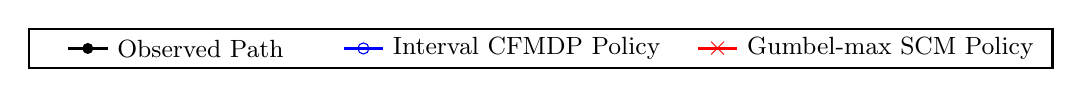
\begin{tikzpicture}[scale=1.0, every node/.style={scale=1.0}]
            \draw[thick, black] (-3, -0.25) rectangle (10, 0.25);
            %
            \draw[black, line width=1pt] (-2.5, 0.0) -- (-2,0.0);
            \fill[black] (-2.25,0.0) circle (2pt); %
            \node[right] at (-2,0.0) {\small Observed Path};
            
            %
            \draw[blue, line width=1pt] (1.0,0.0) -- (1.5,0.0);
            \node[draw=blue, circle, minimum size=4pt, inner sep=0pt] at (1.25,0.0) {}; %
            \node[right] at (1.5,0.0) {\small Interval CFMDP Policy};
            
            %
            \draw[red, line width=1pt] (5.5,0) -- (6,0);
            \node[red] at (5.75,0) {$\boldsymbol{\times}$}; %
            \node[right] at (6,0) {\small Gumbel-max SCM Policy};
        \end{tikzpicture}
    }\\
    %
    \subfigure[\footnotesize Lowest cumulative reward: Interval CFMDP ($312$), Gumbel-max SCM ($312$)]{%
        \resizebox{0.76\columnwidth}{!}{
             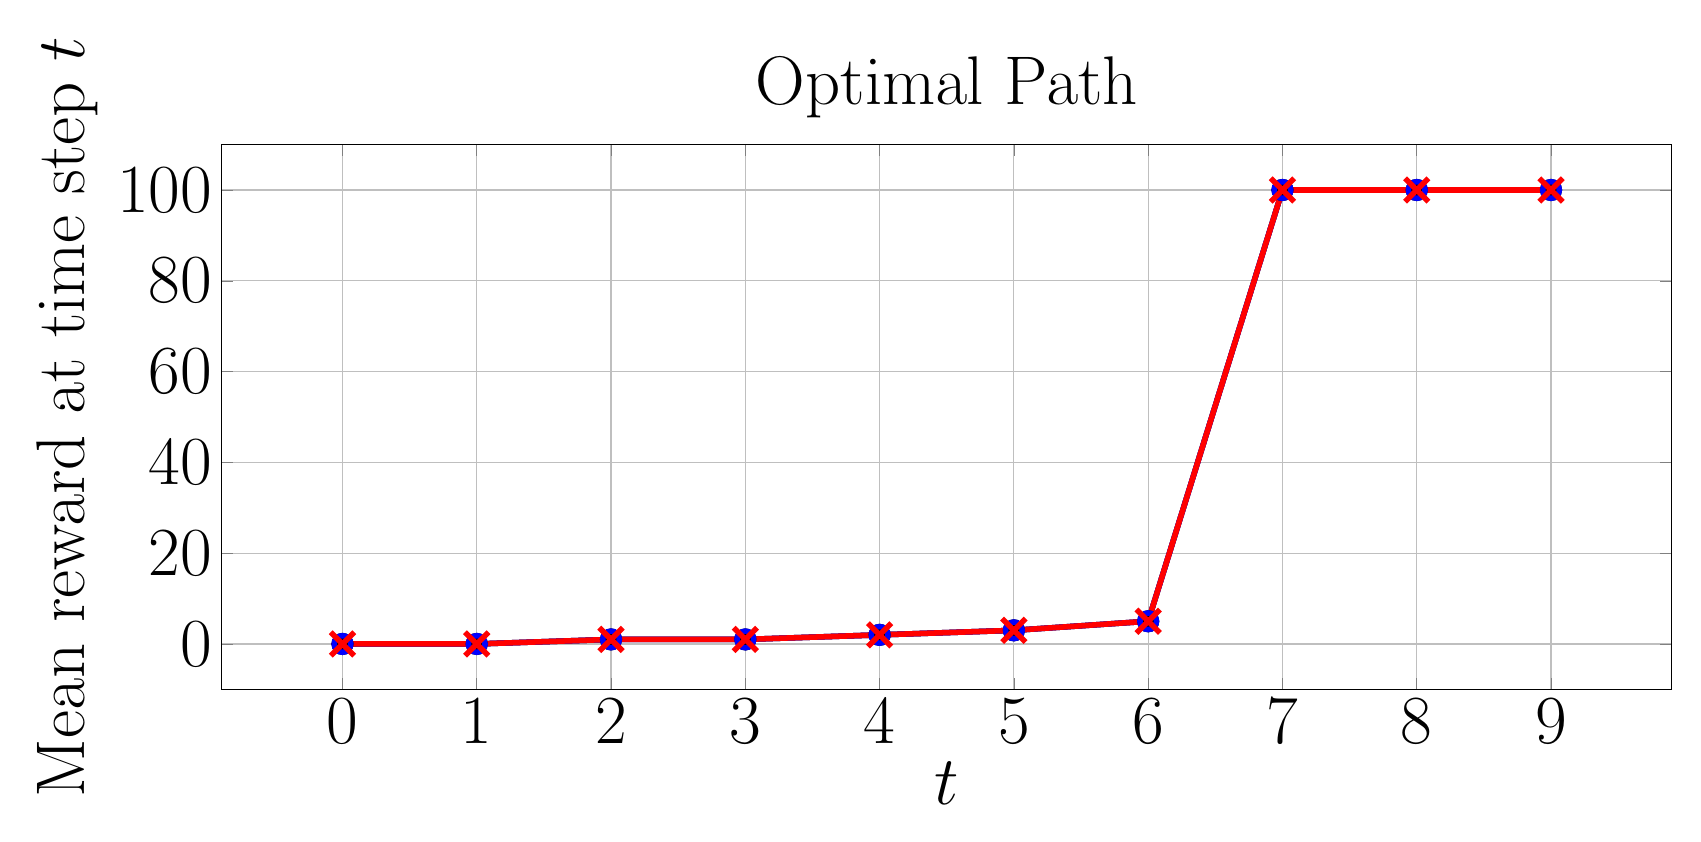
\begin{tikzpicture}
                \begin{axis}[
                    xlabel={$t$},
                    ylabel={Mean reward at time step $t$},
                    title={Optimal Path},
                    grid=both,
                    width=20cm, height=8.5cm,
                    every axis/.style={font=\Huge},
                    %
                ]
                \addplot[
                    color=black, %
                    mark=*, %
                    line width=2pt,
                    mark size=3pt,
                    error bars/.cd,
                    y dir=both, %
                    y explicit, %
                    error bar style={line width=1pt,solid},
                    error mark options={line width=1pt,mark size=4pt,rotate=90}
                ]
                coordinates {
                    (0, 0.0)  +- (0, 0.0)
                    (1, 0.0)  +- (0, 0.0) 
                    (2, 1.0)  +- (0, 0.0) 
                    (3, 1.0)  +- (0, 0.0)
                    (4, 2.0)  +- (0, 0.0)
                    (5, 3.0) +- (0, 0.0)
                    (6, 5.0) +- (0, 0.0)
                    (7, 100.0) +- (0, 0.0)
                    (8, 100.0) +- (0, 0.0)
                    (9, 100.0) +- (0, 0.0)
                };
                %
                \addplot[
                    color=blue, %
                    mark=o, %
                    line width=2pt,
                    mark size=3pt,
                    error bars/.cd,
                    y dir=both, %
                    y explicit, %
                    error bar style={line width=1pt,solid},
                    error mark options={line width=1pt,mark size=4pt,rotate=90}
                ]
                 coordinates {
                    (0, 0.0)  +- (0, 0.0)
                    (1, 0.0)  +- (0, 0.0) 
                    (2, 1.0)  +- (0, 0.0) 
                    (3, 1.0)  +- (0, 0.0)
                    (4, 2.0)  +- (0, 0.0)
                    (5, 3.0) +- (0, 0.0)
                    (6, 5.0) +- (0, 0.0)
                    (7, 100.0) +- (0, 0.0)
                    (8, 100.0) +- (0, 0.0)
                    (9, 100.0) +- (0, 0.0)
                };
                %
                \addplot[
                    color=red, %
                    mark=x, %
                    line width=2pt,
                    mark size=6pt,
                    error bars/.cd,
                    y dir=both, %
                    y explicit, %
                    error bar style={line width=1pt,solid},
                    error mark options={line width=1pt,mark size=4pt,rotate=90}
                ]
                coordinates {
                    (0, 0.0)  +- (0, 0.0)
                    (1, 0.0)  +- (0, 0.0) 
                    (2, 1.0)  +- (0, 0.0) 
                    (3, 1.0)  +- (0, 0.0)
                    (4, 2.0)  +- (0, 0.0)
                    (5, 3.0) +- (0, 0.0)
                    (6, 5.0) +- (0, 0.0)
                    (7, 100.0) +- (0, 0.0)
                    (8, 100.0) +- (0, 0.0)
                    (9, 100.0) +- (0, 0.0)
                };
                \end{axis}
            \end{tikzpicture}
         }
    }
    \hspace{1cm}
    \subfigure[\footnotesize Lowest cumulative reward: Interval CFMDP ($19$), Gumbel-max SCM ($-88$)]{%
         \resizebox{0.76\columnwidth}{!}{
            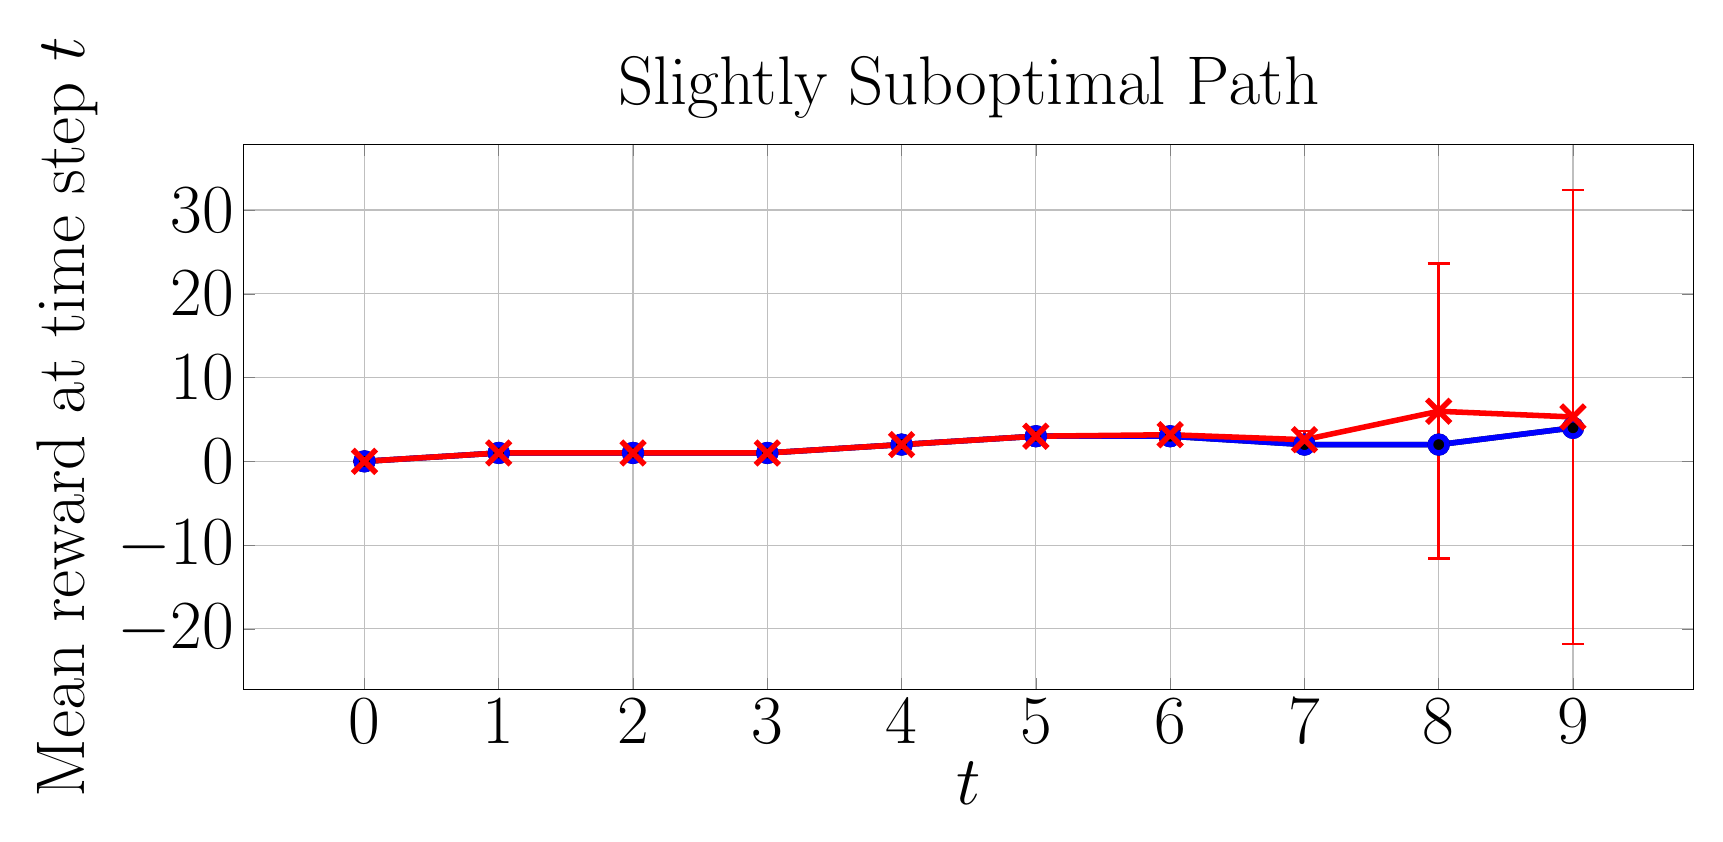
\begin{tikzpicture}
                \begin{axis}[
                    xlabel={$t$},
                    ylabel={Mean reward at time step $t$},
                    title={Slightly Suboptimal Path},
                    grid=both,
                    width=20cm, height=8.5cm,
                    every axis/.style={font=\Huge},
                    %
                ]
                \addplot[
                    color=black, %
                    mark=*, %
                    line width=2pt,
                    mark size=3pt,
                    error bars/.cd,
                    y dir=both, %
                    y explicit, %
                    error bar style={line width=1pt,solid},
                    error mark options={line width=1pt,mark size=4pt,rotate=90}
                ]
              coordinates {
                    (0, 0.0)  +- (0, 0.0)
                    (1, 1.0)  +- (0, 0.0) 
                    (2, 1.0)  +- (0, 0.0) 
                    (3, 1.0)  +- (0, 0.0)
                    (4, 2.0)  +- (0, 0.0)
                    (5, 3.0) +- (0, 0.0)
                    (6, 3.0) +- (0, 0.0)
                    (7, 2.0) +- (0, 0.0)
                    (8, 2.0) +- (0, 0.0)
                    (9, 4.0) +- (0, 0.0)
                };
                %
                \addplot[
                    color=blue, %
                    mark=o, %
                    line width=2pt,
                    mark size=3pt,
                    error bars/.cd,
                    y dir=both, %
                    y explicit, %
                    error bar style={line width=1pt,solid},
                    error mark options={line width=1pt,mark size=4pt,rotate=90}
                ]
              coordinates {
                    (0, 0.0)  +- (0, 0.0)
                    (1, 1.0)  +- (0, 0.0) 
                    (2, 1.0)  +- (0, 0.0) 
                    (3, 1.0)  +- (0, 0.0)
                    (4, 2.0)  +- (0, 0.0)
                    (5, 3.0) +- (0, 0.0)
                    (6, 3.0) +- (0, 0.0)
                    (7, 2.0) +- (0, 0.0)
                    (8, 2.0) +- (0, 0.0)
                    (9, 4.0) +- (0, 0.0)
                };
                %
                \addplot[
                    color=red, %
                    mark=x, %
                    line width=2pt,
                    mark size=6pt,
                    error bars/.cd,
                    y dir=both, %
                    y explicit, %
                    error bar style={line width=1pt,solid},
                    error mark options={line width=1pt,mark size=4pt,rotate=90}
                ]
                coordinates {
                    (0, 0.0)  +- (0, 0.0)
                    (1, 1.0)  +- (0, 0.0) 
                    (2, 1.0)  +- (0, 0.0) 
                    (3, 1.0)  +- (0, 0.0)
                    (4, 2.0)  += (0, 0.0)
                    (5, 3.0)  += (0, 0.0)
                    (6, 3.17847) += (0, 0.62606746) -= (0, 0.62606746)
                    (7, 2.5832885) += (0, 1.04598233) -= (0, 1.04598233)
                    (8, 5.978909) += (0, 17.60137623) -= (0, 17.60137623)
                    (9, 5.297059) += (0, 27.09227512) -= (0, 27.09227512)
                };
                \end{axis}
            \end{tikzpicture}
         }
    }\\[-1.5pt]
    \subfigure[\footnotesize Lowest cumulative reward: Interval CFMDP ($14$), Gumbel-max SCM ($-598$)]{%
         \resizebox{0.76\columnwidth}{!}{
             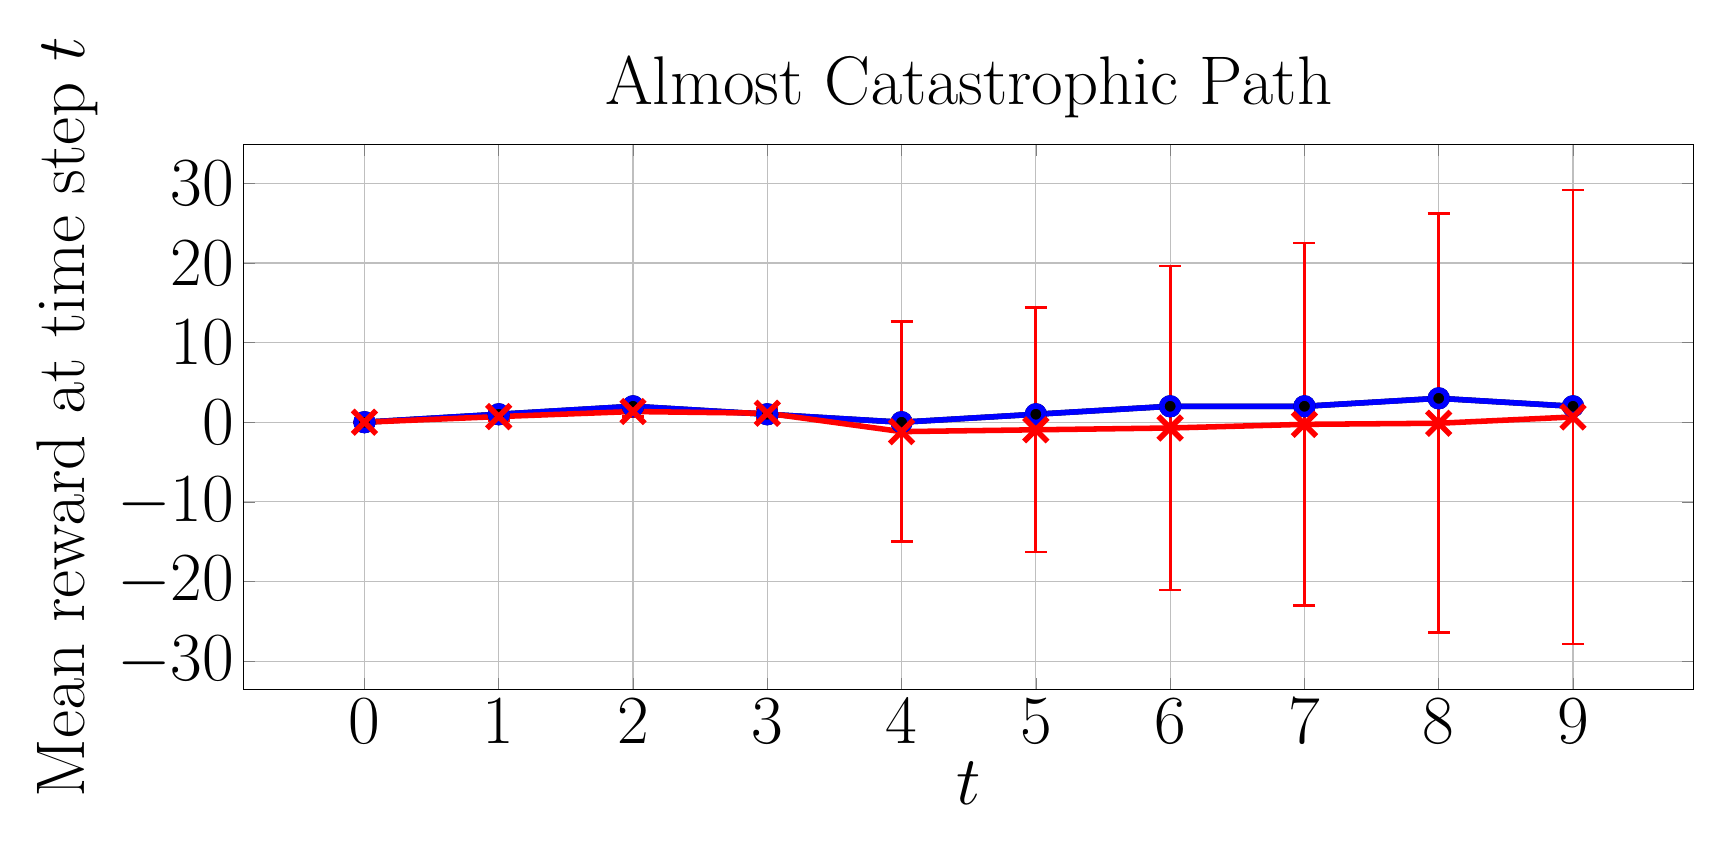
\begin{tikzpicture}
                \begin{axis}[
                    xlabel={$t$},
                    ylabel={Mean reward at time step $t$},
                    title={Almost Catastrophic Path},
                    grid=both,
                    width=20cm, height=8.5cm,
                    every axis/.style={font=\Huge},
                    %
                ]
                \addplot[
                    color=black, %
                    mark=*, %
                    line width=2pt,
                    mark size=3pt,
                    error bars/.cd,
                    y dir=both, %
                    y explicit, %
                    error bar style={line width=1pt,solid},
                    error mark options={line width=1pt,mark size=4pt,rotate=90}
                ]
                coordinates {
                    (0, 0.0)  +- (0, 0.0)
                    (1, 1.0)  +- (0, 0.0) 
                    (2, 2.0)  +- (0, 0.0) 
                    (3, 1.0)  +- (0, 0.0)
                    (4, 0.0)  +- (0, 0.0)
                    (5, 1.0) +- (0, 0.0)
                    (6, 2.0) +- (0, 0.0)
                    (7, 2.0) +- (0, 0.0)
                    (8, 3.0) +- (0, 0.0)
                    (9, 2.0) +- (0, 0.0)
                };
                %
                \addplot[
                    color=blue, %
                    mark=o, %
                    line width=2pt,
                    mark size=3pt,
                    error bars/.cd,
                    y dir=both, %
                    y explicit, %
                    error bar style={line width=1pt,solid},
                    error mark options={line width=1pt,mark size=4pt,rotate=90}
                ]
                coordinates {
                    (0, 0.0)  +- (0, 0.0)
                    (1, 1.0)  +- (0, 0.0) 
                    (2, 2.0)  +- (0, 0.0) 
                    (3, 1.0)  +- (0, 0.0)
                    (4, 0.0)  +- (0, 0.0)
                    (5, 1.0) +- (0, 0.0)
                    (6, 2.0) +- (0, 0.0)
                    (7, 2.0) +- (0, 0.0)
                    (8, 3.0) +- (0, 0.0)
                    (9, 2.0) +- (0, 0.0)
                };
                %
                \addplot[
                    color=red, %
                    mark=x, %
                    line width=2pt,
                    mark size=6pt,
                    error bars/.cd,
                    y dir=both, %
                    y explicit, %
                    error bar style={line width=1pt,solid},
                    error mark options={line width=1pt,mark size=4pt,rotate=90}
                ]
                coordinates {
                    (0, 0.0)  +- (0, 0.0)
                    (1, 0.7065655)  +- (0, 0.4553358) 
                    (2, 1.341673)  +- (0, 0.67091621) 
                    (3, 1.122926)  +- (0, 0.61281824)
                    (4, -1.1821935)  +- (0, 13.82444042)
                    (5, -0.952399)  +- (0, 15.35195457)
                    (6, -0.72672) +- (0, 20.33508414)
                    (7, -0.268983) +- (0, 22.77861454)
                    (8, -0.1310835) +- (0, 26.31013314)
                    (9, 0.65806) +- (0, 28.50670214)
                };
                %
            %
            %
            %
            %
            %
            %
            %
            %
            %
            %
            %
            %
            %
            %
            %
            %
            %
            %
                \end{axis}
            \end{tikzpicture}
         }
    }
    \hspace{1cm}
    \subfigure[\footnotesize Lowest cumulative reward: Interval CFMDP ($-698$), Gumbel-max SCM ($-698$)]{%
         \resizebox{0.76\columnwidth}{!}{
            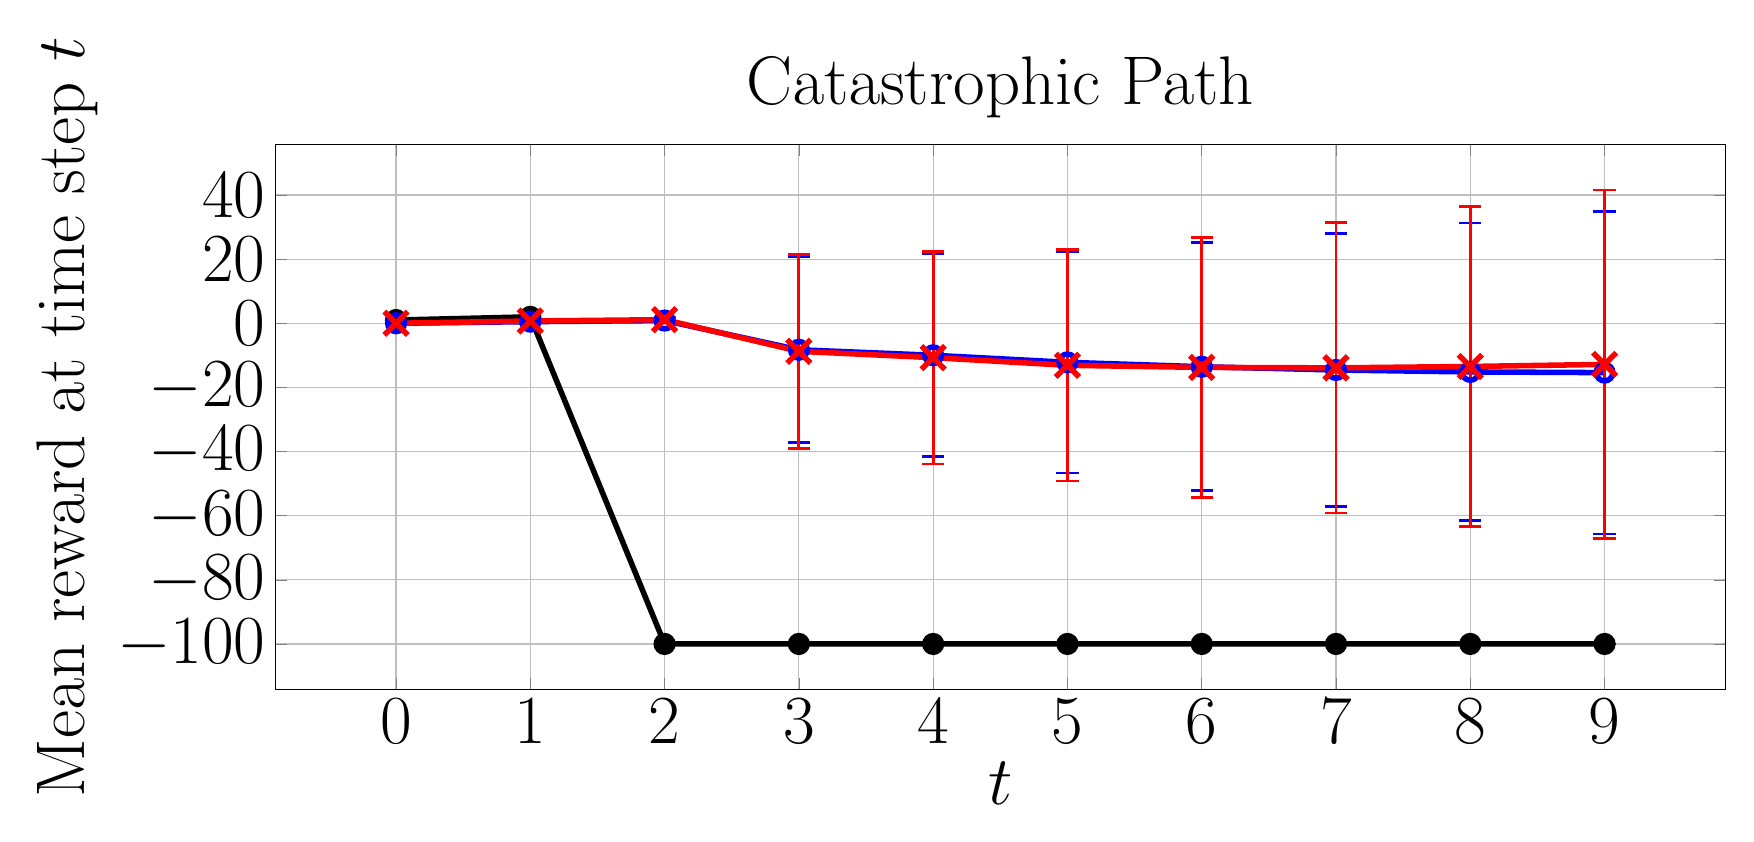
\begin{tikzpicture}
                \begin{axis}[
                    xlabel={$t$},
                    ylabel={Mean reward at time step $t$},
                    title={Catastrophic Path},
                    grid=both,
                    width=20cm, height=8.5cm,
                    every axis/.style={font=\Huge},
                    %
                ]
                \addplot[
                    color=black, %
                    mark=*, %
                    line width=2pt,
                    mark size=3pt,
                    error bars/.cd,
                    y dir=both, %
                    y explicit, %
                    error bar style={line width=1pt,solid},
                    error mark options={line width=1pt,mark size=4pt,rotate=90}
                ]
                coordinates {
                    (0, 1.0)  +- (0, 0.0)
                    (1, 2.0)  +- (0, 0.0) 
                    (2, -100.0)  +- (0, 0.0) 
                    (3, -100.0)  +- (0, 0.0)
                    (4, -100.0)  +- (0, 0.0)
                    (5, -100.0) +- (0, 0.0)
                    (6, -100.0) +- (0, 0.0)
                    (7, -100.0) +- (0, 0.0)
                    (8, -100.0) +- (0, 0.0)
                    (9, -100.0) +- (0, 0.0)
                };
                %
                \addplot[
                    color=blue, %
                    mark=o, %
                    line width=2pt,
                    mark size=3pt,
                    error bars/.cd,
                    y dir=both, %
                    y explicit, %
                    error bar style={line width=1pt,solid},
                    error mark options={line width=1pt,mark size=4pt,rotate=90}
                ]
                coordinates {
                    (0, 0.0)  +- (0, 0.0)
                    (1, 0.504814)  +- (0, 0.49997682) 
                    (2, 0.8439835)  +- (0, 0.76831917) 
                    (3, -8.2709165)  +- (0, 28.93656754)
                    (4, -9.981082)  +- (0, 31.66825363)
                    (5, -12.1776325) +- (0, 34.53463233)
                    (6, -13.556076) +- (0, 38.62845372)
                    (7, -14.574418) +- (0, 42.49603359)
                    (8, -15.1757075) +- (0, 46.41913968)
                    (9, -15.3900395) +- (0, 50.33563368)
                };
                %
                \addplot[
                    color=red, %
                    mark=x, %
                    line width=2pt,
                    mark size=6pt,
                    error bars/.cd,
                    y dir=both, %
                    y explicit, %
                    error bar style={line width=1pt,solid},
                    error mark options={line width=1pt,mark size=4pt,rotate=90}
                ]
                coordinates {
                    (0, 0.0)  +- (0, 0.0)
                    (1, 0.701873)  +- (0, 0.45743556) 
                    (2, 1.1227805)  +- (0, 0.73433129) 
                    (3, -8.7503255)  +- (0, 30.30257976)
                    (4, -10.722092)  +- (0, 33.17618589)
                    (5, -13.10721)  +- (0, 36.0648089)
                    (6, -13.7631645) +- (0, 40.56553451)
                    (7, -13.909043) +- (0, 45.23829402)
                    (8, -13.472517) +- (0, 49.96270296)
                    (9, -12.8278835) +- (0, 54.38618735)
                };
                %
            %
            %
            %
            %
            %
            %
            %
            %
            %
            %
            %
            %
            %
            %
            %
            %
            %
            %
                \end{axis}
            \end{tikzpicture}
         }
    }
    \caption{Average instant reward of CF paths induced by policies on GridWorld $p=0.4$.}
    \label{fig: reward p=0.4}
\end{figure*}

\subsection{Experimental Setup}
To compare policy performance, we measure the average rewards of counterfactual paths induced by our policy and the Gumbel-max policy by uniformly sampling $200$ counterfactual MDPs from the ICFMDP and generating $10,000$ counterfactual paths over each sampled CFMDP. \jl{Since the interval CFMDP depends on the observed path, we select $4$  paths of varying optimality to evaluate how the observed path impacts the performance of both policies: an optimal path, a slightly suboptimal path that could reach the optimal reward with a few changes, a catastrophic path that enters a catastrophic, terminal state with low reward, and an almost catastrophic path that was close to entering a catastrophic state.} When measuring the average probability bound widths and execution time needed to generate the ICFMDPs, we averaged over $20$ randomly generated observed paths
\footnote{Further training details are provided in Appendix \ref{app: training details}, and the code is provided at \href{https://github.com/ddv-lab/robust-cf-inference-in-MDPs}{https://github.com/ddv-lab/robust-cf-inference-in-MDPs}
%
%
.}.

\subsection{GridWorld}
\jl{The GridWorld MDP is a $4 \times 4$ grid where an agent must navigate from the top-left corner to the goal state in the bottom-right corner, avoiding a dangerous terminal state in the centre. At each time step, the agent can move up, down, left, or right, but there is a small probability (controlled by hyper-parameter $p$) of moving in an unintended direction. As the agent nears the goal, the reward for each state increases, culminating in a reward of $+100$ for reaching the goal. Entering the dangerous state results in a penalty of $-100$. We use two versions of GridWorld: a less stochastic version with $p=0.9$ (i.e., $90$\% chance of moving in the chosen direction) and a more stochastic version with $p=0.4$.}

\paragraph{GridWorld ($p=0.9$)}
When $p=0.9$, the counterfactual probability bounds are typically narrow (see Table \ref{tab:nonzero_probs} for average measurements). Consequently, as shown in Figure \ref{fig: reward p=0.9}, both policies are nearly identical and perform similarly well across the optimal, slightly suboptimal, and catastrophic paths.
%
However, for the almost catastrophic path, the interval CFMDP path is more conservative and follows the observed path more closely (as this is where the probability bounds are narrowest), which typically requires one additional step to reach the goal state than the Gumbel-max SCM policy.
%

\paragraph{GridWorld ($p=0.4$)}
\jl{When $p=0.4$, the GridWorld environment becomes more uncertain, increasing the risk of entering the dangerous state even if correct actions are chosen. Thus, as shown in Figure \ref{fig: reward p=0.4}, the interval CFMDP policy adopts a more conservative approach, avoiding deviation from the observed policy if it cannot guarantee higher counterfactual rewards (see the slightly suboptimal and almost catastrophic paths), whereas the Gumbel-max SCM is inconsistent: it can yield higher rewards, but also much lower rewards, reflected in the wide error bars.} For the catastrophic path, both policies must deviate from the observed path to achieve a higher reward and, in this case, perform similarly.
%
%
%
%
\subsection{Sepsis}
The Sepsis MDP \citep{oberst2019counterfactual} simulates trajectories of Sepsis patients. Each state consists of four vital signs (heart rate, blood pressure, oxygen concentration, and glucose levels), categorised as low, normal, or high.
and three treatments that can be toggled on/off at each time step (8 actions in total). Unlike \citet{oberst2019counterfactual}, we scale rewards based on the number of out-of-range vital signs, between $-1000$ (patient dies) and $1000$ (patient discharged). \jl{Like the GridWorld $p=0.4$ experiment, the Sepsis MDP is highly uncertain, as many states are equally likely to lead to optimal and poor outcomes. Thus, as shown in Figure \ref{fig: reward sepsis}, both policies follow the observed optimal and almost catastrophic paths to guarantee rewards are no worse than the observation.} However, improving the catastrophic path requires deviating from the observation. Here, the Gumbel-max SCM policy, on average, performs better than the interval CFMDP policy. But, since both policies have lower bounds clipped at $-1000$, neither policy reliably improves over the observation. In contrast, for the slightly suboptimal path, the interval CFMDP policy performs significantly better, shown by its higher lower bounds. 
Moreover, in these two cases, the worst-case counterfactual path generated by the interval CFMDP policy is better than that of the Gumbel-max SCM policy,
indicating its greater robustness.
%
\begin{figure*}
    \centering
     \resizebox{0.6\textwidth}{!}{
        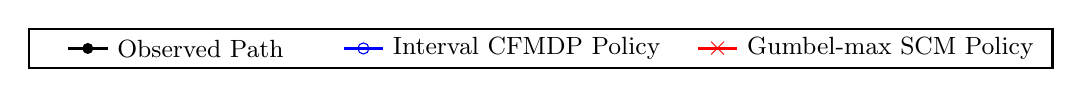
\begin{tikzpicture}[scale=1.0, every node/.style={scale=1.0}]
            \draw[thick, black] (-3, -0.25) rectangle (10, 0.25);
            %
            \draw[black, line width=1pt] (-2.5, 0.0) -- (-2,0.0);
            \fill[black] (-2.25,0.0) circle (2pt); %
            \node[right] at (-2,0.0) {\small Observed Path};
            
            %
            \draw[blue, line width=1pt] (1.0,0.0) -- (1.5,0.0);
            \node[draw=blue, circle, minimum size=4pt, inner sep=0pt] at (1.25,0.0) {}; %
            \node[right] at (1.5,0.0) {\small Interval CFMDP Policy};
            
            %
            \draw[red, line width=1pt] (5.5,0) -- (6,0);
            \node[red] at (5.75,0) {$\boldsymbol{\times}$}; %
            \node[right] at (6,0) {\small Gumbel-max SCM Policy};
        \end{tikzpicture}
    }\\
    \subfigure[\footnotesize Lowest cumulative reward: Interval CFMDP ($8000$), Gumbel-max SCM ($8000$)]{%
         \resizebox{0.76\columnwidth}{!}{
             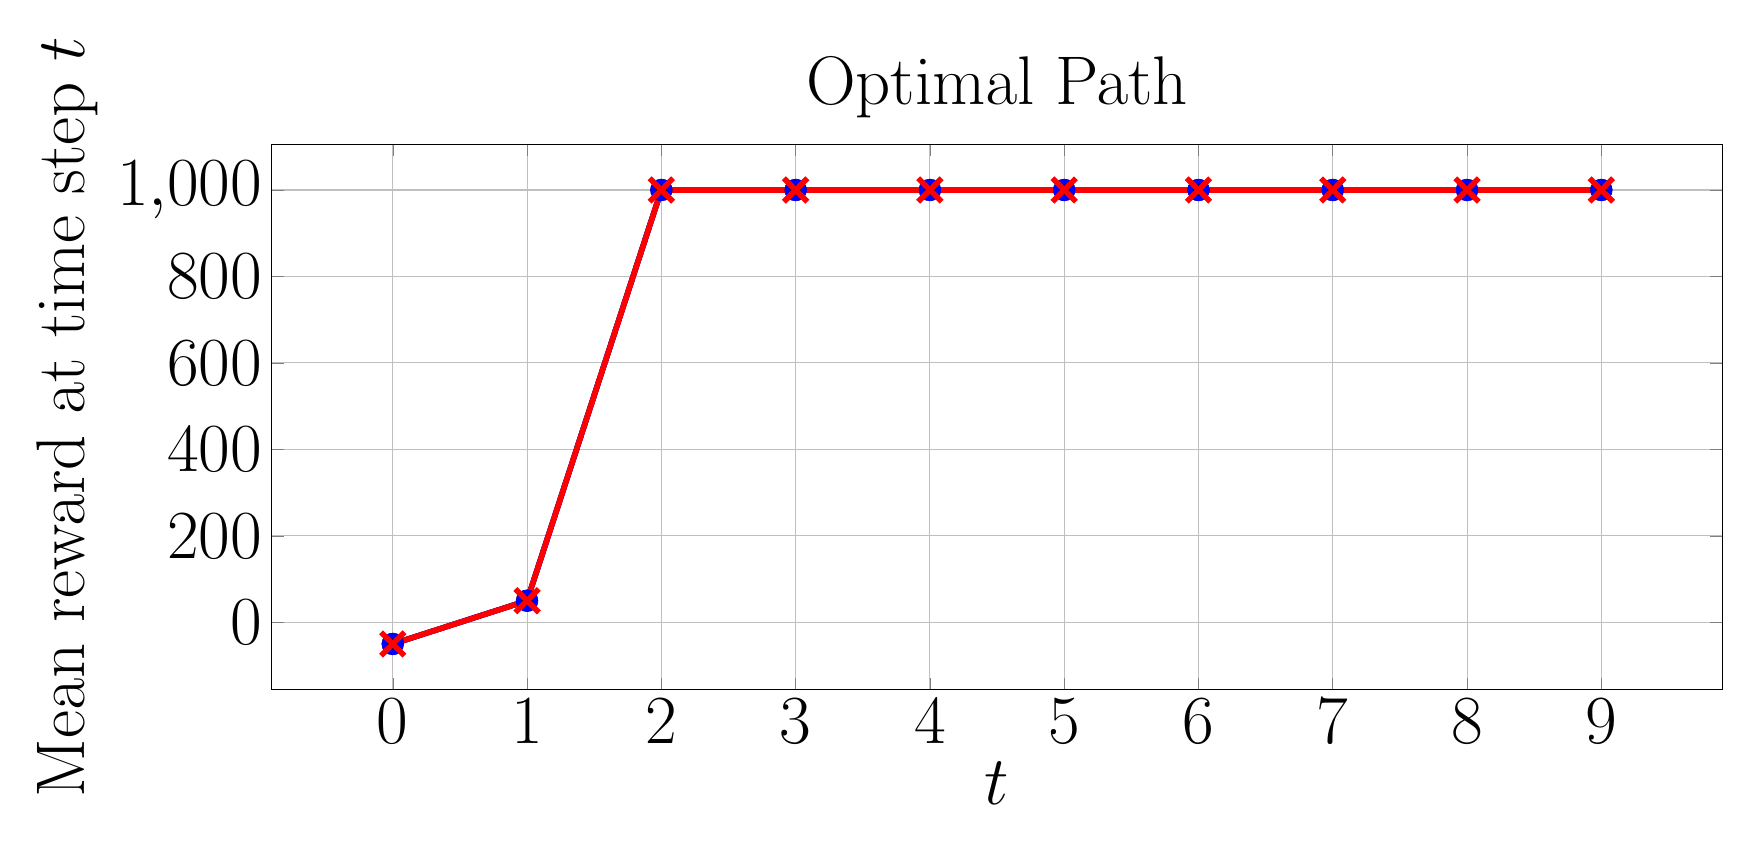
\begin{tikzpicture}
                \begin{axis}[
                    xlabel={$t$},
                    ylabel={Mean reward at time step $t$},
                    title={Optimal Path},
                    grid=both,
                    width=20cm, height=8.5cm,
                    every axis/.style={font=\Huge},
                    %
                ]
                \addplot[
                    color=black, %
                    mark=*, %
                    line width=2pt,
                    mark size=3pt,
                ]
                coordinates {
                    (0, -50.0)
                    (1, 50.0)
                    (2, 1000.0)
                    (3, 1000.0)
                    (4, 1000.0)
                    (5, 1000.0)
                    (6, 1000.0)
                    (7, 1000.0)
                    (8, 1000.0)
                    (9, 1000.0)
                };
                %
                \addplot[
                    color=blue, %
                    mark=o, %
                    line width=2pt,
                    mark size=3pt,
                    error bars/.cd,
                    y dir=both, %
                    y explicit, %
                    error bar style={line width=1pt,solid},
                    error mark options={line width=1pt,mark size=4pt,rotate=90}
                ]
                coordinates {
                    (0, -50.0)  +- (0, 0.0)
                    (1, 50.0)  +- (0, 0.0) 
                    (2, 1000.0)  +- (0, 0.0) 
                    (3, 1000.0)  +- (0, 0.0)
                    (4, 1000.0)  +- (0, 0.0)
                    (5, 1000.0) +- (0, 0.0)
                    (6, 1000.0) +- (0, 0.0)
                    (7, 1000.0) +- (0, 0.0)
                    (8, 1000.0) +- (0, 0.0)
                    (9, 1000.0) +- (0, 0.0)
                };
                %
                \addplot[
                    color=red, %
                    mark=x, %
                    line width=2pt,
                    mark size=6pt,
                    error bars/.cd,
                    y dir=both, %
                    y explicit, %
                    error bar style={line width=1pt,solid},
                    error mark options={line width=1pt,mark size=4pt,rotate=90}
                ]
                coordinates {
                    (0, -50.0)  +- (0, 0.0)
                    (1, 50.0)  +- (0, 0.0) 
                    (2, 1000.0)  +- (0, 0.0) 
                    (3, 1000.0)  +- (0, 0.0)
                    (4, 1000.0)  +- (0, 0.0)
                    (5, 1000.0) +- (0, 0.0)
                    (6, 1000.0) +- (0, 0.0)
                    (7, 1000.0) +- (0, 0.0)
                    (8, 1000.0) +- (0, 0.0)
                    (9, 1000.0) +- (0, 0.0)
                };
                %
                \end{axis}
            \end{tikzpicture}
         }
    }
    \hspace{1cm}
    \subfigure[\footnotesize Lowest cumulative reward: Interval CFMDP ($-5980$), Gumbel-max SCM ($-8000$)]{%
         \resizebox{0.76\columnwidth}{!}{
            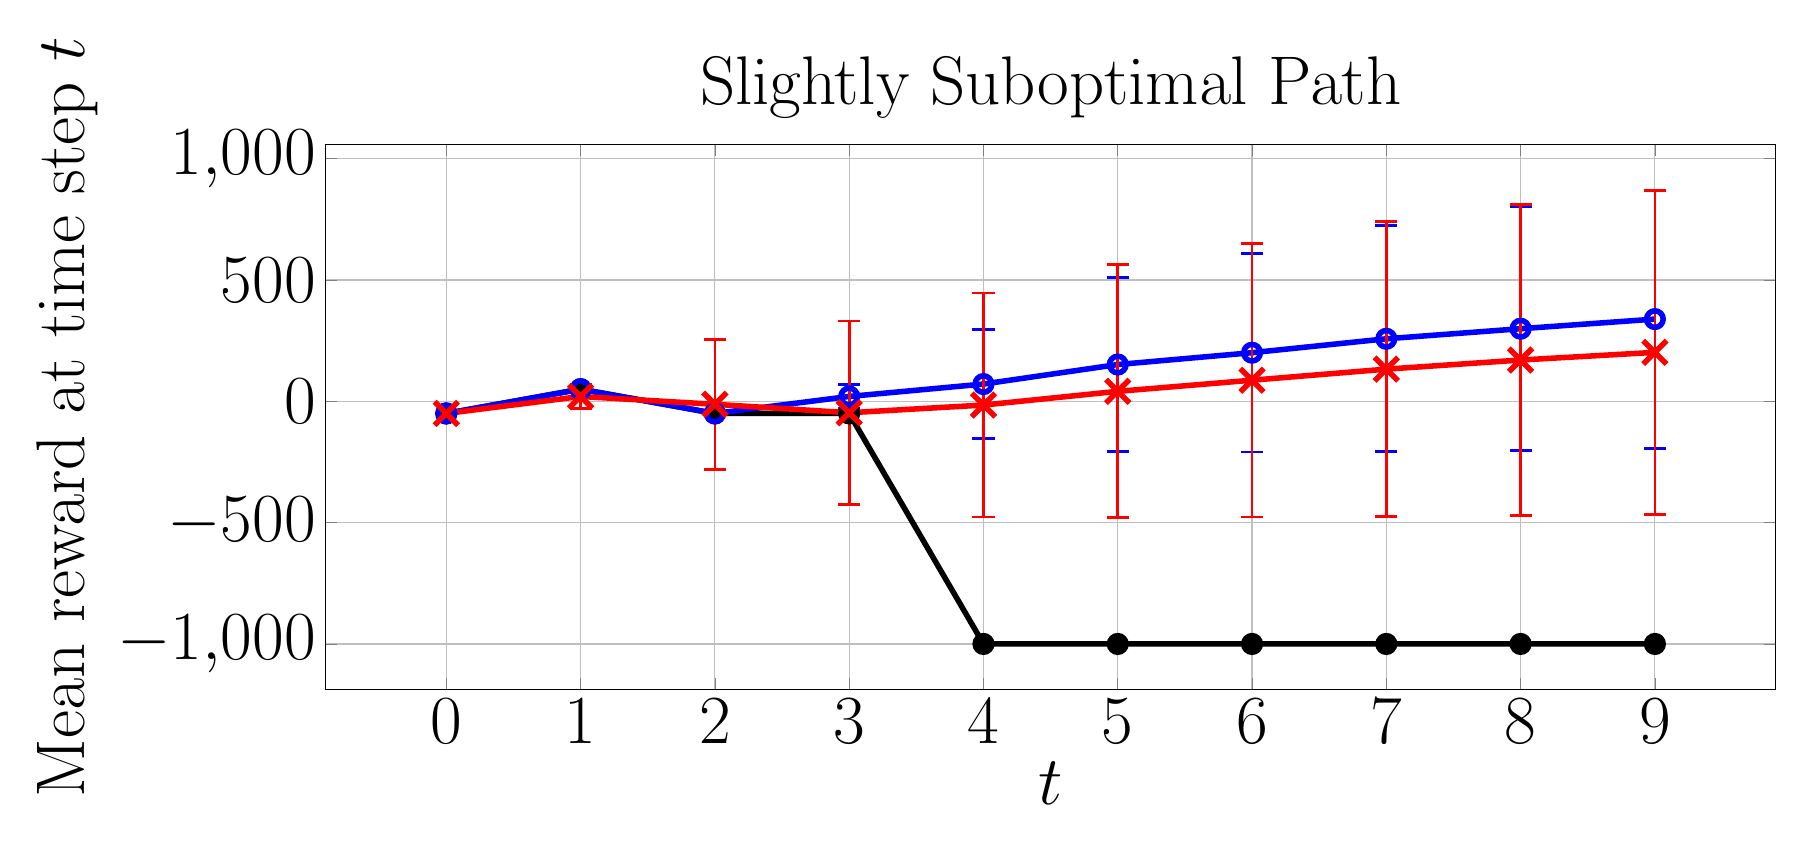
\begin{tikzpicture}
                \begin{axis}[
                    xlabel={$t$},
                    ylabel={Mean reward at time step $t$},
                    title={Slightly Suboptimal Path},
                    grid=both,
                    width=20cm, height=8.5cm,
                    every axis/.style={font=\Huge},
                    %
                ]
               \addplot[
                    color=black, %
                    mark=*, %
                    line width=2pt,
                    mark size=3pt,
                ]
                coordinates {
                    (0, -50.0)
                    (1, 50.0)
                    (2, -50.0)
                    (3, -50.0)
                    (4, -1000.0)
                    (5, -1000.0)
                    (6, -1000.0)
                    (7, -1000.0)
                    (8, -1000.0)
                    (9, -1000.0)
                };
                %
                \addplot[
                    color=blue, %
                    mark=o, %
                    line width=2pt,
                    mark size=3pt,
                    error bars/.cd,
                    y dir=both, %
                    y explicit, %
                    error bar style={line width=1pt,solid},
                    error mark options={line width=1pt,mark size=4pt,rotate=90}
                ]
                coordinates {
                    (0, -50.0)  +- (0, 0.0)
                    (1, 50.0)  +- (0, 0.0) 
                    (2, -50.0)  +- (0, 0.0) 
                    (3, 20.0631)  +- (0, 49.97539413)
                    (4, 71.206585)  +- (0, 226.02033693)
                    (5, 151.60797) +- (0, 359.23292559)
                    (6, 200.40593) +- (0, 408.86185176)
                    (7, 257.77948) +- (0, 466.10372804)
                    (8, 299.237465) +- (0, 501.82579506)
                    (9, 338.9129) +- (0, 532.06124996)
                };
                %
                \addplot[
                    color=red, %
                    mark=x, %
                    line width=2pt,
                    mark size=6pt,
                    error bars/.cd,
                    y dir=both, %
                    y explicit, %
                    error bar style={line width=1pt,solid},
                    error mark options={line width=1pt,mark size=4pt,rotate=90}
                ]
                coordinates {
                    (0, -50.0)  +- (0, 0.0)
                    (1, 20.00736)  +- (0, 49.99786741) 
                    (2, -12.282865)  +- (0, 267.598755) 
                    (3, -47.125995)  +- (0, 378.41755832)
                    (4, -15.381965)  +- (0, 461.77616558)
                    (5, 41.15459) +- (0, 521.53189262)
                    (6, 87.01595) +- (0, 564.22243126 )
                    (7, 132.62376) +- (0, 607.31338037)
                    (8, 170.168145) +- (0, 641.48013693)
                    (9, 201.813135) +- (0, 667.29441777)
                };
                %
                %
                %
                %
                %
                %
                %
                %
                %
                %
                %
                %
                %
                %
                %
                %
                %
                %
                %
                \end{axis}
            \end{tikzpicture}
         }
    }\\[-1.5pt]
    \subfigure[\footnotesize Lowest cumulative reward: Interval CFMDP ($100$), Gumbel-max SCM ($100$)]{%
         \resizebox{0.76\columnwidth}{!}{
             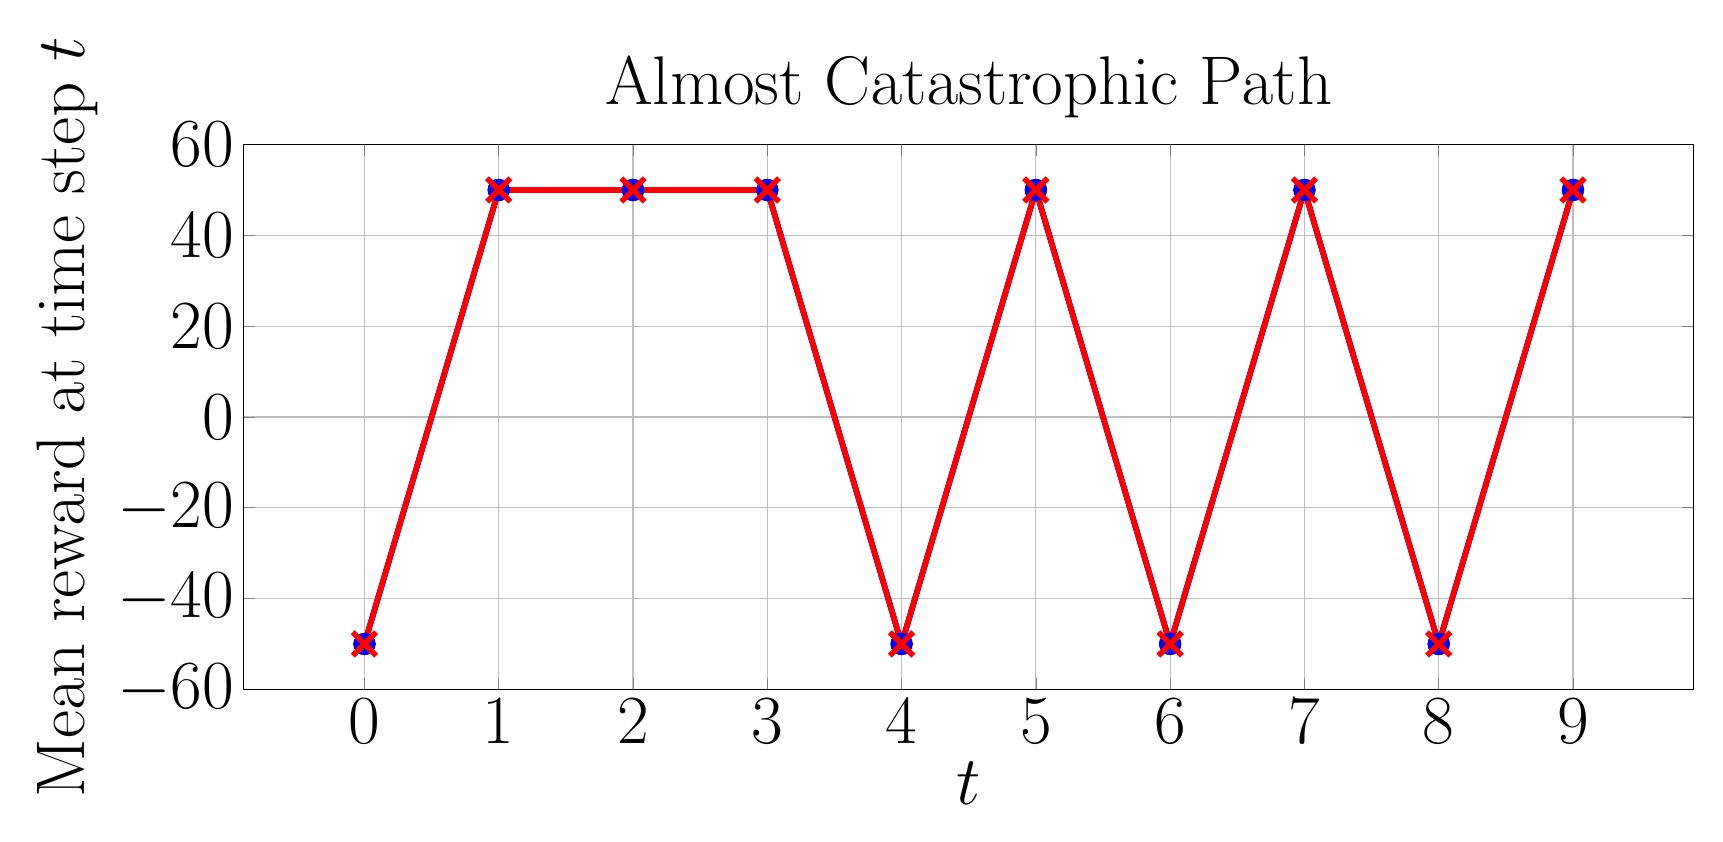
\begin{tikzpicture}
                \begin{axis}[
                    xlabel={$t$},
                    ylabel={Mean reward at time step $t$},
                    title={Almost Catastrophic Path},
                    grid=both,
                    every axis/.style={font=\Huge},
                    width=20cm, height=8.5cm,
                    %
                ]
               \addplot[
                    color=black, %
                    mark=*, %
                    line width=2pt,
                    mark size=3pt,
                ]
                coordinates {
                    (0, -50.0)
                    (1, 50.0)
                    (2, 50.0)
                    (3, 50.0)
                    (4, -50.0)
                    (5, 50.0)
                    (6, -50.0)
                    (7, 50.0)
                    (8, -50.0)
                    (9, 50.0)
                };
                %
                %
                \addplot[
                    color=blue, %
                    mark=o, %
                    line width=2pt,
                    mark size=3pt,
                    error bars/.cd,
                    y dir=both, %
                    y explicit, %
                    error bar style={line width=1pt,solid},
                    error mark options={line width=1pt,mark size=4pt,rotate=90}
                ]
                coordinates {
                    (0, -50.0)  +- (0, 0.0)
                    (1, 50.0)  +- (0, 0.0) 
                    (2, 50.0)  +- (0, 0.0) 
                    (3, 50.0)  +- (0, 0.0)
                    (4, -50.0)  +- (0, 0.0)
                    (5, 50.0) +- (0, 0.0)
                    (6, -50.0) +- (0, 0.0)
                    (7, 50.0) +- (0, 0.0)
                    (8, -50.0) +- (0, 0.0)
                    (9, 50.0) +- (0, 0.0)
                };
                %
                \addplot[
                    color=red, %
                    mark=x, %
                    line width=2pt,
                    mark size=6pt,
                    error bars/.cd,
                    y dir=both, %
                    y explicit, %
                    error bar style={line width=1pt,solid},
                    error mark options={line width=1pt,mark size=4pt,rotate=90}
                ]
                coordinates {
                    (0, -50.0)  +- (0, 0.0)
                    (1, 50.0)  +- (0, 0.0) 
                    (2, 50.0)  +- (0, 0.0) 
                    (3, 50.0)  +- (0, 0.0)
                    (4, -50.0)  +- (0, 0.0)
                    (5, 50.0) +- (0, 0.0)
                    (6, -50.0) +- (0, 0.0)
                    (7, 50.0) +- (0, 0.0)
                    (8, -50.0) +- (0, 0.0)
                    (9, 50.0) +- (0, 0.0)
                };
                %
                %
                %
                %
                %
                %
                %
                %
                %
                %
                %
                %
                %
                %
                %
                %
                %
                %
                %
                \end{axis}
            \end{tikzpicture}
         }
    }
    \hspace{1cm}
    \subfigure[\footnotesize Lowest cumulative reward: Interval CFMDP ($-7150$), Gumbel-max SCM ($-9050$)]{%
         \resizebox{0.76\columnwidth}{!}{
            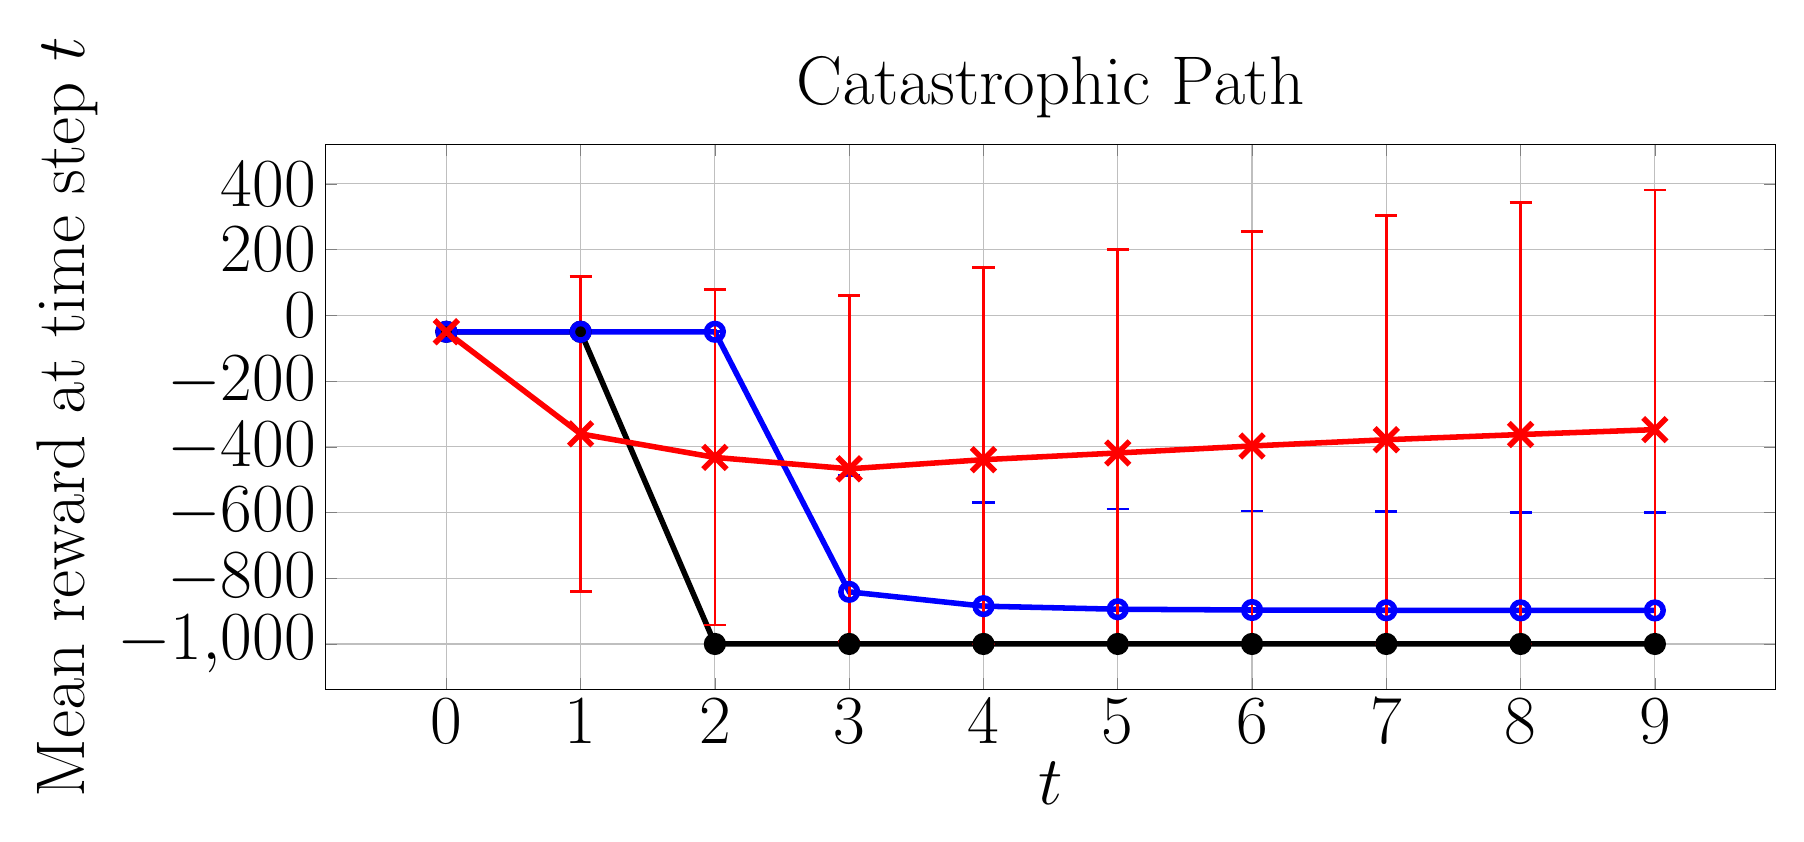
\begin{tikzpicture}
                \begin{axis}[
                    xlabel={$t$},
                    ylabel={Mean reward at time step $t$},
                    title={Catastrophic Path},
                    grid=both,
                    width=20cm, height=8.5cm,
                    every axis/.style={font=\Huge},
                    %
                ]
               \addplot[
                    color=black, %
                    mark=*, %
                    line width=2pt,
                    mark size=3pt,
                ]
                coordinates {
                    (0, -50.0)
                    (1, -50.0)
                    (2, -1000.0)
                    (3, -1000.0)
                    (4, -1000.0)
                    (5, -1000.0)
                    (6, -1000.0)
                    (7, -1000.0)
                    (8, -1000.0)
                    (9, -1000.0)
                };
                %
                %
                \addplot[
                    color=blue, %
                    mark=o, %
                    line width=2pt,
                    mark size=3pt,
                    error bars/.cd,
                    y dir=both, %
                    y explicit, %
                    error bar style={line width=1pt,solid},
                    error mark options={line width=1pt,mark size=4pt,rotate=90}
                ]
                coordinates {
                    (0, -50.0)  +- (0, 0.0)
                    (1, -50.0)  +- (0, 0.0) 
                    (2, -50.0)  +- (0, 0.0) 
                    (3, -841.440725)  += (0, 354.24605512) -= (0, 158.559275)
                    (4, -884.98225)  += (0, 315.37519669) -= (0, 115.01775)
                    (5, -894.330425) += (0, 304.88572805) -= (0, 105.669575)
                    (6, -896.696175) += (0, 301.19954514) -= (0, 103.303825)
                    (7, -897.4635) += (0, 299.61791279) -= (0, 102.5365)
                    (8, -897.77595) += (0, 298.80392585) -= (0, 102.22405)
                    (9, -897.942975) += (0, 298.32920557) -= (0, 102.057025)
                };
                %
                \addplot[
                    color=red, %
                    mark=x, %
                    line width=2pt,
                    mark size=6pt,
                    error bars/.cd,
                    y dir=both, %
                    y explicit, %
                    error bar style={line width=1pt,solid},
                    error mark options={line width=1pt,mark size=4pt,rotate=90}
                ]
            coordinates {
                    (0, -50.0)  +- (0, 0.0)
                    (1, -360.675265)  +- (0, 479.39812699) 
                    (2, -432.27629)  +- (0, 510.38620897) 
                    (3, -467.029545)  += (0, 526.36009628) -= (0, 526.36009628)
                    (4, -439.17429)  += (0, 583.96638919) -= (0, 560.82571)
                    (5, -418.82704) += (0, 618.43027478) -= (0, 581.17296)
                    (6, -397.464895) += (0, 652.67322574) -= (0, 602.535105)
                    (7, -378.49052) += (0, 682.85407033) -= (0, 621.50948)
                    (8, -362.654195) += (0, 707.01412023) -= (0, 637.345805)
                    (9, -347.737935) += (0, 729.29076479) -= (0, 652.262065)
                };
                %
                %
                %
                %
                %
                %
                %
                %
                %
                %
                %
                %
                %
                %
                %
                %
                %
                %
                %
                \end{axis}
            \end{tikzpicture}
         }
    }
    \caption{Average instant reward of CF paths induced by policies on Sepsis.}
    \label{fig: reward sepsis}
\end{figure*}

%
%
%
\subsection{Interval CFMDP Bounds}
%
%
Table \ref{tab:nonzero_probs} presents the mean counterfactual probability bound widths (excluding transitions where the upper bound is $0$) for each MDP, averaged over 20 observed paths. We compare the bounds under counterfactual stability (CS) and monotonicity (M) assumptions, CS alone, and no assumptions. This shows that the assumptions marginally reduce the bound widths, indicating the assumptions tighten the bounds without excluding too many causal models, as intended.
\renewcommand{\arraystretch}{1}

\begin{table}
\centering
\caption{Mean width of counterfactual probability bounds}
\resizebox{0.8\columnwidth}{!}{%
\begin{tabular}{|c|c|c|c|}
\hline
\multirow{2}{*}{\textbf{Environment}} & \multicolumn{3}{c|}{\textbf{Assumptions}} \\ \cline{2-4}
 & \textbf{CS + M} & \textbf{CS} & \textbf{None\tablefootnote{\jl{Equivalent to \citet{li2024probabilities}'s bounds (see Section \ref{sec: equivalence with Li}).}}} \\ \hline
\textbf{GridWorld} ($p=0.9$) & 0.0817 & 0.0977 & 0.100 \\ \hline
\textbf{GridWorld} ($p=0.4$) & 0.552  & 0.638  & 0.646 \\ \hline
\textbf{Sepsis} & 0.138 & 0.140 & 0.140 \\ \hline
\end{tabular}
}
\label{tab:nonzero_probs}
\end{table}


\subsection{Execution Times}
Table \ref{tab: times} compares the average time needed to generate the interval CFMDP vs.\ the Gumbel-max SCM CFMDP for 20 observations.
The GridWorld algorithms were run single-threaded, while the Sepsis experiments were run in parallel.
Generating the interval CFMDP is significantly faster as it uses exact analytical bounds, whereas the Gumbel-max CFMDP requires sampling from the Gumbel distribution to estimate counterfactual transition probabilities. \jl{Since constructing the counterfactual MDP models is the main bottleneck in both approaches, ours is more efficient overall and suitable for larger MDPs.}
\begin{table}
\centering
\caption{Mean execution time to generate CFMDPs}
\resizebox{0.99\columnwidth}{!}{%
\begin{tabular}{|c|c|c|}
\hline
\multirow{2}{*}{\textbf{Environment}} & \multicolumn{2}{c|}{\textbf{Mean Execution Time (s)}} \\ \cline{2-3} 
                                      & \textbf{Interval CFMDP} & \textbf{Gumbel-max CFMDP} \\ \hline
\textbf{GridWorld ($p=0.9$) }                  & 0.261                   & 56.1                      \\ \hline
\textbf{GridWorld ($p=0.4$)  }                 & 0.336                   & 54.5                      \\ \hline
\textbf{Sepsis}                                 & 688                     & 2940                      \\ \hline
\end{tabular}%
}
\label{tab: times}
\end{table}


\subsubsection{Results}
\section{Analysis}
\label{sec:analysis}
In the following sections, we will analyze European type approval regulation\footnote{Strictly speaking, the German enabling act (AFGBV) does not regulate type-approval, but how test \& operating permits are issued for SAE-Level-4 systems. Type-approval regulation for SAE-Level-3 systems follows UN Regulation No. 157 (UN-ECE-ALKS) \parencite{un157}.} regarding the underlying notions of ``safety'' and ``risk''.
We will classify these notions according to their absolute or relative character, underlying risk sources, or underlying concepts of harm.

\subsection{Classification of Safety Notions}
\label{sec:safety-notions}
We will refer to \emph{absolute} notions of safety as conceptualizations that assume the complete absence of any kind of risk.
Opposed to this, \emph{relative} notions of safety are based on a conceptualization that specifically includes risk acceptance criteria, e.g., in terms of ``tolerable'' risk or ``sufficient'' safety.

For classifying notions of safety by their underlying risk (or rather ``hazard'') sources, and different concepts of harm, \Cref{fig:hazard-sources} provides an overview of our reasoning, which is closely in line with the argumentation provided by Waymo in \parencite{favaro2023}.
We prefer ``hazard sources'' over ``risk sources'', as a risk must always be related to a \emph{cause} or \emph{source of harm} (i.e., a hazard \parencite[p.~1, def. 3.2]{iso51}).
Without a concrete (scenario) context that the system is operating in, a hazard is \emph{latent}: E.g., when operating in public traffic, there is a fundamental possibility that a \emph{collision with a pedestrian} leads to (physical) harm for that pedestrian. 
However, only if an automated vehicle shows (potentially) hazardous behavior (e.g., not decelerating properly) \emph{and} is located near a pedestrian (context), the hazard is instantiated and leads to a hazardous event.
\begin{figure*}
    \includeimg[width=.9\textwidth]{hazard-sources0.pdf}
    \caption{Graphical summary of a taxonomy of risk related to automated vehicles, extended based on ISO 21448 (\parencite{iso21448}) and \parencite{favaro2023}. Top: Causal chain from hazard sources to actual harm; bottom: summary of the individual elements' contributions to a resulting risk. Graphic translated from \parencite{nolte2024} \label{fig:hazard-sources}}
\end{figure*}
If the hazardous event cannot be mitigated or controlled, we see a loss event in which the pedestrian's health is harmed.
Note that this hypothetical chain of events is summarized in the definition of risk:
The probability of occurrence of harm is determined by a) the frequency with which hazard sources manifest, b) the time for which the system operates in a context that exposes the possibility of harm, and c) by the probability with which a hazardous event can be controlled.
A risk can then be determined as a function of the probability of harm and the severity of the harm potentially inflicted on the pedestrian.

In the following, we will apply this general model to introduce different types of hazard sources and also different types of harm.
\cref{fig:hazard-sources} shows two distinct hazard sources, i.e., functional insufficiencies and E/E-failures that can lead to hazardous behavior.
ISO~21488 \parencite{iso21448} defines functional insufficiencies as insufficiencies that stem from an incomplete or faulty system specification (specification insufficiencies).
In addition, the standard considers insufficiencies that stem from insufficient technical capability to operate inside the targeted Operational Design Domain (performance insufficiencies).
Functional insufficiencies are related to the ``Safety of the Intended Functionality (SOTIF)'' (according to ISO~21448), ``Behavioral Safety'' (according to Waymo \parencite{waymo2018}), or ``Operational Safety'' (according to UN Regulation No. 157 \parencite{un157}).
E/E-Failures are related to classic functional safety and are covered exhaustively by ISO~26262 \parencite{iso2018}.
Additional hazard sources can, e.g., be related to malicious security attacks (ISO~21434), or even to mechanical failures that should be covered (in the US) in the Federal Motor Vehicle Safety Standards (FMVSS).

For the classification of notions of safety by the related harm, in \parencite{salem2024, nolte2024}, we take a different approach compared to \parencite{koopman2024}:
We extend the concept of harm to the violation of stakeholder \emph{values}, where values are considered to be a ``standard of varying importance among other such standards that, when combined, form a value pattern that reduces complexity for stakeholders [\ldots] [and] determines situational actions [\ldots].'' \parencite{albert2008}
In this sense, values are profound, personal determinants for individual or collective behavior.
The notion of values being organized in a weighted value pattern shows that values can be ranked according to importance.
For automated vehicles, \emph{physical wellbeing} and \emph{mobility} can, e.g., be considered values which need to be balanced to achieve societal acceptance, in line with the discussion of required tradeoffs in \cref{sec:terminology}.
For the analysis of the following regulatory frameworks, we will evaluate if the given safety or risk notions allow tradeoffs regarding underlying stakeholder values. 

\subsection{UN Regulation No. 157 \& European Implementing Regulation (EU) 2022/1426}
\label{sec:enabling-act}
UN Regulation No. 157 \parencite{un157} and the European Implementing Regulation 2022/1426 \parencite{eu1426} provide type approval regulation for automated vehicles equipped with SAE-Level-3 (UN Reg. 157) and Level 4 (EU 2022/1426) systems on an international (UN Reg. 157) and European (EU 2022/1426) level.

Generally, EU type approval considers UN ECE regulations mandatory for its member states ((EU) 2018/858, \parencite{eu858}), while the EU largely forgoes implementing EU-specific type approval rules, it maintains the right to alter or to amend UN ECE regulation \parencite{eu858}.

In this respect, the terminology and conceptualizations in the EU Implementing Act closely follow those in UN Reg. No. 157.
The EU Implementing Act gives a clear reference to UN Reg. No. 157 \parencite[][Preamble,  Paragraph 1]{eu1426}.
Hence, the documents can be assessed in parallel.
Differences will be pointed out as necessary.

Both acts are written in rather technical language, including the formulation of technical requirements (e.g., regarding deceleration values or speeds in certain scenarios).
While providing exhaustive definitions and terminology, neither of both documents provide an actual definition of risk or safety.
The definition of ``unreasonable'' risk in both documents does not define risk, but only what is considered \emph{unreasonable}. It states that the ``overall level of risk for [the driver, (only in UN Reg. 157)] vehicle occupants and other road users which is increased compared to a competently and carefully driven manual vehicle.''
The pertaining notions of safety and risk can hence only be derived from the context in which they are used.

\subsubsection{Absolute vs. Relative Notions of Safety}
In line with the technical detail provided in the acts, both clearly imply a \emph{relative} notion of safety and refer to the absence of \emph{unreasonable} risk throughout, which is typical for technical safety definitions.

Both acts require sufficient proof and documentation that the to-be-approved automated driving systems are ``free of unreasonable safety risks to vehicle occupants and other road users'' for type approval.\footnote{As it targets SAE-Level-3 systems, UN Reg. 157 also refers to the driver, where applicable.}
In this respect, both acts demand that the manufacturers perform verification and validation activities for performance requirements that include ``[\ldots] the conclusion that the system is designed in such a way that it is free from unreasonable risks [\ldots]''.
Additionally, \emph{risk minimization} is a recurring theme when it comes to the definition of Minimum Risk Maneuvers (MRM).

Finally, supporting the relative notions of safety and risk, UN Reg. 157 introduces the concept of ``reasonable foreseeable and preventable'' \parencite[Article 1, Clause 5.1.1.]{un157} collisions, which implies that a residual risk will remain with the introduction of automated vehicles.
\parencite[][Appendix 3, Clause 3.1.]{un157} explicitly states that only \emph{some} scenarios that are unpreventable for a competent human driver can actually be prevented by an automated driving system.
While this concept is not applied throughout the EU Implementing Act, both documents explicitly refer to \emph{residual} risks that are related to the operation of automated driving systems (\parencite[][Annex I, Clause 1]{un157}, \parencite[][Annex II, Clause 7.1.1.]{eu1426}).

\subsubsection{Hazard Sources}
Hazard sources that are explicitly differentiated in UN Reg. 157 and (EU) 2022/1426 are E/E-failures that are in scope of functional safety (ISO~26262) and functional insufficiencies that are in scope of behavioral (or ``operational'') safety (ISO~21448).
Both documents consistently differentiate both sources when formulating requirements.

While the acts share a common definition of ``operational'' safety (\parencite[][Article 2, def. 30.]{eu1426}, \parencite[][Annex 4, def. 2.15.]{un157}), the definitions for functional safety differ.
\parencite{un157} defines functional safety as the ``absence of unreasonable risk under the occurrence of hazards caused by a malfunctioning behaviour of electric/electronic systems [\ldots]'', \parencite{eu1426} drops the specification of ``electric/electronic systems'' from the definition.
When taken at face value, this definition would mean that functional safety included all possible hazard sources, regardless of their origin, which is a deviation from the otherwise precise usage of safety-related terminology.

\subsubsection{Harm Types}
As the acts lack explicit definitions of safety and risk, there is no consistent and explicit notion of different harm types that could be differentiated.

\parencite{un157} gives little hints regarding different considered harm types.
``The absence of unreasonable risk'' in terms of human driving performance could hence be related to any chosen performance metric that allows a comparison with a competent careful human driver including, e.g., accident statistics, statistics about rule violations, or changes in traffic flow.

In \parencite{eu1426}, ``safety'' is, implicitly, attributed to the absence of unreasonable risk to life and limb of humans.
This is supported by the performance requirements that are formulated:
\parencite[][Annex II, Clause 1.1.2. (d)]{eu1426} demands that an automated driving system can adapt the vehicle behavior in a way that it minimizes risk and prioritizes the protection of human life.

Both acts demand the adherence to traffic rules (\parencite[][Annex 2, Clause 1.3.]{eu1426}, \parencite[][Clause 5.1.2.]{un157}).
\parencite[][Annex II, Clause 1.1.2. (c)]{eu1426} also demands that an automated driving system shall adapt its behavior to surrounding traffic conditions, such as the current traffic flow.
With the relative notion of risk in both acts, the unspecific clear statement that there may be unpreventable accidents \parencite{un157}, and a demand of prioritization of human life in \parencite{eu1426}, both acts could be interpreted to allow developers to make tradeoffs as discussed in \cref{sec:terminology}.


\subsubsection{Conclusion}
To summarize, the UN Reg. 157 and the (EU) 2022/1426 both clearly support the technical notion of safety as the absence of unreasonable risk.
The notion is used consistently throughout both documents, providing a sufficiently clear terminology for the developers of automated vehicles.
Uncertainty remains when it comes to considered harm types: Both acts do not explicitly allow for broader notions of safety, in the sense of \parencite{koopman2024} or \parencite{salem2024}.
Finally, a minor weak spot can be seen in the definition of risk acceptance criteria: Both acts take the human driving performance as a baseline.
While (EU) 2022/1426 specifies that these criteria are specific to the systems' Operational Design Domain \parencite[][Annex II, Clause 7.1.1.]{eu1426}, the reference to the concrete Operational Design Domain is missing in UN Reg. 157.
Without a clearly defined notion of safety, however, it remains unclear, how aspects beyond net accident statistics (which are given as an example in \parencite[][Annex II, Clause 7.1.1.]{eu1426}), can be addressed practically, as demanded by \parencite{koopman2024}.

\subsection{German Regulation (StVG \& AFGBV)}
\label{sec:afgbv}
The German L3 (Automated Driving Act) and L4 (Act on Autonomous Driving) Acts from 2017 and 2021,\footnote{Formally, these are amendments to the German Road Traffic Act (StVG): 06/21/2017, BGBl. I p. 1648, 07/12/2021 BGBl. I p. 3108.} respectively, provide enabling regulation for the operation of SAE-Level-3 and 4 vehicles on German roads.
The German Implementing Regulation (\parencite{afgbv}, AFGBV) defines how this enabling regulation is to be implemented for granting testing permits for SAE-Level-3 and -4 and driving permits for SAE-Level-3 and -4 automated driving systems.\footnote{Note that these permits do not grant EU-wide type approval, but serve as a special solution for German roads only. At the same time, the AFGBV has the same scope as (EU) 2022/1426.}
With all three acts, Germany was the first country to regulate the approval of automated vehicles for a domestic market.
All acts are subject to (repeated) evaluation until the year 2030 regarding their impact on the development of automated driving technology.
An assessment of the German AFGBV and comparisons to (EU) 2022/1426 have been given in \cite{steininger2022} in German.

Just as for UN Reg. 157 and (EU) 2022/1426, neither the StVG nor the AFGBV provide a clear definition of ``safety'' or ``risk'' -- even though the "safety" of the road traffic is one major goal of the StVG and StVO.
Again, different implicit notions of both concepts can only be interpreted from the context of existing wording.
An additional complication that is related to the German language is that ``safety'' and ``security'' can both be addressed as ``Sicherheit'', adding another potential source of unclarity.
Literal Quotations in this section are our translations from the German act.

\subsubsection{Absolute vs. Relative Notions of Safety}
For assessing absolute vs. relative notions of safety in German regulation, it should be mentioned that the main goal of the German StVO is to ensure the ``safety and ease of traffic flow'' -- an already diametral goal that requires human drivers to make tradeoffs.\footnote{For human drivers, this also creates legal uncertainty which can sometimes only be settled in a-posteriori court cases.}
While UN and EU regulation clearly shows a relative notion of safety\footnote{And even the StVG contains sections that use wording such as ``best possible safety for vehicle occupants'' (§1d (4) StVG) and acknowledges that there are unavoidable hazards to human life (§1e (2) No. 2c)).}, the German AFGBV contains ambiguous statements in this respect:
Several paragraphs contain a demand for a hazard free operation of automated vehicles.
§4 (1) No. 4 AFGBV, e.g., states that ``the operation of vehicles with autonomous driving functions must neither negatively impact road traffic safety or traffic flow, nor endanger the life and limb of persons.''
Additionally, §6 (1) AFGBV states that the permits for testing and operation have to be revoked, if it becomes apparent that a ``negative impact on road traffic safety or traffic flow, or hazards to the life and limb of persons cannot be ruled out''.
The same wording is used for the approval of operational design domains regulated in §10 (1) No. 1.
A particularly misleading statement is made regarding the requirements for technical supervision instances which are regulated in §14 (3) AFGBV which states that an automated vehicle has to be  ``immediately removed from the public traffic space if a risk minimal state leads to hazards to road traffic safety or traffic flow''.
Considering the argumentation in \cref{sec:terminology}, that residual risks related to the operation of automated driving systems are inevitable, these are strong statements which, if taken at face value, technically prohibit the operation of automated vehicles.
It suggests an \emph{absolute} notion of safety that requires the complete absence of risk.  
The last statement above is particularly contradictory in itself, considering that a risk \emph{minimal} state always implies a residual risk.

In addition to these absolute safety notions, there are passages which suggest a relative notion of safety:
The approval for Operational Design Domains is coupled to the proof that the operation of an automated vehicle ``neither negatively impacts road traffic safety or traffic flow, nor significantly endangers the life and limb of persons beyond the general risk of an impact that is typical of local road traffic'' (§9 (2) No. 3 AFGBV).
The addition of a relative risk measure ``beyond the general risk of an impact'' provides a relaxation (cf. also \cite{steininger2022}, who criticizes the aforementioned absolute safety notion) that also yields an implicit acceptance criterion (\emph{statistically as good as} human drivers) similar to the requirements stated in UN Reg. 157 and (EU) 2022/1426.

Additional hints for a relative notion of safety can be found in Annex 1, Part 1, No. 1.1 and Annex 1, Part 2, No. 10.
Part 1, No 1.1 specifies collision-avoidance requirements and acknowledges that not all collisions can be avoided.\footnote{The same is true for Part 2, No. 10, Clause 10.2.5.}
Part 2, No. 10 specifies requirements for test cases.
It demands that test cases are suitable to provide evidence that the ``safety of a vehicle with an autonomous driving function is increased compared to the safety of human-driven vehicles''.
This does not only acknowledge residual risks, but also yields an acceptance criterion (\emph{better} than human drivers) that is different from the implied acceptance criterion given in §9 (2) No. 3 AFGBV.

\subsubsection{Hazard Sources}
Regarding hazard sources, Annex 1 and 3 AFGBV explicitly refer to ISO~26262 and ISO~21448 (or rather its predecessor ISO/PAS~21448:2019).
However, regarding the discussion of actual hazard sources, the context in which both standards are mentioned is partially unclear:
Annex 1, Clause 1.3 discusses requirements for path and speed planning.
Clause 1.3 d) demands that in intersections, a Time to Collision (TTC) greater than 3 seconds must be guaranteed.
If manufacturers deviate from this, it is demanded that ``state-of-the-art, systematic safety evaluations'' are performed.
Fulfillment of the state of the art is assumed if ``the guidelines of ISO~26262:2018-12 Road Vehicles -- Functional Safety are fulfilled''.
Technically, ISO~26262 is not suitable to define the state of the art in this context, as the requirements discussed fall in the scope of operational (or behavioral) safety (ISO~21448).
A hazard source ``violated minimal time to collision'' is clearly a functional insufficiency, not an E/E-failure.

Similar unclarity presents itself in Annex 3, Clause 1 AFGBV: 
Clause 1 specifies the contents of the ``functional specification''.
The ``specification of the functionality'' is an artifact which is demanded in ISO~21448:2022 (Clause 5.3) \parencite{iso21448}.
However, Annex 3, Clause 1 AFGBV states that the ``functional specification'' is considered to comply to the state of the art, if the ``functional specification'' adheres to ISO~26262-3:2018 (Concept Phase).
Again, this assumes SOTIF-related contents as part of ISO~26262, which introduces the ``Item Definition'' as an artifact, which is significantly different from the ``specification of the functionality'' which is demanded by ISO~21448.
Finally, Annex 3, Clause 3 AFGBV demands a ``documentation of the safety concept'' which ``allows a functional safety assessment''.
A safety concept that is related to operational / behavioral safety is not demanded.
Technically, the unclarity with respect to the addressed harm types lead to the fact that the requirements provided by the AFGBV do not comply with the state of the art in the field, providing questionable regulation.

\subsubsection{Harm Types}
Just like UN Reg. 157 and (EU) 2022/1426, the German StVG and AFGBV do not explicitly differentiate concrete harm types for their notions of safety.
However, the AFGBV mentions three main concerns for the operation of automated vehicles which are \emph{traffic flow} (e.g., §4 (1) No. 4 AFGBV), compliance to \emph{traffic law} (e.g., §1e (2) No. 2 StVG), and the \emph{life and limb of humans} (e.g., §4 (1) No. 4 AFGBV).

Again, there is some ambiguity in the chosen wording:
The conflict between traffic flow and safety has already been argued in \cref{sec:terminology}.
The wording given in §4 (1) No. 4 and §6 (1) AFGBV  demand to ensure (absolute) safety \emph{and} traffic flow at the same time, which is impossible (cf. \cref{sec:terminology}) from an engineering perspective.
§1e (2) No. 2 StVG defines that ``vehicles with an autonomous driving function must [\ldots] be capable to comply to [\ldots] traffic rules in a self-contained manner''.
Taken at face value, this wording implies that an automated driving system could lose its testing or operating permit as soon as it violates a traffic rule.
A way out could be provided by §1 of the German Traffic Act (StVO) which demands careful and considerate behavior of all traffic participants and by that allows judgement calls for human drivers.
However, if §1 is applicable in certain situations is often settled in court cases. 
For developers, the application of §1 StVO during system design hence remains a legal risk.

While there are rather absolute statements as mentioned above, sections of the AFGBV and StVG can be interpreted to allow tradeoffs:
§1e (2) No. 2 b) demands that a system,  ``in case of an inevitable, alternative harm to legal objectives, considers the significance of the legal objectives, where the protection of human life has highest priority''.
This exact wording \emph{could} provide some slack for the absolute demands in other parts of the acts, enabling tradeoffs between (tolerable) risk and mobility as discussed in \cref{sec:terminology}.
However, it remains unclear if this interpretation is legally possible.

\subsubsection{Conclusion}
Compared to UN Reg. 157 and (EU) 2022/1426, the German StVG and AFGBV introduce openly inconsistent notions of safety and risk which are partially directly contradictory:
The wording partially implies absolute and relative notions of safety and risk at the same time.
The implied validation targets (``better'' or ``as good as'' human drivers) are equally contradictory. 
The partially implied absolute notions of safety, when taken at face value, prohibit engineers from making the tradeoffs required to develop a system that is safe and provides customer benefit at the same time. 
In consequence, the wording in the acts is prone to introducing legal uncertainty.
This uncertainty creates additional clarification need and effort for manufacturers and engineers who design and develop SAE-Level-3 and -4 automated driving systems. The use of undefined legal terms not only makes it more difficult for engineers to comply with the law, but also complicates the interpretation of the law and leads to legal uncertainty.

\subsection{UK Automated Vehicles Act 2024 (2024 c. 10)}
The UK has issued a national enabling act for regulating the approval of automated vehicles on the roads in the UK.
To the best of our knowledge, concrete implementing regulation has not been issued yet.
Regarding terminology, the act begins with a dedicated terminology section to clarify the terms used in the act \parencite[Part 1, Chapter 1, Section 1]{ukav2024}.
In that regard, the act defines a vehicle to drive ```autonomously' if --- (a)
it is being controlled not by an individual but by equipment of the vehicle, and (b) neither the vehicle nor its surroundings are being monitored by an individual with a view to immediate intervention in the driving of the vehicle.''
The act hence covers SAE-Level-3 to SAE-Level-5 automated driving systems.

\subsubsection{Absolute vs. Relative Notions of Safety}
While not providing an explicit definition of safety and risk, the UK Automated Vehicles Act (``UK AV Act'') \parencite{ukav2024} explicitly refers to a relative notion of safety.
Part~1, Chapter~1, Section~1, Clause (7)~(a) defines that an automated vehicle travels ```safely' if it travels to an acceptably safe standard''.
This clarifies that absolute safety is not achievable and that acceptance criteria to prove the acceptability of residual risk are required, even though a concrete safety definition is not given.
The act explicitly tasks the UK Secretary of State\footnote{Which means, that concrete implementation regulation needs to be enacted.} to install safety principles to determine the ``acceptably safe standard'' in Part~1, Chapter~1, Section~1, Clause (7)~(a).
In this respect, the act also provides one general validation target as it demands that the safety principles must ensure that ``authorized automated vehicles will achieve a level of safety equivalent to, or higher than, that of careful and competent human drivers''.
Hence, the top-level validation risk acceptance criterion assumed for UK regulation is ``\emph{at least as good} as human drivers''.

\subsubsection{Hazard Sources}
The UK AV Act contains no statements that could be directly related to different hazard sources.
Note that, in contrast to the rest of the analyzed documents, the UK AV Act is enabling rather than implementing regulation.
It is hence comparable to the German StVG, which does not refer to concrete hazard sources as well.

\subsubsection{Types of Harm}
Even though providing a clear relative safety notion, the missing definition of risk also implies a lack of explicitly differentiable types of harm.
Implicitly, three different types of harm can be derived from the wording in the act.
This includes the harm to life and limb of humans\footnote{Part~1, Chapter~3, Section~25 defines ``aggravated offence where death or serious injury occurs'' \parencite{ukav2024}.}, the violation of traffic rules\footnote{Part~1, Chapter~1, Clause~(7)~(b) defines that an automated vehicle travels ```legally' if it travels with an acceptably low risk of committing a traffic infraction''}, and the cause of inconvenience to the public \parencite[Part~1, Chapter~1, Section~58, Clause (2)~(d)]{ukav2024}.

The act connects all the aforementioned types of harm to ``risk'' or ``acceptable safety''.
While the act generally defines criminal offenses for providing ``false or misleading information about safety'', it also acknowledges possible defenses if it can be proven that ``reasonable precautions'' were taken and that ``due diligence'' was exercised to ``avoid the commission of the offence''.
This statement could enable tradeoffs within the scope of ``reasonable risk'' to the life and limb of humans, the violation of traffic rules, or to the cause of inconvenience to the public, as we argued in \cref{sec:terminology}.

\subsubsection{Conclusion}
From the set of reviewed documents, the current UK AV Act is the one with the most obvious relative notions of safety and risk and the one that seems to provide a legal framework for permitting tradeoffs.
In our review, we did not spot major inconsistency beyond a missing definitions of safety and risk\footnote{Note that with the Office for Product Safety and Standards (OPSS), there is a British government agency that maintains an exhaustive and widely focussed ``Risk Lexicon'' that provides suitable risk definitions. For us, it remains unclear, to what extent this terminology is assumed general knowledge in British legislation.}.
The general, relative notion of safety and the related alleged ability for designers to argue well-founded development tradeoffs within the legal framework could prove beneficial for the actual implementation of automated driving systems.
While the act thus appears as a solid foundation for the market introduction of automated vehicles, without accompanying implementing regulation, it is too early to draw definite conclusions.


\subsection{Offline Evaluation of Document Agents}
\label{sec:offline-experiment}
\subsubsection{Setup}
% \usepackage{rotating}
% \usepackage{tabularray}
\begin{table}
\centering
\begin{tblr}{
  colspec = {X[3,l]X[2,l]},
  width = \columnwidth,
  row{3} = {c},
  row{4} = {c},
  row{5} = {c},
  row{6} = {c},
  row{7} = {c},
  row{8} = {c},
  row{10} = {c},
  row{11} = {c},
  row{12} = {c},
  row{13} = {c},
  row{14} = {c},
  row{16} = {c},
  row{18} = {c},
  cell{1}{2} = {c},
  cell{2}{1} = {r=7}{},
  cell{2}{2} = {c},
  cell{9}{1} = {r=6}{},
  cell{9}{2} = {c},
  cell{15}{1} = {r=2}{},
  cell{15}{2} = {c},
  cell{17}{1} = {r=2}{},
  cell{17}{2} = {c},
  hline{1,19} = {-}{0.08em},
  hline{2} = {-}{0.05em},
  hline{9,15,17} = {-}{dotted},
}
\textbf{Parameter}   & \textbf{Value}  \\
TF-IDF Max Features  & 100             \\
                     & 500             \\
                     & 1,000           \\
                     & 5,000           \\
                     & 10,000          \\
                     & \textbf{50,000} \\
                     & 100,00          \\
TF-IDF N-Grams Range & (1,1)           \\
                     & (1,2)           \\
                     & (1,3)           \\
                     & (1,4)           \\
                     & \textbf{(1,5)}  \\
                     & (1,10)          \\
TF-IDF Lower Case    & True            \\
                     & \textbf{False}  \\
TF-IDF Analyzer      & \textbf{Word}   \\
                     & Char            
\end{tblr}
\caption{List of hyperparameters tested besides delexicalization. The usage of bold highlights the best result obtained. The parameters name follows the \texttt{sklearn} convention}
\label{tab:hyperparameters}
\end{table}
% \subsubsection{Evaluation}
\definecolor{darkgreen}{rgb}{0.0, 0.5, 0.0}
\definecolor{violet}{rgb}{0.56, 0.0, 1.0}
\section{Evaluation}
We apply our methodology to derive counterfactual policies for various MDPs, addressing three main research questions: (1) how does our policy's performance compare to the Gumbel-max SCM approach; (2) how do the counterfactual stability and monotonicity assumptions impact the probability bounds; and (3) how fast is our approach compared with the Gumbel-max SCM method?

\begin{figure*}
    \centering
    %
    \resizebox{0.6\textwidth}{!}{
        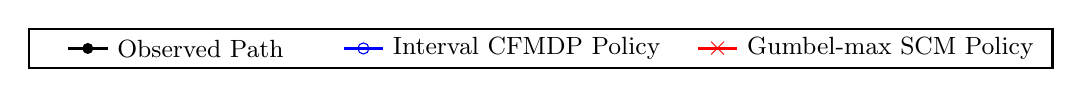
\begin{tikzpicture}[scale=1.0, every node/.style={scale=1.0}]
            \draw[thick, black] (-3, -0.25) rectangle (10, 0.25);
            %
            \draw[black, line width=1pt] (-2.5, 0.0) -- (-2,0.0);
            \fill[black] (-2.25,0.0) circle (2pt); %
            \node[right] at (-2,0.0) {\small Observed Path};
            
            %
            \draw[blue, line width=1pt] (1.0,0.0) -- (1.5,0.0);
            \node[draw=blue, circle, minimum size=4pt, inner sep=0pt] at (1.25,0.0) {}; %
            \node[right] at (1.5,0.0) {\small Interval CFMDP Policy};
            
            %
            \draw[red, line width=1pt] (5.5,0) -- (6,0);
            \node[red] at (5.75,0) {$\boldsymbol{\times}$}; %
            \node[right] at (6,0) {\small Gumbel-max SCM Policy};
        \end{tikzpicture}
    }\\
    %
    \subfigure[\footnotesize Lowest cumulative reward: Interval CFMDP ($312$), Gumbel-max SCM ($312$)]{%
        \resizebox{0.76\columnwidth}{!}{
             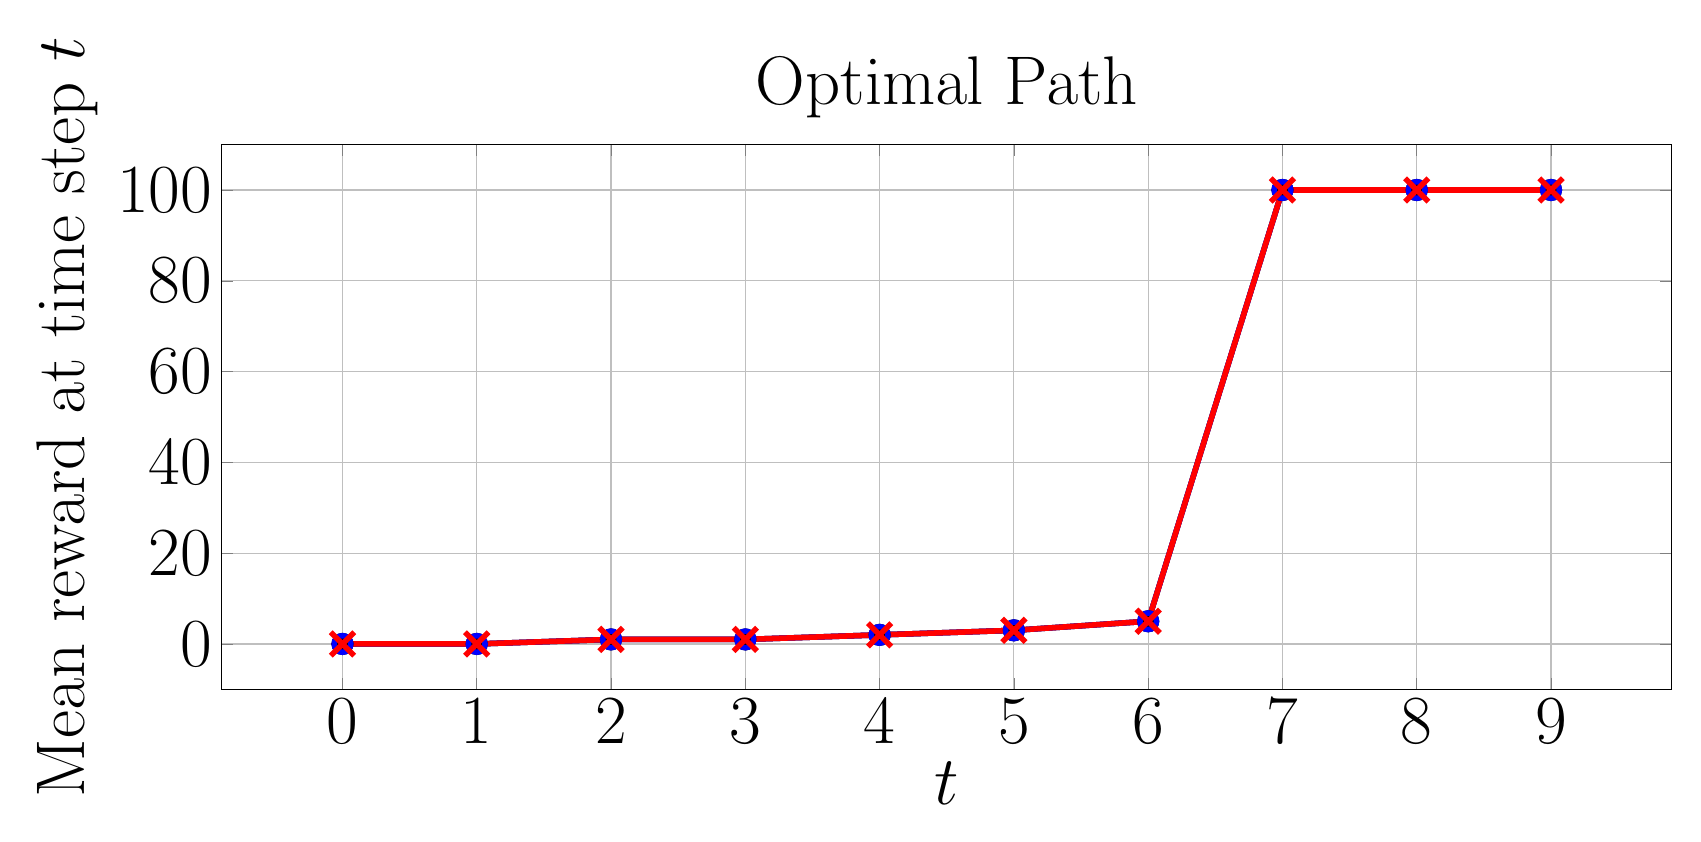
\begin{tikzpicture}
                \begin{axis}[
                    xlabel={$t$},
                    ylabel={Mean reward at time step $t$},
                    title={Optimal Path},
                    grid=both,
                    width=20cm, height=8.5cm,
                    every axis/.style={font=\Huge},
                    %
                ]
                \addplot[
                    color=black, %
                    mark=*, %
                    line width=2pt,
                    mark size=3pt,
                    error bars/.cd,
                    y dir=both, %
                    y explicit, %
                    error bar style={line width=1pt,solid},
                    error mark options={line width=1pt,mark size=4pt,rotate=90}
                ]
                coordinates {
                    (0, 0.0)  +- (0, 0.0)
                    (1, 0.0)  +- (0, 0.0) 
                    (2, 1.0)  +- (0, 0.0) 
                    (3, 1.0)  +- (0, 0.0)
                    (4, 2.0)  +- (0, 0.0)
                    (5, 3.0) +- (0, 0.0)
                    (6, 5.0) +- (0, 0.0)
                    (7, 100.0) +- (0, 0.0)
                    (8, 100.0) +- (0, 0.0)
                    (9, 100.0) +- (0, 0.0)
                };
                %
                \addplot[
                    color=blue, %
                    mark=o, %
                    line width=2pt,
                    mark size=3pt,
                    error bars/.cd,
                    y dir=both, %
                    y explicit, %
                    error bar style={line width=1pt,solid},
                    error mark options={line width=1pt,mark size=4pt,rotate=90}
                ]
                 coordinates {
                    (0, 0.0)  +- (0, 0.0)
                    (1, 0.0)  +- (0, 0.0) 
                    (2, 1.0)  +- (0, 0.0) 
                    (3, 1.0)  +- (0, 0.0)
                    (4, 2.0)  +- (0, 0.0)
                    (5, 3.0) +- (0, 0.0)
                    (6, 5.0) +- (0, 0.0)
                    (7, 100.0) +- (0, 0.0)
                    (8, 100.0) +- (0, 0.0)
                    (9, 100.0) +- (0, 0.0)
                };
                %
                \addplot[
                    color=red, %
                    mark=x, %
                    line width=2pt,
                    mark size=6pt,
                    error bars/.cd,
                    y dir=both, %
                    y explicit, %
                    error bar style={line width=1pt,solid},
                    error mark options={line width=1pt,mark size=4pt,rotate=90}
                ]
                coordinates {
                    (0, 0.0)  +- (0, 0.0)
                    (1, 0.0)  +- (0, 0.0) 
                    (2, 1.0)  +- (0, 0.0) 
                    (3, 1.0)  +- (0, 0.0)
                    (4, 2.0)  +- (0, 0.0)
                    (5, 3.0) +- (0, 0.0)
                    (6, 5.0) +- (0, 0.0)
                    (7, 100.0) +- (0, 0.0)
                    (8, 100.0) +- (0, 0.0)
                    (9, 100.0) +- (0, 0.0)
                };
                \end{axis}
            \end{tikzpicture}
         }
    }
    \hspace{1cm}
    \subfigure[\footnotesize Lowest cumulative reward: Interval CFMDP ($19$), Gumbel-max SCM ($-88$)]{%
         \resizebox{0.76\columnwidth}{!}{
            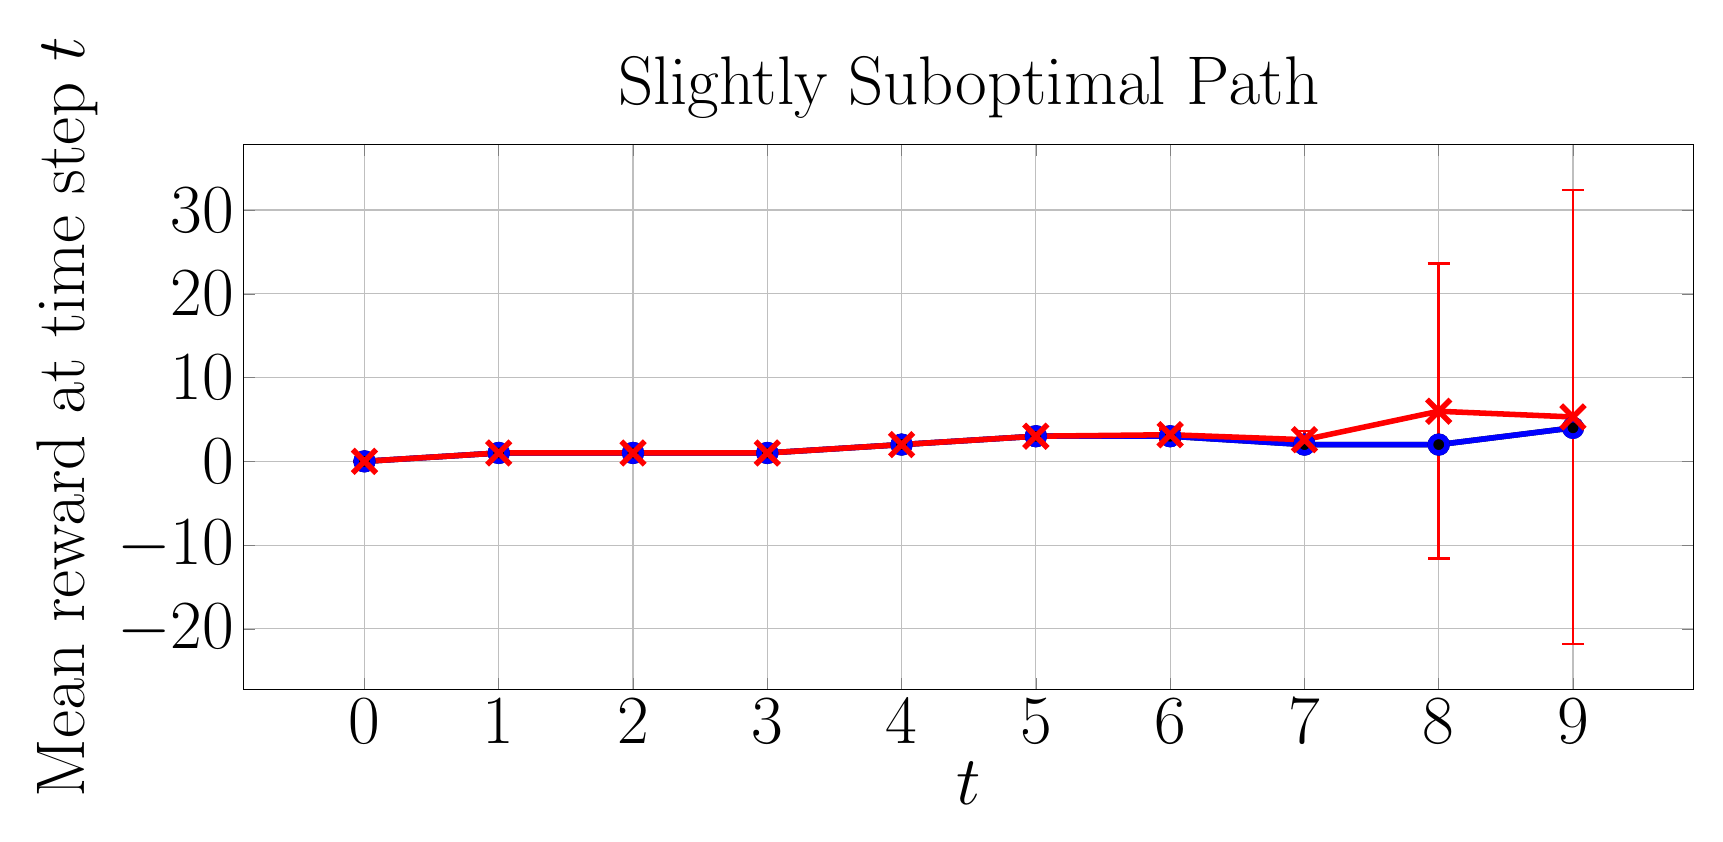
\begin{tikzpicture}
                \begin{axis}[
                    xlabel={$t$},
                    ylabel={Mean reward at time step $t$},
                    title={Slightly Suboptimal Path},
                    grid=both,
                    width=20cm, height=8.5cm,
                    every axis/.style={font=\Huge},
                    %
                ]
                \addplot[
                    color=black, %
                    mark=*, %
                    line width=2pt,
                    mark size=3pt,
                    error bars/.cd,
                    y dir=both, %
                    y explicit, %
                    error bar style={line width=1pt,solid},
                    error mark options={line width=1pt,mark size=4pt,rotate=90}
                ]
              coordinates {
                    (0, 0.0)  +- (0, 0.0)
                    (1, 1.0)  +- (0, 0.0) 
                    (2, 1.0)  +- (0, 0.0) 
                    (3, 1.0)  +- (0, 0.0)
                    (4, 2.0)  +- (0, 0.0)
                    (5, 3.0) +- (0, 0.0)
                    (6, 3.0) +- (0, 0.0)
                    (7, 2.0) +- (0, 0.0)
                    (8, 2.0) +- (0, 0.0)
                    (9, 4.0) +- (0, 0.0)
                };
                %
                \addplot[
                    color=blue, %
                    mark=o, %
                    line width=2pt,
                    mark size=3pt,
                    error bars/.cd,
                    y dir=both, %
                    y explicit, %
                    error bar style={line width=1pt,solid},
                    error mark options={line width=1pt,mark size=4pt,rotate=90}
                ]
              coordinates {
                    (0, 0.0)  +- (0, 0.0)
                    (1, 1.0)  +- (0, 0.0) 
                    (2, 1.0)  +- (0, 0.0) 
                    (3, 1.0)  +- (0, 0.0)
                    (4, 2.0)  +- (0, 0.0)
                    (5, 3.0) +- (0, 0.0)
                    (6, 3.0) +- (0, 0.0)
                    (7, 2.0) +- (0, 0.0)
                    (8, 2.0) +- (0, 0.0)
                    (9, 4.0) +- (0, 0.0)
                };
                %
                \addplot[
                    color=red, %
                    mark=x, %
                    line width=2pt,
                    mark size=6pt,
                    error bars/.cd,
                    y dir=both, %
                    y explicit, %
                    error bar style={line width=1pt,solid},
                    error mark options={line width=1pt,mark size=4pt,rotate=90}
                ]
                coordinates {
                    (0, 0.0)  +- (0, 0.0)
                    (1, 1.0)  +- (0, 0.0) 
                    (2, 1.0)  +- (0, 0.0) 
                    (3, 1.0)  +- (0, 0.0)
                    (4, 2.0)  += (0, 0.0)
                    (5, 3.0)  += (0, 0.0)
                    (6, 3.17847) += (0, 0.62606746) -= (0, 0.62606746)
                    (7, 2.5832885) += (0, 1.04598233) -= (0, 1.04598233)
                    (8, 5.978909) += (0, 17.60137623) -= (0, 17.60137623)
                    (9, 5.297059) += (0, 27.09227512) -= (0, 27.09227512)
                };
                \end{axis}
            \end{tikzpicture}
         }
    }\\[-1.5pt]
    \subfigure[\footnotesize Lowest cumulative reward: Interval CFMDP ($14$), Gumbel-max SCM ($-598$)]{%
         \resizebox{0.76\columnwidth}{!}{
             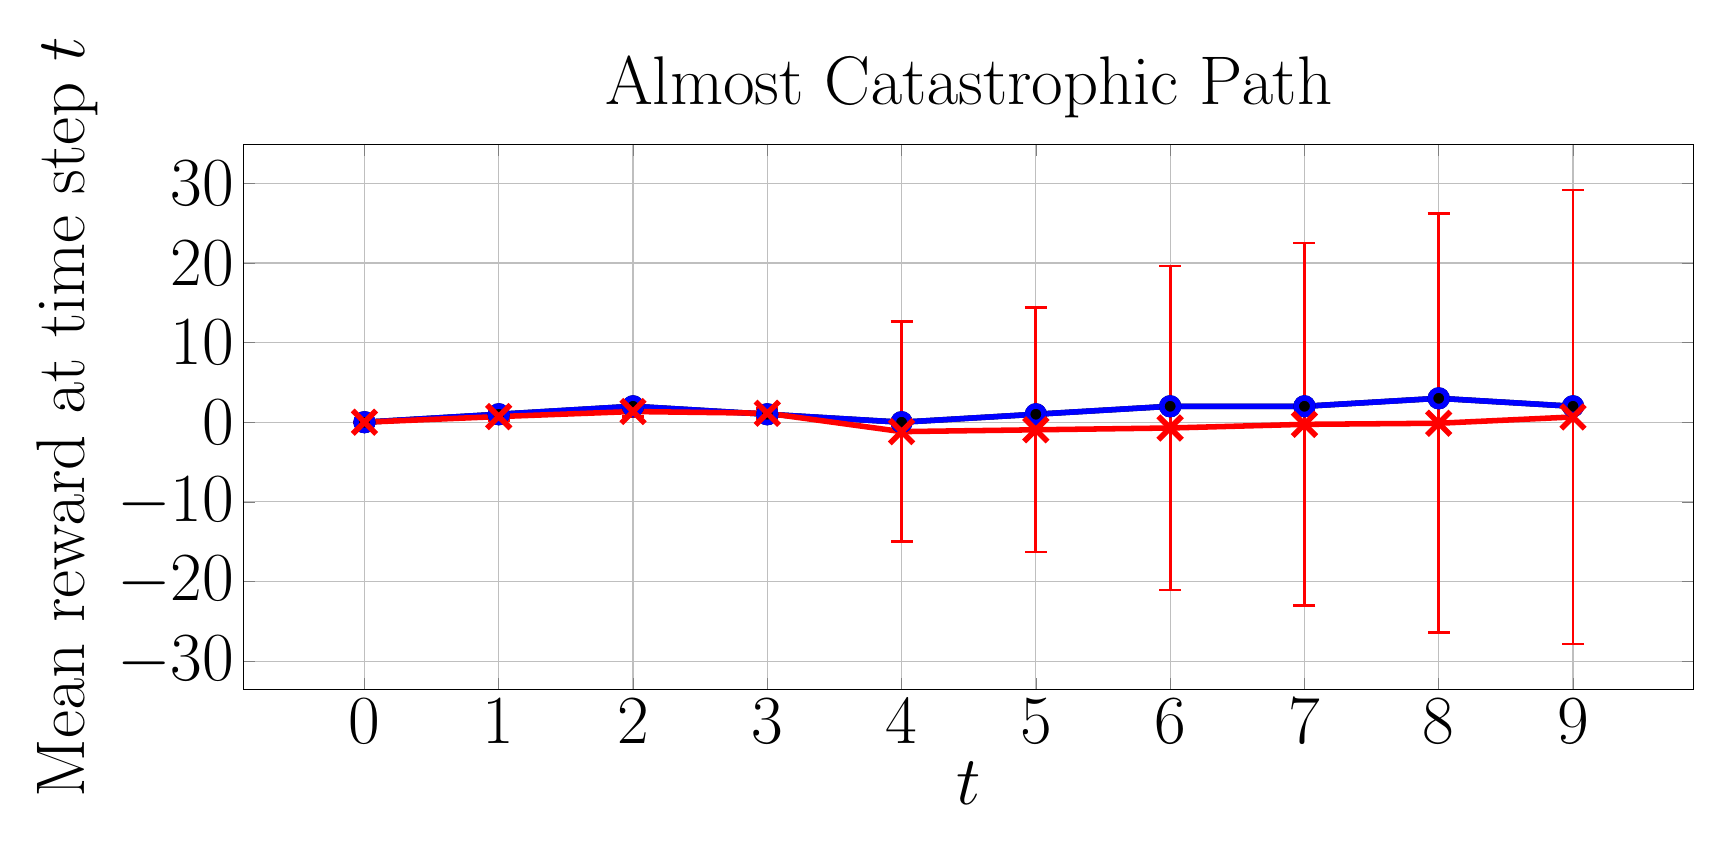
\begin{tikzpicture}
                \begin{axis}[
                    xlabel={$t$},
                    ylabel={Mean reward at time step $t$},
                    title={Almost Catastrophic Path},
                    grid=both,
                    width=20cm, height=8.5cm,
                    every axis/.style={font=\Huge},
                    %
                ]
                \addplot[
                    color=black, %
                    mark=*, %
                    line width=2pt,
                    mark size=3pt,
                    error bars/.cd,
                    y dir=both, %
                    y explicit, %
                    error bar style={line width=1pt,solid},
                    error mark options={line width=1pt,mark size=4pt,rotate=90}
                ]
                coordinates {
                    (0, 0.0)  +- (0, 0.0)
                    (1, 1.0)  +- (0, 0.0) 
                    (2, 2.0)  +- (0, 0.0) 
                    (3, 1.0)  +- (0, 0.0)
                    (4, 0.0)  +- (0, 0.0)
                    (5, 1.0) +- (0, 0.0)
                    (6, 2.0) +- (0, 0.0)
                    (7, 2.0) +- (0, 0.0)
                    (8, 3.0) +- (0, 0.0)
                    (9, 2.0) +- (0, 0.0)
                };
                %
                \addplot[
                    color=blue, %
                    mark=o, %
                    line width=2pt,
                    mark size=3pt,
                    error bars/.cd,
                    y dir=both, %
                    y explicit, %
                    error bar style={line width=1pt,solid},
                    error mark options={line width=1pt,mark size=4pt,rotate=90}
                ]
                coordinates {
                    (0, 0.0)  +- (0, 0.0)
                    (1, 1.0)  +- (0, 0.0) 
                    (2, 2.0)  +- (0, 0.0) 
                    (3, 1.0)  +- (0, 0.0)
                    (4, 0.0)  +- (0, 0.0)
                    (5, 1.0) +- (0, 0.0)
                    (6, 2.0) +- (0, 0.0)
                    (7, 2.0) +- (0, 0.0)
                    (8, 3.0) +- (0, 0.0)
                    (9, 2.0) +- (0, 0.0)
                };
                %
                \addplot[
                    color=red, %
                    mark=x, %
                    line width=2pt,
                    mark size=6pt,
                    error bars/.cd,
                    y dir=both, %
                    y explicit, %
                    error bar style={line width=1pt,solid},
                    error mark options={line width=1pt,mark size=4pt,rotate=90}
                ]
                coordinates {
                    (0, 0.0)  +- (0, 0.0)
                    (1, 0.7065655)  +- (0, 0.4553358) 
                    (2, 1.341673)  +- (0, 0.67091621) 
                    (3, 1.122926)  +- (0, 0.61281824)
                    (4, -1.1821935)  +- (0, 13.82444042)
                    (5, -0.952399)  +- (0, 15.35195457)
                    (6, -0.72672) +- (0, 20.33508414)
                    (7, -0.268983) +- (0, 22.77861454)
                    (8, -0.1310835) +- (0, 26.31013314)
                    (9, 0.65806) +- (0, 28.50670214)
                };
                %
            %
            %
            %
            %
            %
            %
            %
            %
            %
            %
            %
            %
            %
            %
            %
            %
            %
            %
                \end{axis}
            \end{tikzpicture}
         }
    }
    \hspace{1cm}
    \subfigure[\footnotesize Lowest cumulative reward: Interval CFMDP ($-698$), Gumbel-max SCM ($-698$)]{%
         \resizebox{0.76\columnwidth}{!}{
            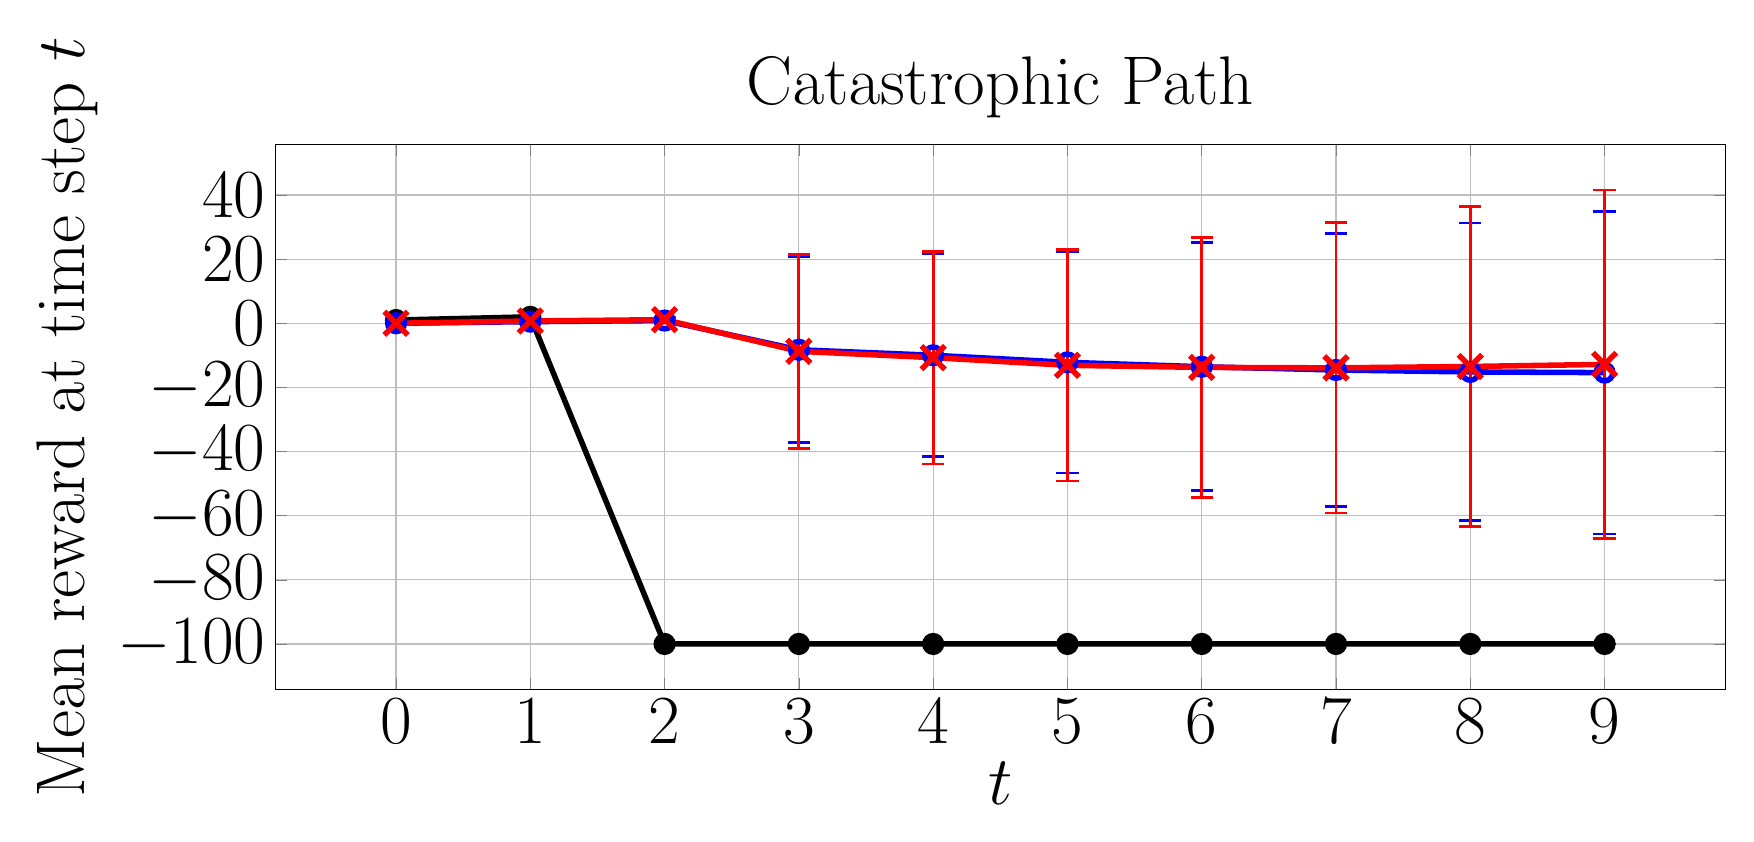
\begin{tikzpicture}
                \begin{axis}[
                    xlabel={$t$},
                    ylabel={Mean reward at time step $t$},
                    title={Catastrophic Path},
                    grid=both,
                    width=20cm, height=8.5cm,
                    every axis/.style={font=\Huge},
                    %
                ]
                \addplot[
                    color=black, %
                    mark=*, %
                    line width=2pt,
                    mark size=3pt,
                    error bars/.cd,
                    y dir=both, %
                    y explicit, %
                    error bar style={line width=1pt,solid},
                    error mark options={line width=1pt,mark size=4pt,rotate=90}
                ]
                coordinates {
                    (0, 1.0)  +- (0, 0.0)
                    (1, 2.0)  +- (0, 0.0) 
                    (2, -100.0)  +- (0, 0.0) 
                    (3, -100.0)  +- (0, 0.0)
                    (4, -100.0)  +- (0, 0.0)
                    (5, -100.0) +- (0, 0.0)
                    (6, -100.0) +- (0, 0.0)
                    (7, -100.0) +- (0, 0.0)
                    (8, -100.0) +- (0, 0.0)
                    (9, -100.0) +- (0, 0.0)
                };
                %
                \addplot[
                    color=blue, %
                    mark=o, %
                    line width=2pt,
                    mark size=3pt,
                    error bars/.cd,
                    y dir=both, %
                    y explicit, %
                    error bar style={line width=1pt,solid},
                    error mark options={line width=1pt,mark size=4pt,rotate=90}
                ]
                coordinates {
                    (0, 0.0)  +- (0, 0.0)
                    (1, 0.504814)  +- (0, 0.49997682) 
                    (2, 0.8439835)  +- (0, 0.76831917) 
                    (3, -8.2709165)  +- (0, 28.93656754)
                    (4, -9.981082)  +- (0, 31.66825363)
                    (5, -12.1776325) +- (0, 34.53463233)
                    (6, -13.556076) +- (0, 38.62845372)
                    (7, -14.574418) +- (0, 42.49603359)
                    (8, -15.1757075) +- (0, 46.41913968)
                    (9, -15.3900395) +- (0, 50.33563368)
                };
                %
                \addplot[
                    color=red, %
                    mark=x, %
                    line width=2pt,
                    mark size=6pt,
                    error bars/.cd,
                    y dir=both, %
                    y explicit, %
                    error bar style={line width=1pt,solid},
                    error mark options={line width=1pt,mark size=4pt,rotate=90}
                ]
                coordinates {
                    (0, 0.0)  +- (0, 0.0)
                    (1, 0.701873)  +- (0, 0.45743556) 
                    (2, 1.1227805)  +- (0, 0.73433129) 
                    (3, -8.7503255)  +- (0, 30.30257976)
                    (4, -10.722092)  +- (0, 33.17618589)
                    (5, -13.10721)  +- (0, 36.0648089)
                    (6, -13.7631645) +- (0, 40.56553451)
                    (7, -13.909043) +- (0, 45.23829402)
                    (8, -13.472517) +- (0, 49.96270296)
                    (9, -12.8278835) +- (0, 54.38618735)
                };
                %
            %
            %
            %
            %
            %
            %
            %
            %
            %
            %
            %
            %
            %
            %
            %
            %
            %
            %
                \end{axis}
            \end{tikzpicture}
         }
    }
    \caption{Average instant reward of CF paths induced by policies on GridWorld $p=0.4$.}
    \label{fig: reward p=0.4}
\end{figure*}

\subsection{Experimental Setup}
To compare policy performance, we measure the average rewards of counterfactual paths induced by our policy and the Gumbel-max policy by uniformly sampling $200$ counterfactual MDPs from the ICFMDP and generating $10,000$ counterfactual paths over each sampled CFMDP. \jl{Since the interval CFMDP depends on the observed path, we select $4$  paths of varying optimality to evaluate how the observed path impacts the performance of both policies: an optimal path, a slightly suboptimal path that could reach the optimal reward with a few changes, a catastrophic path that enters a catastrophic, terminal state with low reward, and an almost catastrophic path that was close to entering a catastrophic state.} When measuring the average probability bound widths and execution time needed to generate the ICFMDPs, we averaged over $20$ randomly generated observed paths
\footnote{Further training details are provided in Appendix \ref{app: training details}, and the code is provided at \href{https://github.com/ddv-lab/robust-cf-inference-in-MDPs}{https://github.com/ddv-lab/robust-cf-inference-in-MDPs}
%
%
.}.

\subsection{GridWorld}
\jl{The GridWorld MDP is a $4 \times 4$ grid where an agent must navigate from the top-left corner to the goal state in the bottom-right corner, avoiding a dangerous terminal state in the centre. At each time step, the agent can move up, down, left, or right, but there is a small probability (controlled by hyper-parameter $p$) of moving in an unintended direction. As the agent nears the goal, the reward for each state increases, culminating in a reward of $+100$ for reaching the goal. Entering the dangerous state results in a penalty of $-100$. We use two versions of GridWorld: a less stochastic version with $p=0.9$ (i.e., $90$\% chance of moving in the chosen direction) and a more stochastic version with $p=0.4$.}

\paragraph{GridWorld ($p=0.9$)}
When $p=0.9$, the counterfactual probability bounds are typically narrow (see Table \ref{tab:nonzero_probs} for average measurements). Consequently, as shown in Figure \ref{fig: reward p=0.9}, both policies are nearly identical and perform similarly well across the optimal, slightly suboptimal, and catastrophic paths.
%
However, for the almost catastrophic path, the interval CFMDP path is more conservative and follows the observed path more closely (as this is where the probability bounds are narrowest), which typically requires one additional step to reach the goal state than the Gumbel-max SCM policy.
%

\paragraph{GridWorld ($p=0.4$)}
\jl{When $p=0.4$, the GridWorld environment becomes more uncertain, increasing the risk of entering the dangerous state even if correct actions are chosen. Thus, as shown in Figure \ref{fig: reward p=0.4}, the interval CFMDP policy adopts a more conservative approach, avoiding deviation from the observed policy if it cannot guarantee higher counterfactual rewards (see the slightly suboptimal and almost catastrophic paths), whereas the Gumbel-max SCM is inconsistent: it can yield higher rewards, but also much lower rewards, reflected in the wide error bars.} For the catastrophic path, both policies must deviate from the observed path to achieve a higher reward and, in this case, perform similarly.
%
%
%
%
\subsection{Sepsis}
The Sepsis MDP \citep{oberst2019counterfactual} simulates trajectories of Sepsis patients. Each state consists of four vital signs (heart rate, blood pressure, oxygen concentration, and glucose levels), categorised as low, normal, or high.
and three treatments that can be toggled on/off at each time step (8 actions in total). Unlike \citet{oberst2019counterfactual}, we scale rewards based on the number of out-of-range vital signs, between $-1000$ (patient dies) and $1000$ (patient discharged). \jl{Like the GridWorld $p=0.4$ experiment, the Sepsis MDP is highly uncertain, as many states are equally likely to lead to optimal and poor outcomes. Thus, as shown in Figure \ref{fig: reward sepsis}, both policies follow the observed optimal and almost catastrophic paths to guarantee rewards are no worse than the observation.} However, improving the catastrophic path requires deviating from the observation. Here, the Gumbel-max SCM policy, on average, performs better than the interval CFMDP policy. But, since both policies have lower bounds clipped at $-1000$, neither policy reliably improves over the observation. In contrast, for the slightly suboptimal path, the interval CFMDP policy performs significantly better, shown by its higher lower bounds. 
Moreover, in these two cases, the worst-case counterfactual path generated by the interval CFMDP policy is better than that of the Gumbel-max SCM policy,
indicating its greater robustness.
%
\begin{figure*}
    \centering
     \resizebox{0.6\textwidth}{!}{
        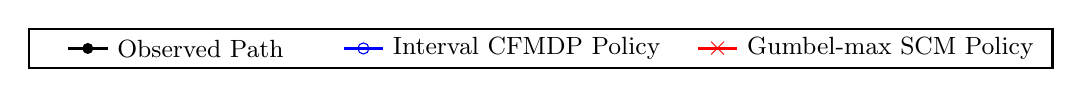
\begin{tikzpicture}[scale=1.0, every node/.style={scale=1.0}]
            \draw[thick, black] (-3, -0.25) rectangle (10, 0.25);
            %
            \draw[black, line width=1pt] (-2.5, 0.0) -- (-2,0.0);
            \fill[black] (-2.25,0.0) circle (2pt); %
            \node[right] at (-2,0.0) {\small Observed Path};
            
            %
            \draw[blue, line width=1pt] (1.0,0.0) -- (1.5,0.0);
            \node[draw=blue, circle, minimum size=4pt, inner sep=0pt] at (1.25,0.0) {}; %
            \node[right] at (1.5,0.0) {\small Interval CFMDP Policy};
            
            %
            \draw[red, line width=1pt] (5.5,0) -- (6,0);
            \node[red] at (5.75,0) {$\boldsymbol{\times}$}; %
            \node[right] at (6,0) {\small Gumbel-max SCM Policy};
        \end{tikzpicture}
    }\\
    \subfigure[\footnotesize Lowest cumulative reward: Interval CFMDP ($8000$), Gumbel-max SCM ($8000$)]{%
         \resizebox{0.76\columnwidth}{!}{
             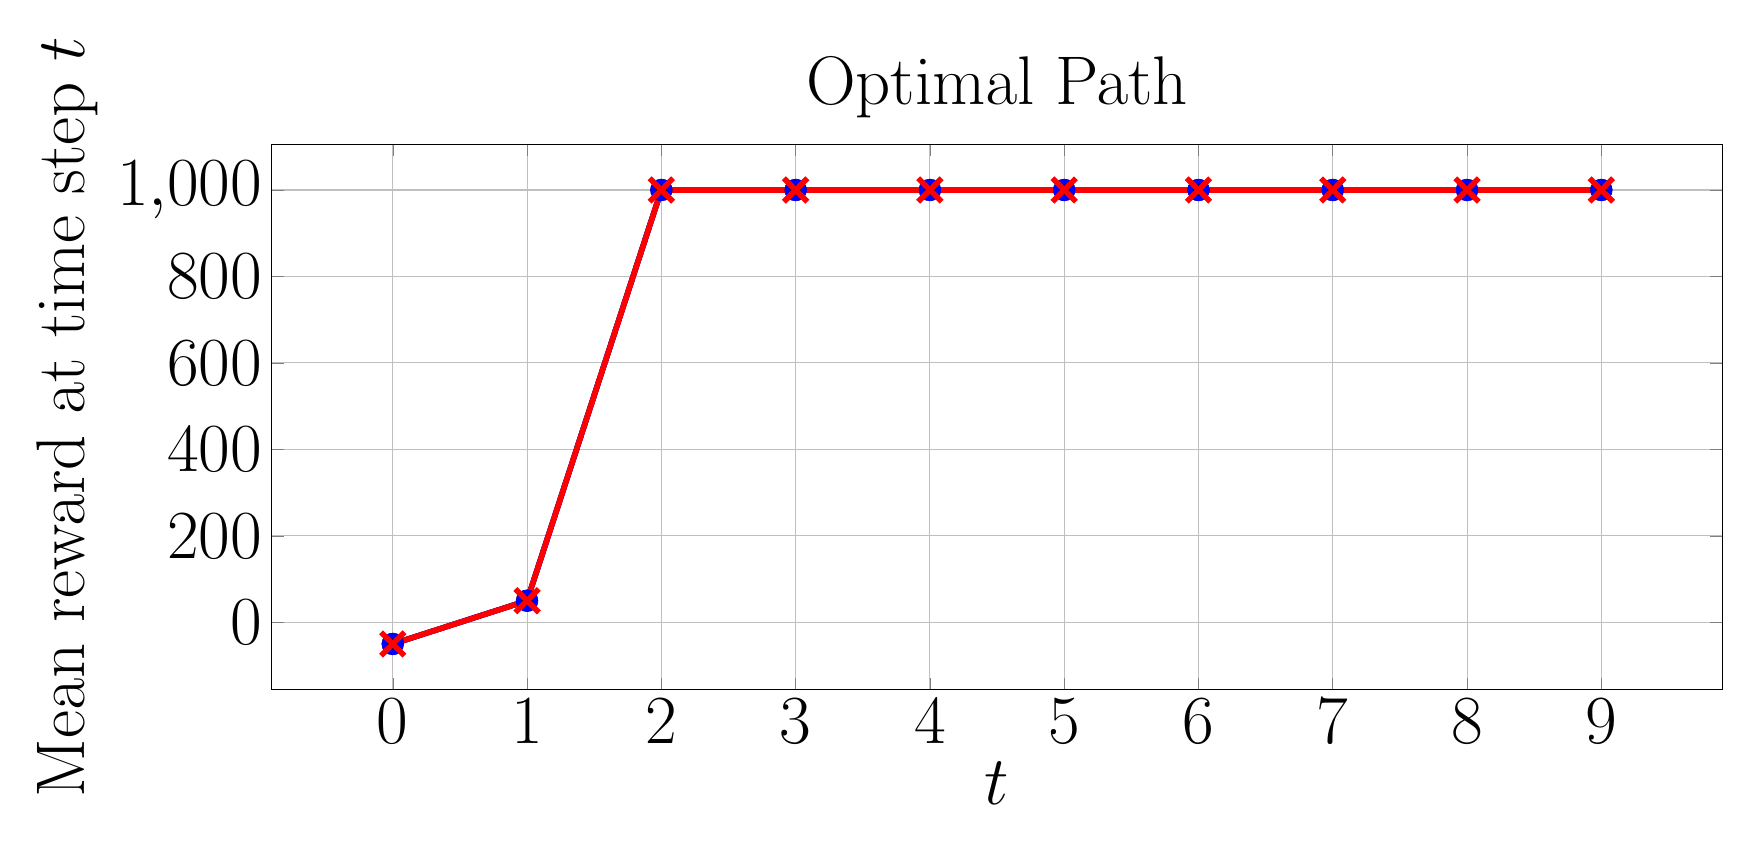
\begin{tikzpicture}
                \begin{axis}[
                    xlabel={$t$},
                    ylabel={Mean reward at time step $t$},
                    title={Optimal Path},
                    grid=both,
                    width=20cm, height=8.5cm,
                    every axis/.style={font=\Huge},
                    %
                ]
                \addplot[
                    color=black, %
                    mark=*, %
                    line width=2pt,
                    mark size=3pt,
                ]
                coordinates {
                    (0, -50.0)
                    (1, 50.0)
                    (2, 1000.0)
                    (3, 1000.0)
                    (4, 1000.0)
                    (5, 1000.0)
                    (6, 1000.0)
                    (7, 1000.0)
                    (8, 1000.0)
                    (9, 1000.0)
                };
                %
                \addplot[
                    color=blue, %
                    mark=o, %
                    line width=2pt,
                    mark size=3pt,
                    error bars/.cd,
                    y dir=both, %
                    y explicit, %
                    error bar style={line width=1pt,solid},
                    error mark options={line width=1pt,mark size=4pt,rotate=90}
                ]
                coordinates {
                    (0, -50.0)  +- (0, 0.0)
                    (1, 50.0)  +- (0, 0.0) 
                    (2, 1000.0)  +- (0, 0.0) 
                    (3, 1000.0)  +- (0, 0.0)
                    (4, 1000.0)  +- (0, 0.0)
                    (5, 1000.0) +- (0, 0.0)
                    (6, 1000.0) +- (0, 0.0)
                    (7, 1000.0) +- (0, 0.0)
                    (8, 1000.0) +- (0, 0.0)
                    (9, 1000.0) +- (0, 0.0)
                };
                %
                \addplot[
                    color=red, %
                    mark=x, %
                    line width=2pt,
                    mark size=6pt,
                    error bars/.cd,
                    y dir=both, %
                    y explicit, %
                    error bar style={line width=1pt,solid},
                    error mark options={line width=1pt,mark size=4pt,rotate=90}
                ]
                coordinates {
                    (0, -50.0)  +- (0, 0.0)
                    (1, 50.0)  +- (0, 0.0) 
                    (2, 1000.0)  +- (0, 0.0) 
                    (3, 1000.0)  +- (0, 0.0)
                    (4, 1000.0)  +- (0, 0.0)
                    (5, 1000.0) +- (0, 0.0)
                    (6, 1000.0) +- (0, 0.0)
                    (7, 1000.0) +- (0, 0.0)
                    (8, 1000.0) +- (0, 0.0)
                    (9, 1000.0) +- (0, 0.0)
                };
                %
                \end{axis}
            \end{tikzpicture}
         }
    }
    \hspace{1cm}
    \subfigure[\footnotesize Lowest cumulative reward: Interval CFMDP ($-5980$), Gumbel-max SCM ($-8000$)]{%
         \resizebox{0.76\columnwidth}{!}{
            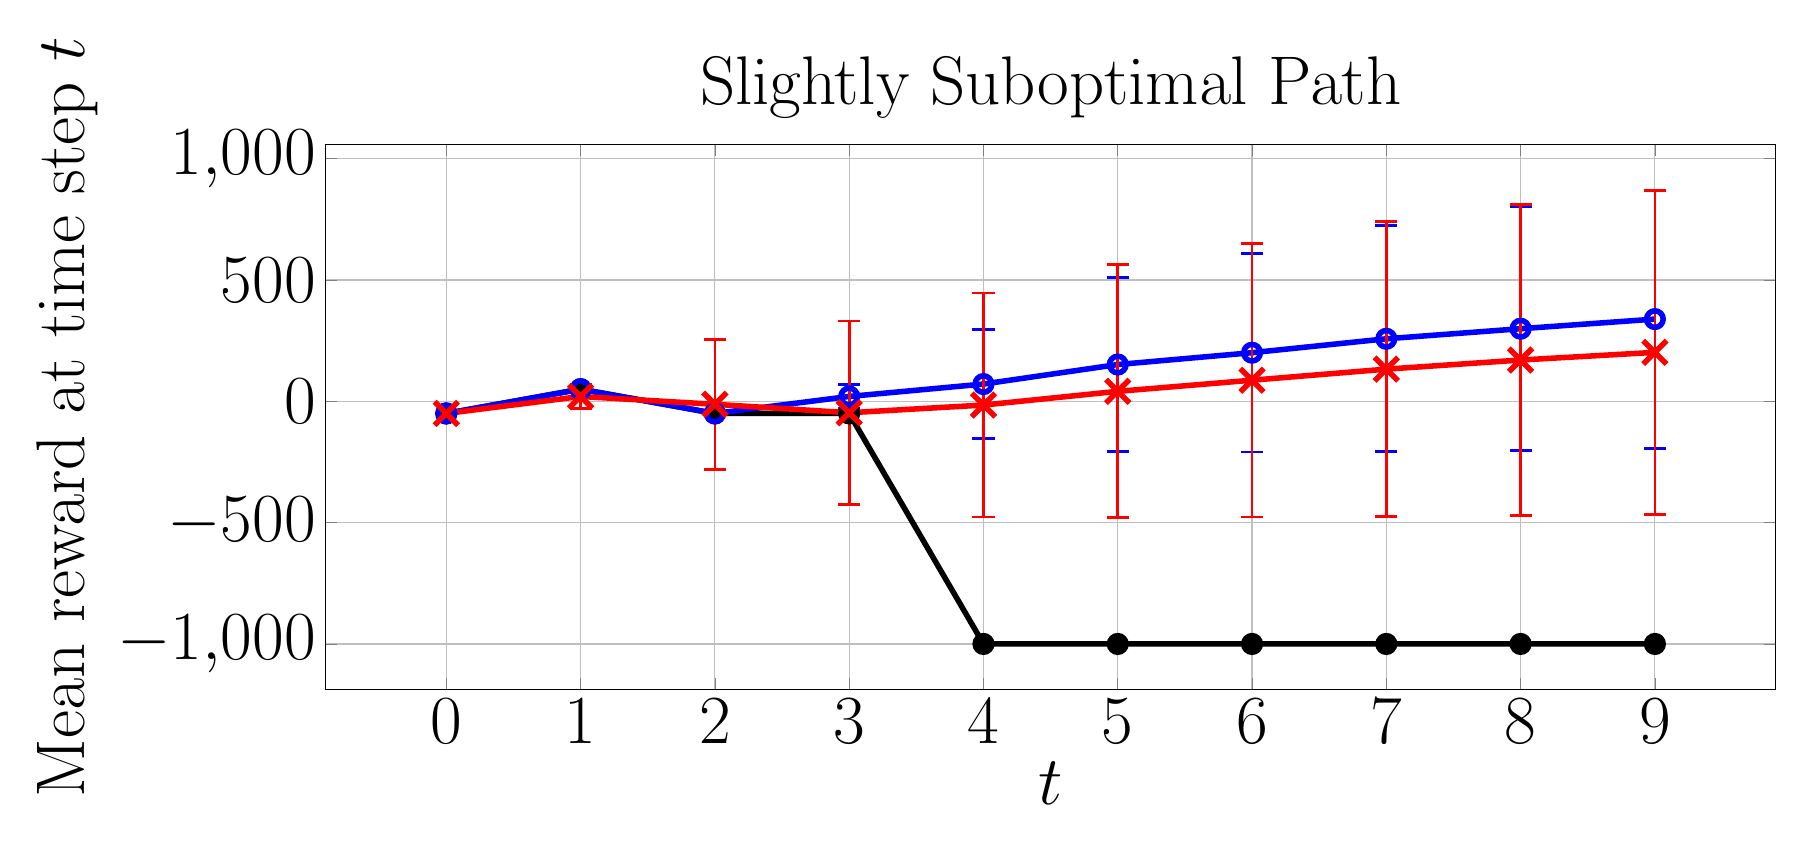
\begin{tikzpicture}
                \begin{axis}[
                    xlabel={$t$},
                    ylabel={Mean reward at time step $t$},
                    title={Slightly Suboptimal Path},
                    grid=both,
                    width=20cm, height=8.5cm,
                    every axis/.style={font=\Huge},
                    %
                ]
               \addplot[
                    color=black, %
                    mark=*, %
                    line width=2pt,
                    mark size=3pt,
                ]
                coordinates {
                    (0, -50.0)
                    (1, 50.0)
                    (2, -50.0)
                    (3, -50.0)
                    (4, -1000.0)
                    (5, -1000.0)
                    (6, -1000.0)
                    (7, -1000.0)
                    (8, -1000.0)
                    (9, -1000.0)
                };
                %
                \addplot[
                    color=blue, %
                    mark=o, %
                    line width=2pt,
                    mark size=3pt,
                    error bars/.cd,
                    y dir=both, %
                    y explicit, %
                    error bar style={line width=1pt,solid},
                    error mark options={line width=1pt,mark size=4pt,rotate=90}
                ]
                coordinates {
                    (0, -50.0)  +- (0, 0.0)
                    (1, 50.0)  +- (0, 0.0) 
                    (2, -50.0)  +- (0, 0.0) 
                    (3, 20.0631)  +- (0, 49.97539413)
                    (4, 71.206585)  +- (0, 226.02033693)
                    (5, 151.60797) +- (0, 359.23292559)
                    (6, 200.40593) +- (0, 408.86185176)
                    (7, 257.77948) +- (0, 466.10372804)
                    (8, 299.237465) +- (0, 501.82579506)
                    (9, 338.9129) +- (0, 532.06124996)
                };
                %
                \addplot[
                    color=red, %
                    mark=x, %
                    line width=2pt,
                    mark size=6pt,
                    error bars/.cd,
                    y dir=both, %
                    y explicit, %
                    error bar style={line width=1pt,solid},
                    error mark options={line width=1pt,mark size=4pt,rotate=90}
                ]
                coordinates {
                    (0, -50.0)  +- (0, 0.0)
                    (1, 20.00736)  +- (0, 49.99786741) 
                    (2, -12.282865)  +- (0, 267.598755) 
                    (3, -47.125995)  +- (0, 378.41755832)
                    (4, -15.381965)  +- (0, 461.77616558)
                    (5, 41.15459) +- (0, 521.53189262)
                    (6, 87.01595) +- (0, 564.22243126 )
                    (7, 132.62376) +- (0, 607.31338037)
                    (8, 170.168145) +- (0, 641.48013693)
                    (9, 201.813135) +- (0, 667.29441777)
                };
                %
                %
                %
                %
                %
                %
                %
                %
                %
                %
                %
                %
                %
                %
                %
                %
                %
                %
                %
                \end{axis}
            \end{tikzpicture}
         }
    }\\[-1.5pt]
    \subfigure[\footnotesize Lowest cumulative reward: Interval CFMDP ($100$), Gumbel-max SCM ($100$)]{%
         \resizebox{0.76\columnwidth}{!}{
             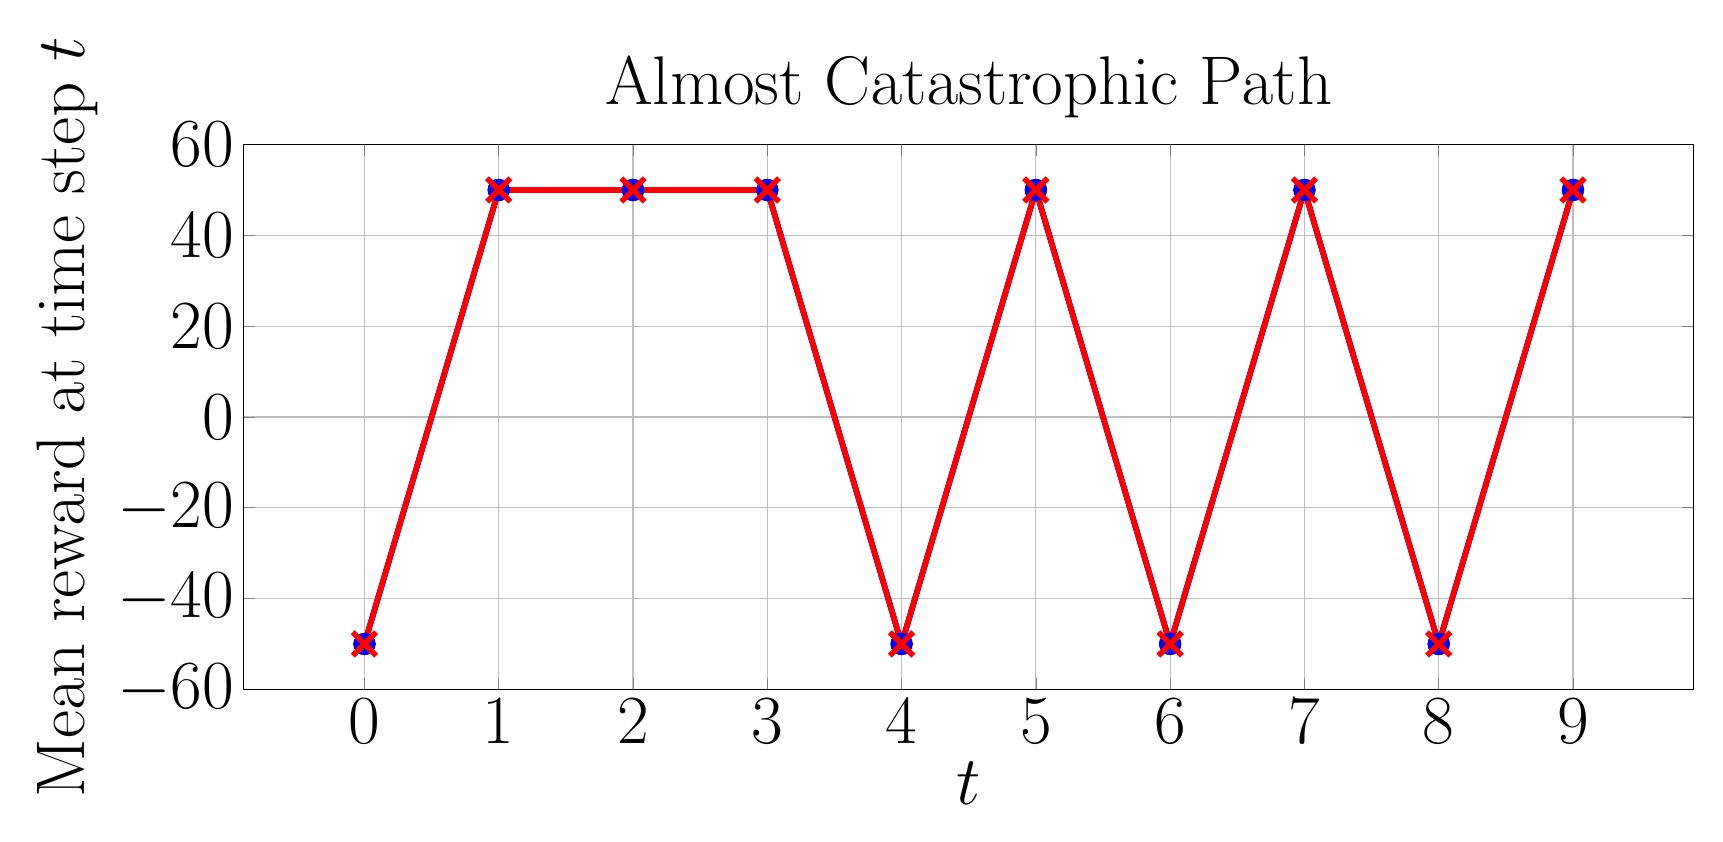
\begin{tikzpicture}
                \begin{axis}[
                    xlabel={$t$},
                    ylabel={Mean reward at time step $t$},
                    title={Almost Catastrophic Path},
                    grid=both,
                    every axis/.style={font=\Huge},
                    width=20cm, height=8.5cm,
                    %
                ]
               \addplot[
                    color=black, %
                    mark=*, %
                    line width=2pt,
                    mark size=3pt,
                ]
                coordinates {
                    (0, -50.0)
                    (1, 50.0)
                    (2, 50.0)
                    (3, 50.0)
                    (4, -50.0)
                    (5, 50.0)
                    (6, -50.0)
                    (7, 50.0)
                    (8, -50.0)
                    (9, 50.0)
                };
                %
                %
                \addplot[
                    color=blue, %
                    mark=o, %
                    line width=2pt,
                    mark size=3pt,
                    error bars/.cd,
                    y dir=both, %
                    y explicit, %
                    error bar style={line width=1pt,solid},
                    error mark options={line width=1pt,mark size=4pt,rotate=90}
                ]
                coordinates {
                    (0, -50.0)  +- (0, 0.0)
                    (1, 50.0)  +- (0, 0.0) 
                    (2, 50.0)  +- (0, 0.0) 
                    (3, 50.0)  +- (0, 0.0)
                    (4, -50.0)  +- (0, 0.0)
                    (5, 50.0) +- (0, 0.0)
                    (6, -50.0) +- (0, 0.0)
                    (7, 50.0) +- (0, 0.0)
                    (8, -50.0) +- (0, 0.0)
                    (9, 50.0) +- (0, 0.0)
                };
                %
                \addplot[
                    color=red, %
                    mark=x, %
                    line width=2pt,
                    mark size=6pt,
                    error bars/.cd,
                    y dir=both, %
                    y explicit, %
                    error bar style={line width=1pt,solid},
                    error mark options={line width=1pt,mark size=4pt,rotate=90}
                ]
                coordinates {
                    (0, -50.0)  +- (0, 0.0)
                    (1, 50.0)  +- (0, 0.0) 
                    (2, 50.0)  +- (0, 0.0) 
                    (3, 50.0)  +- (0, 0.0)
                    (4, -50.0)  +- (0, 0.0)
                    (5, 50.0) +- (0, 0.0)
                    (6, -50.0) +- (0, 0.0)
                    (7, 50.0) +- (0, 0.0)
                    (8, -50.0) +- (0, 0.0)
                    (9, 50.0) +- (0, 0.0)
                };
                %
                %
                %
                %
                %
                %
                %
                %
                %
                %
                %
                %
                %
                %
                %
                %
                %
                %
                %
                \end{axis}
            \end{tikzpicture}
         }
    }
    \hspace{1cm}
    \subfigure[\footnotesize Lowest cumulative reward: Interval CFMDP ($-7150$), Gumbel-max SCM ($-9050$)]{%
         \resizebox{0.76\columnwidth}{!}{
            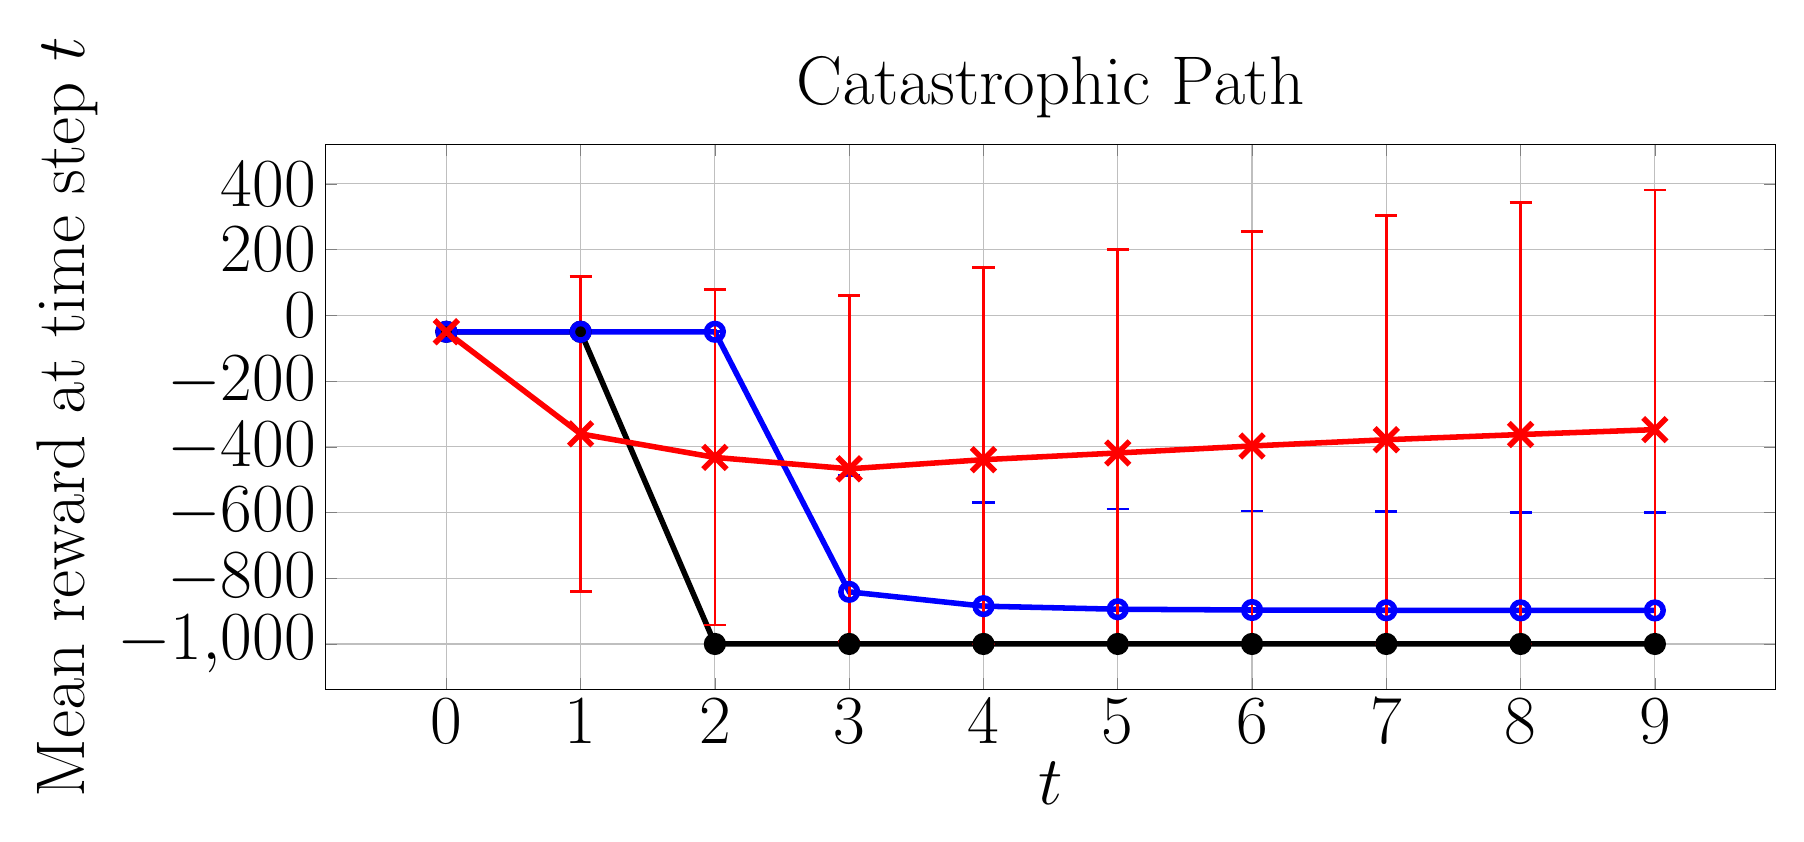
\begin{tikzpicture}
                \begin{axis}[
                    xlabel={$t$},
                    ylabel={Mean reward at time step $t$},
                    title={Catastrophic Path},
                    grid=both,
                    width=20cm, height=8.5cm,
                    every axis/.style={font=\Huge},
                    %
                ]
               \addplot[
                    color=black, %
                    mark=*, %
                    line width=2pt,
                    mark size=3pt,
                ]
                coordinates {
                    (0, -50.0)
                    (1, -50.0)
                    (2, -1000.0)
                    (3, -1000.0)
                    (4, -1000.0)
                    (5, -1000.0)
                    (6, -1000.0)
                    (7, -1000.0)
                    (8, -1000.0)
                    (9, -1000.0)
                };
                %
                %
                \addplot[
                    color=blue, %
                    mark=o, %
                    line width=2pt,
                    mark size=3pt,
                    error bars/.cd,
                    y dir=both, %
                    y explicit, %
                    error bar style={line width=1pt,solid},
                    error mark options={line width=1pt,mark size=4pt,rotate=90}
                ]
                coordinates {
                    (0, -50.0)  +- (0, 0.0)
                    (1, -50.0)  +- (0, 0.0) 
                    (2, -50.0)  +- (0, 0.0) 
                    (3, -841.440725)  += (0, 354.24605512) -= (0, 158.559275)
                    (4, -884.98225)  += (0, 315.37519669) -= (0, 115.01775)
                    (5, -894.330425) += (0, 304.88572805) -= (0, 105.669575)
                    (6, -896.696175) += (0, 301.19954514) -= (0, 103.303825)
                    (7, -897.4635) += (0, 299.61791279) -= (0, 102.5365)
                    (8, -897.77595) += (0, 298.80392585) -= (0, 102.22405)
                    (9, -897.942975) += (0, 298.32920557) -= (0, 102.057025)
                };
                %
                \addplot[
                    color=red, %
                    mark=x, %
                    line width=2pt,
                    mark size=6pt,
                    error bars/.cd,
                    y dir=both, %
                    y explicit, %
                    error bar style={line width=1pt,solid},
                    error mark options={line width=1pt,mark size=4pt,rotate=90}
                ]
            coordinates {
                    (0, -50.0)  +- (0, 0.0)
                    (1, -360.675265)  +- (0, 479.39812699) 
                    (2, -432.27629)  +- (0, 510.38620897) 
                    (3, -467.029545)  += (0, 526.36009628) -= (0, 526.36009628)
                    (4, -439.17429)  += (0, 583.96638919) -= (0, 560.82571)
                    (5, -418.82704) += (0, 618.43027478) -= (0, 581.17296)
                    (6, -397.464895) += (0, 652.67322574) -= (0, 602.535105)
                    (7, -378.49052) += (0, 682.85407033) -= (0, 621.50948)
                    (8, -362.654195) += (0, 707.01412023) -= (0, 637.345805)
                    (9, -347.737935) += (0, 729.29076479) -= (0, 652.262065)
                };
                %
                %
                %
                %
                %
                %
                %
                %
                %
                %
                %
                %
                %
                %
                %
                %
                %
                %
                %
                \end{axis}
            \end{tikzpicture}
         }
    }
    \caption{Average instant reward of CF paths induced by policies on Sepsis.}
    \label{fig: reward sepsis}
\end{figure*}

%
%
%
\subsection{Interval CFMDP Bounds}
%
%
Table \ref{tab:nonzero_probs} presents the mean counterfactual probability bound widths (excluding transitions where the upper bound is $0$) for each MDP, averaged over 20 observed paths. We compare the bounds under counterfactual stability (CS) and monotonicity (M) assumptions, CS alone, and no assumptions. This shows that the assumptions marginally reduce the bound widths, indicating the assumptions tighten the bounds without excluding too many causal models, as intended.
\renewcommand{\arraystretch}{1}

\begin{table}
\centering
\caption{Mean width of counterfactual probability bounds}
\resizebox{0.8\columnwidth}{!}{%
\begin{tabular}{|c|c|c|c|}
\hline
\multirow{2}{*}{\textbf{Environment}} & \multicolumn{3}{c|}{\textbf{Assumptions}} \\ \cline{2-4}
 & \textbf{CS + M} & \textbf{CS} & \textbf{None\tablefootnote{\jl{Equivalent to \citet{li2024probabilities}'s bounds (see Section \ref{sec: equivalence with Li}).}}} \\ \hline
\textbf{GridWorld} ($p=0.9$) & 0.0817 & 0.0977 & 0.100 \\ \hline
\textbf{GridWorld} ($p=0.4$) & 0.552  & 0.638  & 0.646 \\ \hline
\textbf{Sepsis} & 0.138 & 0.140 & 0.140 \\ \hline
\end{tabular}
}
\label{tab:nonzero_probs}
\end{table}


\subsection{Execution Times}
Table \ref{tab: times} compares the average time needed to generate the interval CFMDP vs.\ the Gumbel-max SCM CFMDP for 20 observations.
The GridWorld algorithms were run single-threaded, while the Sepsis experiments were run in parallel.
Generating the interval CFMDP is significantly faster as it uses exact analytical bounds, whereas the Gumbel-max CFMDP requires sampling from the Gumbel distribution to estimate counterfactual transition probabilities. \jl{Since constructing the counterfactual MDP models is the main bottleneck in both approaches, ours is more efficient overall and suitable for larger MDPs.}
\begin{table}
\centering
\caption{Mean execution time to generate CFMDPs}
\resizebox{0.99\columnwidth}{!}{%
\begin{tabular}{|c|c|c|}
\hline
\multirow{2}{*}{\textbf{Environment}} & \multicolumn{2}{c|}{\textbf{Mean Execution Time (s)}} \\ \cline{2-3} 
                                      & \textbf{Interval CFMDP} & \textbf{Gumbel-max CFMDP} \\ \hline
\textbf{GridWorld ($p=0.9$) }                  & 0.261                   & 56.1                      \\ \hline
\textbf{GridWorld ($p=0.4$)  }                 & 0.336                   & 54.5                      \\ \hline
\textbf{Sepsis}                                 & 688                     & 2940                      \\ \hline
\end{tabular}%
}
\label{tab: times}
\end{table}


\subsubsection{Results}
\section{Analysis}
\label{sec:analysis}
In the following sections, we will analyze European type approval regulation\footnote{Strictly speaking, the German enabling act (AFGBV) does not regulate type-approval, but how test \& operating permits are issued for SAE-Level-4 systems. Type-approval regulation for SAE-Level-3 systems follows UN Regulation No. 157 (UN-ECE-ALKS) \parencite{un157}.} regarding the underlying notions of ``safety'' and ``risk''.
We will classify these notions according to their absolute or relative character, underlying risk sources, or underlying concepts of harm.

\subsection{Classification of Safety Notions}
\label{sec:safety-notions}
We will refer to \emph{absolute} notions of safety as conceptualizations that assume the complete absence of any kind of risk.
Opposed to this, \emph{relative} notions of safety are based on a conceptualization that specifically includes risk acceptance criteria, e.g., in terms of ``tolerable'' risk or ``sufficient'' safety.

For classifying notions of safety by their underlying risk (or rather ``hazard'') sources, and different concepts of harm, \Cref{fig:hazard-sources} provides an overview of our reasoning, which is closely in line with the argumentation provided by Waymo in \parencite{favaro2023}.
We prefer ``hazard sources'' over ``risk sources'', as a risk must always be related to a \emph{cause} or \emph{source of harm} (i.e., a hazard \parencite[p.~1, def. 3.2]{iso51}).
Without a concrete (scenario) context that the system is operating in, a hazard is \emph{latent}: E.g., when operating in public traffic, there is a fundamental possibility that a \emph{collision with a pedestrian} leads to (physical) harm for that pedestrian. 
However, only if an automated vehicle shows (potentially) hazardous behavior (e.g., not decelerating properly) \emph{and} is located near a pedestrian (context), the hazard is instantiated and leads to a hazardous event.
\begin{figure*}
    \includeimg[width=.9\textwidth]{hazard-sources0.pdf}
    \caption{Graphical summary of a taxonomy of risk related to automated vehicles, extended based on ISO 21448 (\parencite{iso21448}) and \parencite{favaro2023}. Top: Causal chain from hazard sources to actual harm; bottom: summary of the individual elements' contributions to a resulting risk. Graphic translated from \parencite{nolte2024} \label{fig:hazard-sources}}
\end{figure*}
If the hazardous event cannot be mitigated or controlled, we see a loss event in which the pedestrian's health is harmed.
Note that this hypothetical chain of events is summarized in the definition of risk:
The probability of occurrence of harm is determined by a) the frequency with which hazard sources manifest, b) the time for which the system operates in a context that exposes the possibility of harm, and c) by the probability with which a hazardous event can be controlled.
A risk can then be determined as a function of the probability of harm and the severity of the harm potentially inflicted on the pedestrian.

In the following, we will apply this general model to introduce different types of hazard sources and also different types of harm.
\cref{fig:hazard-sources} shows two distinct hazard sources, i.e., functional insufficiencies and E/E-failures that can lead to hazardous behavior.
ISO~21488 \parencite{iso21448} defines functional insufficiencies as insufficiencies that stem from an incomplete or faulty system specification (specification insufficiencies).
In addition, the standard considers insufficiencies that stem from insufficient technical capability to operate inside the targeted Operational Design Domain (performance insufficiencies).
Functional insufficiencies are related to the ``Safety of the Intended Functionality (SOTIF)'' (according to ISO~21448), ``Behavioral Safety'' (according to Waymo \parencite{waymo2018}), or ``Operational Safety'' (according to UN Regulation No. 157 \parencite{un157}).
E/E-Failures are related to classic functional safety and are covered exhaustively by ISO~26262 \parencite{iso2018}.
Additional hazard sources can, e.g., be related to malicious security attacks (ISO~21434), or even to mechanical failures that should be covered (in the US) in the Federal Motor Vehicle Safety Standards (FMVSS).

For the classification of notions of safety by the related harm, in \parencite{salem2024, nolte2024}, we take a different approach compared to \parencite{koopman2024}:
We extend the concept of harm to the violation of stakeholder \emph{values}, where values are considered to be a ``standard of varying importance among other such standards that, when combined, form a value pattern that reduces complexity for stakeholders [\ldots] [and] determines situational actions [\ldots].'' \parencite{albert2008}
In this sense, values are profound, personal determinants for individual or collective behavior.
The notion of values being organized in a weighted value pattern shows that values can be ranked according to importance.
For automated vehicles, \emph{physical wellbeing} and \emph{mobility} can, e.g., be considered values which need to be balanced to achieve societal acceptance, in line with the discussion of required tradeoffs in \cref{sec:terminology}.
For the analysis of the following regulatory frameworks, we will evaluate if the given safety or risk notions allow tradeoffs regarding underlying stakeholder values. 

\subsection{UN Regulation No. 157 \& European Implementing Regulation (EU) 2022/1426}
\label{sec:enabling-act}
UN Regulation No. 157 \parencite{un157} and the European Implementing Regulation 2022/1426 \parencite{eu1426} provide type approval regulation for automated vehicles equipped with SAE-Level-3 (UN Reg. 157) and Level 4 (EU 2022/1426) systems on an international (UN Reg. 157) and European (EU 2022/1426) level.

Generally, EU type approval considers UN ECE regulations mandatory for its member states ((EU) 2018/858, \parencite{eu858}), while the EU largely forgoes implementing EU-specific type approval rules, it maintains the right to alter or to amend UN ECE regulation \parencite{eu858}.

In this respect, the terminology and conceptualizations in the EU Implementing Act closely follow those in UN Reg. No. 157.
The EU Implementing Act gives a clear reference to UN Reg. No. 157 \parencite[][Preamble,  Paragraph 1]{eu1426}.
Hence, the documents can be assessed in parallel.
Differences will be pointed out as necessary.

Both acts are written in rather technical language, including the formulation of technical requirements (e.g., regarding deceleration values or speeds in certain scenarios).
While providing exhaustive definitions and terminology, neither of both documents provide an actual definition of risk or safety.
The definition of ``unreasonable'' risk in both documents does not define risk, but only what is considered \emph{unreasonable}. It states that the ``overall level of risk for [the driver, (only in UN Reg. 157)] vehicle occupants and other road users which is increased compared to a competently and carefully driven manual vehicle.''
The pertaining notions of safety and risk can hence only be derived from the context in which they are used.

\subsubsection{Absolute vs. Relative Notions of Safety}
In line with the technical detail provided in the acts, both clearly imply a \emph{relative} notion of safety and refer to the absence of \emph{unreasonable} risk throughout, which is typical for technical safety definitions.

Both acts require sufficient proof and documentation that the to-be-approved automated driving systems are ``free of unreasonable safety risks to vehicle occupants and other road users'' for type approval.\footnote{As it targets SAE-Level-3 systems, UN Reg. 157 also refers to the driver, where applicable.}
In this respect, both acts demand that the manufacturers perform verification and validation activities for performance requirements that include ``[\ldots] the conclusion that the system is designed in such a way that it is free from unreasonable risks [\ldots]''.
Additionally, \emph{risk minimization} is a recurring theme when it comes to the definition of Minimum Risk Maneuvers (MRM).

Finally, supporting the relative notions of safety and risk, UN Reg. 157 introduces the concept of ``reasonable foreseeable and preventable'' \parencite[Article 1, Clause 5.1.1.]{un157} collisions, which implies that a residual risk will remain with the introduction of automated vehicles.
\parencite[][Appendix 3, Clause 3.1.]{un157} explicitly states that only \emph{some} scenarios that are unpreventable for a competent human driver can actually be prevented by an automated driving system.
While this concept is not applied throughout the EU Implementing Act, both documents explicitly refer to \emph{residual} risks that are related to the operation of automated driving systems (\parencite[][Annex I, Clause 1]{un157}, \parencite[][Annex II, Clause 7.1.1.]{eu1426}).

\subsubsection{Hazard Sources}
Hazard sources that are explicitly differentiated in UN Reg. 157 and (EU) 2022/1426 are E/E-failures that are in scope of functional safety (ISO~26262) and functional insufficiencies that are in scope of behavioral (or ``operational'') safety (ISO~21448).
Both documents consistently differentiate both sources when formulating requirements.

While the acts share a common definition of ``operational'' safety (\parencite[][Article 2, def. 30.]{eu1426}, \parencite[][Annex 4, def. 2.15.]{un157}), the definitions for functional safety differ.
\parencite{un157} defines functional safety as the ``absence of unreasonable risk under the occurrence of hazards caused by a malfunctioning behaviour of electric/electronic systems [\ldots]'', \parencite{eu1426} drops the specification of ``electric/electronic systems'' from the definition.
When taken at face value, this definition would mean that functional safety included all possible hazard sources, regardless of their origin, which is a deviation from the otherwise precise usage of safety-related terminology.

\subsubsection{Harm Types}
As the acts lack explicit definitions of safety and risk, there is no consistent and explicit notion of different harm types that could be differentiated.

\parencite{un157} gives little hints regarding different considered harm types.
``The absence of unreasonable risk'' in terms of human driving performance could hence be related to any chosen performance metric that allows a comparison with a competent careful human driver including, e.g., accident statistics, statistics about rule violations, or changes in traffic flow.

In \parencite{eu1426}, ``safety'' is, implicitly, attributed to the absence of unreasonable risk to life and limb of humans.
This is supported by the performance requirements that are formulated:
\parencite[][Annex II, Clause 1.1.2. (d)]{eu1426} demands that an automated driving system can adapt the vehicle behavior in a way that it minimizes risk and prioritizes the protection of human life.

Both acts demand the adherence to traffic rules (\parencite[][Annex 2, Clause 1.3.]{eu1426}, \parencite[][Clause 5.1.2.]{un157}).
\parencite[][Annex II, Clause 1.1.2. (c)]{eu1426} also demands that an automated driving system shall adapt its behavior to surrounding traffic conditions, such as the current traffic flow.
With the relative notion of risk in both acts, the unspecific clear statement that there may be unpreventable accidents \parencite{un157}, and a demand of prioritization of human life in \parencite{eu1426}, both acts could be interpreted to allow developers to make tradeoffs as discussed in \cref{sec:terminology}.


\subsubsection{Conclusion}
To summarize, the UN Reg. 157 and the (EU) 2022/1426 both clearly support the technical notion of safety as the absence of unreasonable risk.
The notion is used consistently throughout both documents, providing a sufficiently clear terminology for the developers of automated vehicles.
Uncertainty remains when it comes to considered harm types: Both acts do not explicitly allow for broader notions of safety, in the sense of \parencite{koopman2024} or \parencite{salem2024}.
Finally, a minor weak spot can be seen in the definition of risk acceptance criteria: Both acts take the human driving performance as a baseline.
While (EU) 2022/1426 specifies that these criteria are specific to the systems' Operational Design Domain \parencite[][Annex II, Clause 7.1.1.]{eu1426}, the reference to the concrete Operational Design Domain is missing in UN Reg. 157.
Without a clearly defined notion of safety, however, it remains unclear, how aspects beyond net accident statistics (which are given as an example in \parencite[][Annex II, Clause 7.1.1.]{eu1426}), can be addressed practically, as demanded by \parencite{koopman2024}.

\subsection{German Regulation (StVG \& AFGBV)}
\label{sec:afgbv}
The German L3 (Automated Driving Act) and L4 (Act on Autonomous Driving) Acts from 2017 and 2021,\footnote{Formally, these are amendments to the German Road Traffic Act (StVG): 06/21/2017, BGBl. I p. 1648, 07/12/2021 BGBl. I p. 3108.} respectively, provide enabling regulation for the operation of SAE-Level-3 and 4 vehicles on German roads.
The German Implementing Regulation (\parencite{afgbv}, AFGBV) defines how this enabling regulation is to be implemented for granting testing permits for SAE-Level-3 and -4 and driving permits for SAE-Level-3 and -4 automated driving systems.\footnote{Note that these permits do not grant EU-wide type approval, but serve as a special solution for German roads only. At the same time, the AFGBV has the same scope as (EU) 2022/1426.}
With all three acts, Germany was the first country to regulate the approval of automated vehicles for a domestic market.
All acts are subject to (repeated) evaluation until the year 2030 regarding their impact on the development of automated driving technology.
An assessment of the German AFGBV and comparisons to (EU) 2022/1426 have been given in \cite{steininger2022} in German.

Just as for UN Reg. 157 and (EU) 2022/1426, neither the StVG nor the AFGBV provide a clear definition of ``safety'' or ``risk'' -- even though the "safety" of the road traffic is one major goal of the StVG and StVO.
Again, different implicit notions of both concepts can only be interpreted from the context of existing wording.
An additional complication that is related to the German language is that ``safety'' and ``security'' can both be addressed as ``Sicherheit'', adding another potential source of unclarity.
Literal Quotations in this section are our translations from the German act.

\subsubsection{Absolute vs. Relative Notions of Safety}
For assessing absolute vs. relative notions of safety in German regulation, it should be mentioned that the main goal of the German StVO is to ensure the ``safety and ease of traffic flow'' -- an already diametral goal that requires human drivers to make tradeoffs.\footnote{For human drivers, this also creates legal uncertainty which can sometimes only be settled in a-posteriori court cases.}
While UN and EU regulation clearly shows a relative notion of safety\footnote{And even the StVG contains sections that use wording such as ``best possible safety for vehicle occupants'' (§1d (4) StVG) and acknowledges that there are unavoidable hazards to human life (§1e (2) No. 2c)).}, the German AFGBV contains ambiguous statements in this respect:
Several paragraphs contain a demand for a hazard free operation of automated vehicles.
§4 (1) No. 4 AFGBV, e.g., states that ``the operation of vehicles with autonomous driving functions must neither negatively impact road traffic safety or traffic flow, nor endanger the life and limb of persons.''
Additionally, §6 (1) AFGBV states that the permits for testing and operation have to be revoked, if it becomes apparent that a ``negative impact on road traffic safety or traffic flow, or hazards to the life and limb of persons cannot be ruled out''.
The same wording is used for the approval of operational design domains regulated in §10 (1) No. 1.
A particularly misleading statement is made regarding the requirements for technical supervision instances which are regulated in §14 (3) AFGBV which states that an automated vehicle has to be  ``immediately removed from the public traffic space if a risk minimal state leads to hazards to road traffic safety or traffic flow''.
Considering the argumentation in \cref{sec:terminology}, that residual risks related to the operation of automated driving systems are inevitable, these are strong statements which, if taken at face value, technically prohibit the operation of automated vehicles.
It suggests an \emph{absolute} notion of safety that requires the complete absence of risk.  
The last statement above is particularly contradictory in itself, considering that a risk \emph{minimal} state always implies a residual risk.

In addition to these absolute safety notions, there are passages which suggest a relative notion of safety:
The approval for Operational Design Domains is coupled to the proof that the operation of an automated vehicle ``neither negatively impacts road traffic safety or traffic flow, nor significantly endangers the life and limb of persons beyond the general risk of an impact that is typical of local road traffic'' (§9 (2) No. 3 AFGBV).
The addition of a relative risk measure ``beyond the general risk of an impact'' provides a relaxation (cf. also \cite{steininger2022}, who criticizes the aforementioned absolute safety notion) that also yields an implicit acceptance criterion (\emph{statistically as good as} human drivers) similar to the requirements stated in UN Reg. 157 and (EU) 2022/1426.

Additional hints for a relative notion of safety can be found in Annex 1, Part 1, No. 1.1 and Annex 1, Part 2, No. 10.
Part 1, No 1.1 specifies collision-avoidance requirements and acknowledges that not all collisions can be avoided.\footnote{The same is true for Part 2, No. 10, Clause 10.2.5.}
Part 2, No. 10 specifies requirements for test cases.
It demands that test cases are suitable to provide evidence that the ``safety of a vehicle with an autonomous driving function is increased compared to the safety of human-driven vehicles''.
This does not only acknowledge residual risks, but also yields an acceptance criterion (\emph{better} than human drivers) that is different from the implied acceptance criterion given in §9 (2) No. 3 AFGBV.

\subsubsection{Hazard Sources}
Regarding hazard sources, Annex 1 and 3 AFGBV explicitly refer to ISO~26262 and ISO~21448 (or rather its predecessor ISO/PAS~21448:2019).
However, regarding the discussion of actual hazard sources, the context in which both standards are mentioned is partially unclear:
Annex 1, Clause 1.3 discusses requirements for path and speed planning.
Clause 1.3 d) demands that in intersections, a Time to Collision (TTC) greater than 3 seconds must be guaranteed.
If manufacturers deviate from this, it is demanded that ``state-of-the-art, systematic safety evaluations'' are performed.
Fulfillment of the state of the art is assumed if ``the guidelines of ISO~26262:2018-12 Road Vehicles -- Functional Safety are fulfilled''.
Technically, ISO~26262 is not suitable to define the state of the art in this context, as the requirements discussed fall in the scope of operational (or behavioral) safety (ISO~21448).
A hazard source ``violated minimal time to collision'' is clearly a functional insufficiency, not an E/E-failure.

Similar unclarity presents itself in Annex 3, Clause 1 AFGBV: 
Clause 1 specifies the contents of the ``functional specification''.
The ``specification of the functionality'' is an artifact which is demanded in ISO~21448:2022 (Clause 5.3) \parencite{iso21448}.
However, Annex 3, Clause 1 AFGBV states that the ``functional specification'' is considered to comply to the state of the art, if the ``functional specification'' adheres to ISO~26262-3:2018 (Concept Phase).
Again, this assumes SOTIF-related contents as part of ISO~26262, which introduces the ``Item Definition'' as an artifact, which is significantly different from the ``specification of the functionality'' which is demanded by ISO~21448.
Finally, Annex 3, Clause 3 AFGBV demands a ``documentation of the safety concept'' which ``allows a functional safety assessment''.
A safety concept that is related to operational / behavioral safety is not demanded.
Technically, the unclarity with respect to the addressed harm types lead to the fact that the requirements provided by the AFGBV do not comply with the state of the art in the field, providing questionable regulation.

\subsubsection{Harm Types}
Just like UN Reg. 157 and (EU) 2022/1426, the German StVG and AFGBV do not explicitly differentiate concrete harm types for their notions of safety.
However, the AFGBV mentions three main concerns for the operation of automated vehicles which are \emph{traffic flow} (e.g., §4 (1) No. 4 AFGBV), compliance to \emph{traffic law} (e.g., §1e (2) No. 2 StVG), and the \emph{life and limb of humans} (e.g., §4 (1) No. 4 AFGBV).

Again, there is some ambiguity in the chosen wording:
The conflict between traffic flow and safety has already been argued in \cref{sec:terminology}.
The wording given in §4 (1) No. 4 and §6 (1) AFGBV  demand to ensure (absolute) safety \emph{and} traffic flow at the same time, which is impossible (cf. \cref{sec:terminology}) from an engineering perspective.
§1e (2) No. 2 StVG defines that ``vehicles with an autonomous driving function must [\ldots] be capable to comply to [\ldots] traffic rules in a self-contained manner''.
Taken at face value, this wording implies that an automated driving system could lose its testing or operating permit as soon as it violates a traffic rule.
A way out could be provided by §1 of the German Traffic Act (StVO) which demands careful and considerate behavior of all traffic participants and by that allows judgement calls for human drivers.
However, if §1 is applicable in certain situations is often settled in court cases. 
For developers, the application of §1 StVO during system design hence remains a legal risk.

While there are rather absolute statements as mentioned above, sections of the AFGBV and StVG can be interpreted to allow tradeoffs:
§1e (2) No. 2 b) demands that a system,  ``in case of an inevitable, alternative harm to legal objectives, considers the significance of the legal objectives, where the protection of human life has highest priority''.
This exact wording \emph{could} provide some slack for the absolute demands in other parts of the acts, enabling tradeoffs between (tolerable) risk and mobility as discussed in \cref{sec:terminology}.
However, it remains unclear if this interpretation is legally possible.

\subsubsection{Conclusion}
Compared to UN Reg. 157 and (EU) 2022/1426, the German StVG and AFGBV introduce openly inconsistent notions of safety and risk which are partially directly contradictory:
The wording partially implies absolute and relative notions of safety and risk at the same time.
The implied validation targets (``better'' or ``as good as'' human drivers) are equally contradictory. 
The partially implied absolute notions of safety, when taken at face value, prohibit engineers from making the tradeoffs required to develop a system that is safe and provides customer benefit at the same time. 
In consequence, the wording in the acts is prone to introducing legal uncertainty.
This uncertainty creates additional clarification need and effort for manufacturers and engineers who design and develop SAE-Level-3 and -4 automated driving systems. The use of undefined legal terms not only makes it more difficult for engineers to comply with the law, but also complicates the interpretation of the law and leads to legal uncertainty.

\subsection{UK Automated Vehicles Act 2024 (2024 c. 10)}
The UK has issued a national enabling act for regulating the approval of automated vehicles on the roads in the UK.
To the best of our knowledge, concrete implementing regulation has not been issued yet.
Regarding terminology, the act begins with a dedicated terminology section to clarify the terms used in the act \parencite[Part 1, Chapter 1, Section 1]{ukav2024}.
In that regard, the act defines a vehicle to drive ```autonomously' if --- (a)
it is being controlled not by an individual but by equipment of the vehicle, and (b) neither the vehicle nor its surroundings are being monitored by an individual with a view to immediate intervention in the driving of the vehicle.''
The act hence covers SAE-Level-3 to SAE-Level-5 automated driving systems.

\subsubsection{Absolute vs. Relative Notions of Safety}
While not providing an explicit definition of safety and risk, the UK Automated Vehicles Act (``UK AV Act'') \parencite{ukav2024} explicitly refers to a relative notion of safety.
Part~1, Chapter~1, Section~1, Clause (7)~(a) defines that an automated vehicle travels ```safely' if it travels to an acceptably safe standard''.
This clarifies that absolute safety is not achievable and that acceptance criteria to prove the acceptability of residual risk are required, even though a concrete safety definition is not given.
The act explicitly tasks the UK Secretary of State\footnote{Which means, that concrete implementation regulation needs to be enacted.} to install safety principles to determine the ``acceptably safe standard'' in Part~1, Chapter~1, Section~1, Clause (7)~(a).
In this respect, the act also provides one general validation target as it demands that the safety principles must ensure that ``authorized automated vehicles will achieve a level of safety equivalent to, or higher than, that of careful and competent human drivers''.
Hence, the top-level validation risk acceptance criterion assumed for UK regulation is ``\emph{at least as good} as human drivers''.

\subsubsection{Hazard Sources}
The UK AV Act contains no statements that could be directly related to different hazard sources.
Note that, in contrast to the rest of the analyzed documents, the UK AV Act is enabling rather than implementing regulation.
It is hence comparable to the German StVG, which does not refer to concrete hazard sources as well.

\subsubsection{Types of Harm}
Even though providing a clear relative safety notion, the missing definition of risk also implies a lack of explicitly differentiable types of harm.
Implicitly, three different types of harm can be derived from the wording in the act.
This includes the harm to life and limb of humans\footnote{Part~1, Chapter~3, Section~25 defines ``aggravated offence where death or serious injury occurs'' \parencite{ukav2024}.}, the violation of traffic rules\footnote{Part~1, Chapter~1, Clause~(7)~(b) defines that an automated vehicle travels ```legally' if it travels with an acceptably low risk of committing a traffic infraction''}, and the cause of inconvenience to the public \parencite[Part~1, Chapter~1, Section~58, Clause (2)~(d)]{ukav2024}.

The act connects all the aforementioned types of harm to ``risk'' or ``acceptable safety''.
While the act generally defines criminal offenses for providing ``false or misleading information about safety'', it also acknowledges possible defenses if it can be proven that ``reasonable precautions'' were taken and that ``due diligence'' was exercised to ``avoid the commission of the offence''.
This statement could enable tradeoffs within the scope of ``reasonable risk'' to the life and limb of humans, the violation of traffic rules, or to the cause of inconvenience to the public, as we argued in \cref{sec:terminology}.

\subsubsection{Conclusion}
From the set of reviewed documents, the current UK AV Act is the one with the most obvious relative notions of safety and risk and the one that seems to provide a legal framework for permitting tradeoffs.
In our review, we did not spot major inconsistency beyond a missing definitions of safety and risk\footnote{Note that with the Office for Product Safety and Standards (OPSS), there is a British government agency that maintains an exhaustive and widely focussed ``Risk Lexicon'' that provides suitable risk definitions. For us, it remains unclear, to what extent this terminology is assumed general knowledge in British legislation.}.
The general, relative notion of safety and the related alleged ability for designers to argue well-founded development tradeoffs within the legal framework could prove beneficial for the actual implementation of automated driving systems.
While the act thus appears as a solid foundation for the market introduction of automated vehicles, without accompanying implementing regulation, it is too early to draw definite conclusions.

\subsection{Online Simulation: Long-Term Multi-Agent Interactions}
\label{sec:online-experiment}
\subsubsection{Setup}
\section{Method}\label{sec:method}
\begin{figure}
    \centering
    \includegraphics[width=0.85\textwidth]{imgs/heatmap_acc.pdf}
    \caption{\textbf{Visualization of the proposed periodic Bayesian flow with mean parameter $\mu$ and accumulated accuracy parameter $c$ which corresponds to the entropy/uncertainty}. For $x = 0.3, \beta(1) = 1000$ and $\alpha_i$ defined in \cref{appd:bfn_cir}, this figure plots three colored stochastic parameter trajectories for receiver mean parameter $m$ and accumulated accuracy parameter $c$, superimposed on a log-scale heatmap of the Bayesian flow distribution $p_F(m|x,\senderacc)$ and $p_F(c|x,\senderacc)$. Note the \emph{non-monotonicity} and \emph{non-additive} property of $c$ which could inform the network the entropy of the mean parameter $m$ as a condition and the \emph{periodicity} of $m$. %\jj{Shrink the figures to save space}\hanlin{Do we need to make this figure one-column?}
    }
    \label{fig:vmbf_vis}
    \vskip -0.1in
\end{figure}
% \begin{wrapfigure}{r}{0.5\textwidth}
%     \centering
%     \includegraphics[width=0.49\textwidth]{imgs/heatmap_acc.pdf}
%     \caption{\textbf{Visualization of hyper-torus Bayesian flow based on von Mises Distribution}. For $x = 0.3, \beta(1) = 1000$ and $\alpha_i$ defined in \cref{appd:bfn_cir}, this figure plots three colored stochastic parameter trajectories for receiver mean parameter $m$ and accumulated accuracy parameter $c$, superimposed on a log-scale heatmap of the Bayesian flow distribution $p_F(m|x,\senderacc)$ and $p_F(c|x,\senderacc)$. Note the \emph{non-monotonicity} and \emph{non-additive} property of $c$. \jj{Shrink the figures to save space}}
%     \label{fig:vmbf_vis}
%     \vspace{-30pt}
% \end{wrapfigure}


In this section, we explain the detailed design of CrysBFN tackling theoretical and practical challenges. First, we describe how to derive our new formulation of Bayesian Flow Networks over hyper-torus $\mathbb{T}^{D}$ from scratch. Next, we illustrate the two key differences between \modelname and the original form of BFN: $1)$ a meticulously designed novel base distribution with different Bayesian update rules; and $2)$ different properties over the accuracy scheduling resulted from the periodicity and the new Bayesian update rules. Then, we present in detail the overall framework of \modelname over each manifold of the crystal space (\textit{i.e.} fractional coordinates, lattice vectors, atom types) respecting \textit{periodic E(3) invariance}. 

% In this section, we first demonstrate how to build Bayesian flow on hyper-torus $\mathbb{T}^{D}$ by overcoming theoretical and practical problems to provide a low-noise parameter-space approach to fractional atom coordinate generation. Next, we present how \modelname models each manifold of crystal space respecting \textit{periodic E(3) invariance}. 

\subsection{Periodic Bayesian Flow on Hyper-torus \texorpdfstring{$\mathbb{T}^{D}$}{}} 
For generative modeling of fractional coordinates in crystal, we first construct a periodic Bayesian flow on \texorpdfstring{$\mathbb{T}^{D}$}{} by designing every component of the totally new Bayesian update process which we demonstrate to be distinct from the original Bayesian flow (please see \cref{fig:non_add}). 
 %:) 
 
 The fractional atom coordinate system \citep{jiao2023crystal} inherently distributes over a hyper-torus support $\mathbb{T}^{3\times N}$. Hence, the normal distribution support on $\R$ used in the original \citep{bfn} is not suitable for this scenario. 
% The key problem of generative modeling for crystal is the periodicity of Cartesian atom coordinates $\vX$ requiring:
% \begin{equation}\label{eq:periodcity}
% p(\vA,\vL,\vX)=p(\vA,\vL,\vX+\vec{LK}),\text{where}~\vec{K}=\vec{k}\vec{1}_{1\times N},\forall\vec{k}\in\mathbb{Z}^{3\times1}
% \end{equation}
% However, there does not exist such a distribution supporting on $\R$ to model such property because the integration of such distribution over $\R$ will not be finite and equal to 1. Therefore, the normal distribution used in \citet{bfn} can not meet this condition.

To tackle this problem, the circular distribution~\citep{mardia2009directional} over the finite interval $[-\pi,\pi)$ is a natural choice as the base distribution for deriving the BFN on $\mathbb{T}^D$. 
% one natural choice is to 
% we would like to consider the circular distribution over the finite interval as the base 
% we find that circular distributions \citep{mardia2009directional} defined on a finite interval with lengths of $2\pi$ can be used as the instantiation of input distribution for the BFN on $\mathbb{T}^D$.
Specifically, circular distributions enjoy desirable periodic properties: $1)$ the integration over any interval length of $2\pi$ equals 1; $2)$ the probability distribution function is periodic with period $2\pi$.  Sharing the same intrinsic with fractional coordinates, such periodic property of circular distribution makes it suitable for the instantiation of BFN's input distribution, in parameterizing the belief towards ground truth $\x$ on $\mathbb{T}^D$. 
% \yuxuan{this is very complicated from my perspective.} \hanlin{But this property is exactly beautiful and perfectly fit into the BFN.}

\textbf{von Mises Distribution and its Bayesian Update} We choose von Mises distribution \citep{mardia2009directional} from various circular distributions as the form of input distribution, based on the appealing conjugacy property required in the derivation of the BFN framework.
% to leverage the Bayesian conjugacy property of von Mises distribution which is required by the BFN framework. 
That is, the posterior of a von Mises distribution parameterized likelihood is still in the family of von Mises distributions. The probability density function of von Mises distribution with mean direction parameter $m$ and concentration parameter $c$ (describing the entropy/uncertainty of $m$) is defined as: 
\begin{equation}
f(x|m,c)=vM(x|m,c)=\frac{\exp(c\cos(x-m))}{2\pi I_0(c)}
\end{equation}
where $I_0(c)$ is zeroth order modified Bessel function of the first kind as the normalizing constant. Given the last univariate belief parameterized by von Mises distribution with parameter $\theta_{i-1}=\{m_{i-1},\ c_{i-1}\}$ and the sample $y$ from sender distribution with unknown data sample $x$ and known accuracy $\alpha$ describing the entropy/uncertainty of $y$,  Bayesian update for the receiver is deducted as:
\begin{equation}
 h(\{m_{i-1},c_{i-1}\},y,\alpha)=\{m_i,c_i \}, \text{where}
\end{equation}
\begin{equation}\label{eq:h_m}
m_i=\text{atan2}(\alpha\sin y+c_{i-1}\sin m_{i-1}, {\alpha\cos y+c_{i-1}\cos m_{i-1}})
\end{equation}
\begin{equation}\label{eq:h_c}
c_i =\sqrt{\alpha^2+c_{i-1}^2+2\alpha c_{i-1}\cos(y-m_{i-1})}
\end{equation}
The proof of the above equations can be found in \cref{apdx:bayesian_update_function}. The atan2 function refers to  2-argument arctangent. Independently conducting  Bayesian update for each dimension, we can obtain the Bayesian update distribution by marginalizing $\y$:
\begin{equation}
p_U(\vtheta'|\vtheta,\bold{x};\alpha)=\mathbb{E}_{p_S(\bold{y}|\bold{x};\alpha)}\delta(\vtheta'-h(\vtheta,\bold{y},\alpha))=\mathbb{E}_{vM(\bold{y}|\bold{x},\alpha)}\delta(\vtheta'-h(\vtheta,\bold{y},\alpha))
\end{equation} 
\begin{figure}
    \centering
    \vskip -0.15in
    \includegraphics[width=0.95\linewidth]{imgs/non_add.pdf}
    \caption{An intuitive illustration of non-additive accuracy Bayesian update on the torus. The lengths of arrows represent the uncertainty/entropy of the belief (\emph{e.g.}~$1/\sigma^2$ for Gaussian and $c$ for von Mises). The directions of the arrows represent the believed location (\emph{e.g.}~ $\mu$ for Gaussian and $m$ for von Mises).}
    \label{fig:non_add}
    \vskip -0.15in
\end{figure}
\textbf{Non-additive Accuracy} 
The additive accuracy is a nice property held with the Gaussian-formed sender distribution of the original BFN expressed as:
\begin{align}
\label{eq:standard_id}
    \update(\parsn{}'' \mid \parsn{}, \x; \alpha_a+\alpha_b) = \E_{\update(\parsn{}' \mid \parsn{}, \x; \alpha_a)} \update(\parsn{}'' \mid \parsn{}', \x; \alpha_b)
\end{align}
Such property is mainly derived based on the standard identity of Gaussian variable:
\begin{equation}
X \sim \mathcal{N}\left(\mu_X, \sigma_X^2\right), Y \sim \mathcal{N}\left(\mu_Y, \sigma_Y^2\right) \Longrightarrow X+Y \sim \mathcal{N}\left(\mu_X+\mu_Y, \sigma_X^2+\sigma_Y^2\right)
\end{equation}
The additive accuracy property makes it feasible to derive the Bayesian flow distribution $
p_F(\boldsymbol{\theta} \mid \mathbf{x} ; i)=p_U\left(\boldsymbol{\theta} \mid \boldsymbol{\theta}_0, \mathbf{x}, \sum_{k=1}^{i} \alpha_i \right)
$ for the simulation-free training of \cref{eq:loss_n}.
It should be noted that the standard identity in \cref{eq:standard_id} does not hold in the von Mises distribution. Hence there exists an important difference between the original Bayesian flow defined on Euclidean space and the Bayesian flow of circular data on $\mathbb{T}^D$ based on von Mises distribution. With prior $\btheta = \{\bold{0},\bold{0}\}$, we could formally represent the non-additive accuracy issue as:
% The additive accuracy property implies the fact that the "confidence" for the data sample after observing a series of the noisy samples with accuracy ${\alpha_1, \cdots, \alpha_i}$ could be  as the accuracy sum  which could be  
% Here we 
% Here we emphasize the specific property of BFN based on von Mises distribution.
% Note that 
% \begin{equation}
% \update(\parsn'' \mid \parsn, \x; \alpha_a+\alpha_b) \ne \E_{\update(\parsn' \mid \parsn, \x; \alpha_a)} \update(\parsn'' \mid \parsn', \x; \alpha_b)
% \end{equation}
% \oyyw{please check whether the below equation is better}
% \yuxuan{I fill somehow confusing on what is the update distribution with $\alpha$. }
% \begin{equation}
% \update(\parsn{}'' \mid \parsn{}, \x; \alpha_a+\alpha_b) \ne \E_{\update(\parsn{}' \mid \parsn{}, \x; \alpha_a)} \update(\parsn{}'' \mid \parsn{}', \x; \alpha_b)
% \end{equation}
% We give an intuitive visualization of such difference in \cref{fig:non_add}. The untenability of this property can materialize by considering the following case: with prior $\btheta = \{\bold{0},\bold{0}\}$, check the two-step Bayesian update distribution with $\alpha_a,\alpha_b$ and one-step Bayesian update with $\alpha=\alpha_a+\alpha_b$:
\begin{align}
\label{eq:nonadd}
     &\update(c'' \mid \parsn, \x; \alpha_a+\alpha_b)  = \delta(c-\alpha_a-\alpha_b)
     \ne  \mathbb{E}_{p_U(\parsn' \mid \parsn, \x; \alpha_a)}\update(c'' \mid \parsn', \x; \alpha_b) \nonumber \\&= \mathbb{E}_{vM(\bold{y}_b|\bold{x},\alpha_a)}\mathbb{E}_{vM(\bold{y}_a|\bold{x},\alpha_b)}\delta(c-||[\alpha_a \cos\y_a+\alpha_b\cos \y_b,\alpha_a \sin\y_a+\alpha_b\sin \y_b]^T||_2)
\end{align}
A more intuitive visualization could be found in \cref{fig:non_add}. This fundamental difference between periodic Bayesian flow and that of \citet{bfn} presents both theoretical and practical challenges, which we will explain and address in the following contents.

% This makes constructing Bayesian flow based on von Mises distribution intrinsically different from previous Bayesian flows (\citet{bfn}).

% Thus, we must reformulate the framework of Bayesian flow networks  accordingly. % and do necessary reformulations of BFN. 

% \yuxuan{overall I feel this part is complicated by using the language of update distribution. I would like to suggest simply use bayesian update, to provide intuitive explantion.}\hanlin{See the illustration in \cref{fig:non_add}}

% That introduces a cascade of problems, and we investigate the following issues: $(1)$ Accuracies between sender and receiver are not synchronized and need to be differentiated. $(2)$ There is no tractable Bayesian flow distribution for a one-step sample conditioned on a given time step $i$, and naively simulating the Bayesian flow results in computational overhead. $(3)$ It is difficult to control the entropy of the Bayesian flow. $(4)$ Accuracy is no longer a function of $t$ and becomes a distribution conditioned on $t$, which can be different across dimensions.
%\jj{Edited till here}

\textbf{Entropy Conditioning} As a common practice in generative models~\citep{ddpm,flowmatching,bfn}, timestep $t$ is widely used to distinguish among generation states by feeding the timestep information into the networks. However, this paper shows that for periodic Bayesian flow, the accumulated accuracy $\vc_i$ is more effective than time-based conditioning by informing the network about the entropy and certainty of the states $\parsnt{i}$. This stems from the intrinsic non-additive accuracy which makes the receiver's accumulated accuracy $c$ not bijective function of $t$, but a distribution conditioned on accumulated accuracies $\vc_i$ instead. Therefore, the entropy parameter $\vc$ is taken logarithm and fed into the network to describe the entropy of the input corrupted structure. We verify this consideration in \cref{sec:exp_ablation}. 
% \yuxuan{implement variant. traditionally, the timestep is widely used to distinguish the different states by putting the timestep embedding into the networks. citation of FM, diffusion, BFN. However, we find that conditioned on time in periodic flow could not provide extra benefits. To further boost the performance, we introduce a simple yet effective modification term entropy conditional. This is based on that the accumulated accuracy which represents the current uncertainty or entropy could be a better indicator to distinguish different states. + Describe how you do this. }



\textbf{Reformulations of BFN}. Recall the original update function with Gaussian sender distribution, after receiving noisy samples $\y_1,\y_2,\dots,\y_i$ with accuracies $\senderacc$, the accumulated accuracies of the receiver side could be analytically obtained by the additive property and it is consistent with the sender side.
% Since observing sample $\y$ with $\alpha_i$ can not result in exact accuracy increment $\alpha_i$ for receiver, the accuracies between sender and receiver are not synchronized which need to be differentiated. 
However, as previously mentioned, this does not apply to periodic Bayesian flow, and some of the notations in original BFN~\citep{bfn} need to be adjusted accordingly. We maintain the notations of sender side's one-step accuracy $\alpha$ and added accuracy $\beta$, and alter the notation of receiver's accuracy parameter as $c$, which is needed to be simulated by cascade of Bayesian updates. We emphasize that the receiver's accumulated accuracy $c$ is no longer a function of $t$ (differently from the Gaussian case), and it becomes a distribution conditioned on received accuracies $\senderacc$ from the sender. Therefore, we represent the Bayesian flow distribution of von Mises distribution as $p_F(\btheta|\x;\alpha_1,\alpha_2,\dots,\alpha_i)$. And the original simulation-free training with Bayesian flow distribution is no longer applicable in this scenario.
% Different from previous BFNs where the accumulated accuracy $\rho$ is not explicitly modeled, the accumulated accuracy parameter $c$ (visualized in \cref{fig:vmbf_vis}) needs to be explicitly modeled by feeding it to the network to avoid information loss.
% the randomaccuracy parameter $c$ (visualized in \cref{fig:vmbf_vis}) implies that there exists information in $c$ from the sender just like $m$, meaning that $c$ also should be fed into the network to avoid information loss. 
% We ablate this consideration in  \cref{sec:exp_ablation}. 

\textbf{Fast Sampling from Equivalent Bayesian Flow Distribution} Based on the above reformulations, the Bayesian flow distribution of von Mises distribution is reframed as: 
\begin{equation}\label{eq:flow_frac}
p_F(\btheta_i|\x;\alpha_1,\alpha_2,\dots,\alpha_i)=\E_{\update(\parsnt{1} \mid \parsnt{0}, \x ; \alphat{1})}\dots\E_{\update(\parsn_{i-1} \mid \parsnt{i-2}, \x; \alphat{i-1})} \update(\parsnt{i} | \parsnt{i-1},\x;\alphat{i} )
\end{equation}
Naively sampling from \cref{eq:flow_frac} requires slow auto-regressive iterated simulation, making training unaffordable. Noticing the mathematical properties of \cref{eq:h_m,eq:h_c}, we  transform \cref{eq:flow_frac} to the equivalent form:
\begin{equation}\label{eq:cirflow_equiv}
p_F(\vec{m}_i|\x;\alpha_1,\alpha_2,\dots,\alpha_i)=\E_{vM(\y_1|\x,\alpha_1)\dots vM(\y_i|\x,\alpha_i)} \delta(\vec{m}_i-\text{atan2}(\sum_{j=1}^i \alpha_j \cos \y_j,\sum_{j=1}^i \alpha_j \sin \y_j))
\end{equation}
\begin{equation}\label{eq:cirflow_equiv2}
p_F(\vec{c}_i|\x;\alpha_1,\alpha_2,\dots,\alpha_i)=\E_{vM(\y_1|\x,\alpha_1)\dots vM(\y_i|\x,\alpha_i)}  \delta(\vec{c}_i-||[\sum_{j=1}^i \alpha_j \cos \y_j,\sum_{j=1}^i \alpha_j \sin \y_j]^T||_2)
\end{equation}
which bypasses the computation of intermediate variables and allows pure tensor operations, with negligible computational overhead.
\begin{restatable}{proposition}{cirflowequiv}
The probability density function of Bayesian flow distribution defined by \cref{eq:cirflow_equiv,eq:cirflow_equiv2} is equivalent to the original definition in \cref{eq:flow_frac}. 
\end{restatable}
\textbf{Numerical Determination of Linear Entropy Sender Accuracy Schedule} ~Original BFN designs the accuracy schedule $\beta(t)$ to make the entropy of input distribution linearly decrease. As for crystal generation task, to ensure information coherence between modalities, we choose a sender accuracy schedule $\senderacc$ that makes the receiver's belief entropy $H(t_i)=H(p_I(\cdot|\vtheta_i))=H(p_I(\cdot|\vc_i))$ linearly decrease \emph{w.r.t.} time $t_i$, given the initial and final accuracy parameter $c(0)$ and $c(1)$. Due to the intractability of \cref{eq:vm_entropy}, we first use numerical binary search in $[0,c(1)]$ to determine the receiver's $c(t_i)$ for $i=1,\dots, n$ by solving the equation $H(c(t_i))=(1-t_i)H(c(0))+tH(c(1))$. Next, with $c(t_i)$, we conduct numerical binary search for each $\alpha_i$ in $[0,c(1)]$ by solving the equations $\E_{y\sim vM(x,\alpha_i)}[\sqrt{\alpha_i^2+c_{i-1}^2+2\alpha_i c_{i-1}\cos(y-m_{i-1})}]=c(t_i)$ from $i=1$ to $i=n$ for arbitrarily selected $x\in[-\pi,\pi)$.

After tackling all those issues, we have now arrived at a new BFN architecture for effectively modeling crystals. Such BFN can also be adapted to other type of data located in hyper-torus $\mathbb{T}^{D}$.

\subsection{Equivariant Bayesian Flow for Crystal}
With the above Bayesian flow designed for generative modeling of fractional coordinate $\vF$, we are able to build equivariant Bayesian flow for each modality of crystal. In this section, we first give an overview of the general training and sampling algorithm of \modelname (visualized in \cref{fig:framework}). Then, we describe the details of the Bayesian flow of every modality. The training and sampling algorithm can be found in \cref{alg:train} and \cref{alg:sampling}.

\textbf{Overview} Operating in the parameter space $\bthetaM=\{\bthetaA,\bthetaL,\bthetaF\}$, \modelname generates high-fidelity crystals through a joint BFN sampling process on the parameter of  atom type $\bthetaA$, lattice parameter $\vec{\theta}^L=\{\bmuL,\brhoL\}$, and the parameter of fractional coordinate matrix $\bthetaF=\{\bmF,\bcF\}$. We index the $n$-steps of the generation process in a discrete manner $i$, and denote the corresponding continuous notation $t_i=i/n$ from prior parameter $\thetaM_0$ to a considerably low variance parameter $\thetaM_n$ (\emph{i.e.} large $\vrho^L,\bmF$, and centered $\bthetaA$).

At training time, \modelname samples time $i\sim U\{1,n\}$ and $\bthetaM_{i-1}$ from the Bayesian flow distribution of each modality, serving as the input to the network. The network $\net$ outputs $\net(\parsnt{i-1}^\mathcal{M},t_{i-1})=\net(\parsnt{i-1}^A,\parsnt{i-1}^F,\parsnt{i-1}^L,t_{i-1})$ and conducts gradient descents on loss function \cref{eq:loss_n} for each modality. After proper training, the sender distribution $p_S$ can be approximated by the receiver distribution $p_R$. 

At inference time, from predefined $\thetaM_0$, we conduct transitions from $\thetaM_{i-1}$ to $\thetaM_{i}$ by: $(1)$ sampling $\y_i\sim p_R(\bold{y}|\thetaM_{i-1};t_i,\alpha_i)$ according to network prediction $\predM{i-1}$; and $(2)$ performing Bayesian update $h(\thetaM_{i-1},\y^\calM_{i-1},\alpha_i)$ for each dimension. 

% Alternatively, we complete this transition using the flow-back technique by sampling 
% $\thetaM_{i}$ from Bayesian flow distribution $\flow(\btheta^M_{i}|\predM{i-1};t_{i-1})$. 

% The training objective of $\net$ is to minimize the KL divergence between sender distribution and receiver distribution for every modality as defined in \cref{eq:loss_n} which is equivalent to optimizing the negative variational lower bound $\calL^{VLB}$ as discussed in \cref{sec:preliminaries}. 

%In the following part, we will present the Bayesian flow of each modality in detail.

\textbf{Bayesian Flow of Fractional Coordinate $\vF$}~The distribution of the prior parameter $\bthetaF_0$ is defined as:
\begin{equation}\label{eq:prior_frac}
    p(\bthetaF_0) \defeq \{vM(\vm_0^F|\vec{0}_{3\times N},\vec{0}_{3\times N}),\delta(\vc_0^F-\vec{0}_{3\times N})\} = \{U(\vec{0},\vec{1}),\delta(\vc_0^F-\vec{0}_{3\times N})\}
\end{equation}
Note that this prior distribution of $\vm_0^F$ is uniform over $[\vec{0},\vec{1})$, ensuring the periodic translation invariance property in \cref{De:pi}. The training objective is minimizing the KL divergence between sender and receiver distribution (deduction can be found in \cref{appd:cir_loss}): 
%\oyyw{replace $\vF$ with $\x$?} \hanlin{notations follow Preliminary?}
\begin{align}\label{loss_frac}
\calL_F = n \E_{i \sim \ui{n}, \flow(\parsn{}^F \mid \vF ; \senderacc)} \alpha_i\frac{I_1(\alpha_i)}{I_0(\alpha_i)}(1-\cos(\vF-\predF{i-1}))
\end{align}
where $I_0(x)$ and $I_1(x)$ are the zeroth and the first order of modified Bessel functions. The transition from $\bthetaF_{i-1}$ to $\bthetaF_{i}$ is the Bayesian update distribution based on network prediction:
\begin{equation}\label{eq:transi_frac}
    p(\btheta^F_{i}|\parsnt{i-1}^\calM)=\mathbb{E}_{vM(\bold{y}|\predF{i-1},\alpha_i)}\delta(\btheta^F_{i}-h(\btheta^F_{i-1},\bold{y},\alpha_i))
\end{equation}
\begin{restatable}{proposition}{fracinv}
With $\net_{F}$ as a periodic translation equivariant function namely $\net_F(\parsnt{}^A,w(\parsnt{}^F+\vt),\parsnt{}^L,t)=w(\net_F(\parsnt{}^A,\parsnt{}^F,\parsnt{}^L,t)+\vt), \forall\vt\in\R^3$, the marginal distribution of $p(\vF_n)$ defined by \cref{eq:prior_frac,eq:transi_frac} is periodic translation invariant. 
\end{restatable}
\textbf{Bayesian Flow of Lattice Parameter \texorpdfstring{$\boldsymbol{L}$}{}}   
Noting the lattice parameter $\bm{L}$ located in Euclidean space, we set prior as the parameter of a isotropic multivariate normal distribution $\btheta^L_0\defeq\{\vmu_0^L,\vrho_0^L\}=\{\bm{0}_{3\times3},\bm{1}_{3\times3}\}$
% \begin{equation}\label{eq:lattice_prior}
% \btheta^L_0\defeq\{\vmu_0^L,\vrho_0^L\}=\{\bm{0}_{3\times3},\bm{1}_{3\times3}\}
% \end{equation}
such that the prior distribution of the Markov process on $\vmu^L$ is the Dirac distribution $\delta(\vec{\mu_0}-\vec{0})$ and $\delta(\vec{\rho_0}-\vec{1})$, 
% \begin{equation}
%     p_I^L(\boldsymbol{L}|\btheta_0^L)=\mathcal{N}(\bm{L}|\bm{0},\bm{I})
% \end{equation}
which ensures O(3)-invariance of prior distribution of $\vL$. By Eq. 77 from \citet{bfn}, the Bayesian flow distribution of the lattice parameter $\bm{L}$ is: 
\begin{align}% =p_U(\bmuL|\btheta_0^L,\bm{L},\beta(t))
p_F^L(\bmuL|\bm{L};t) &=\mathcal{N}(\bmuL|\gamma(t)\bm{L},\gamma(t)(1-\gamma(t))\bm{I}) 
\end{align}
where $\gamma(t) = 1 - \sigma_1^{2t}$ and $\sigma_1$ is the predefined hyper-parameter controlling the variance of input distribution at $t=1$ under linear entropy accuracy schedule. The variance parameter $\vrho$ does not need to be modeled and fed to the network, since it is deterministic given the accuracy schedule. After sampling $\bmuL_i$ from $p_F^L$, the training objective is defined as minimizing KL divergence between sender and receiver distribution (based on Eq. 96 in \citet{bfn}):
\begin{align}
\mathcal{L}_{L} = \frac{n}{2}\left(1-\sigma_1^{2/n}\right)\E_{i \sim \ui{n}}\E_{\flow(\bmuL_{i-1} |\vL ; t_{i-1})}  \frac{\left\|\vL -\predL{i-1}\right\|^2}{\sigma_1^{2i/n}},\label{eq:lattice_loss}
\end{align}
where the prediction term $\predL{i-1}$ is the lattice parameter part of network output. After training, the generation process is defined as the Bayesian update distribution given network prediction:
\begin{equation}\label{eq:lattice_sampling}
    p(\bmuL_{i}|\parsnt{i-1}^\calM)=\update^L(\bmuL_{i}|\predL{i-1},\bmuL_{i-1};t_{i-1})
\end{equation}
    

% The final prediction of the lattice parameter is given by $\bmuL_n = \predL{n-1}$.
% \begin{equation}\label{eq:final_lattice}
%     \bmuL_n = \predL{n-1}
% \end{equation}

\begin{restatable}{proposition}{latticeinv}\label{prop:latticeinv}
With $\net_{L}$ as  O(3)-equivariant function namely $\net_L(\parsnt{}^A,\parsnt{}^F,\vQ\parsnt{}^L,t)=\vQ\net_L(\parsnt{}^A,\parsnt{}^F,\parsnt{}^L,t),\forall\vQ^T\vQ=\vI$, the marginal distribution of $p(\bmuL_n)$ defined by \cref{eq:lattice_sampling} is O(3)-invariant. 
\end{restatable}


\textbf{Bayesian Flow of Atom Types \texorpdfstring{$\boldsymbol{A}$}{}} 
Given that atom types are discrete random variables located in a simplex $\calS^K$, the prior parameter of $\boldsymbol{A}$ is the discrete uniform distribution over the vocabulary $\parsnt{0}^A \defeq \frac{1}{K}\vec{1}_{1\times N}$. 
% \begin{align}\label{eq:disc_input_prior}
% \parsnt{0}^A \defeq \frac{1}{K}\vec{1}_{1\times N}
% \end{align}
% \begin{align}
%     (\oh{j}{K})_k \defeq \delta_{j k}, \text{where }\oh{j}{K}\in \R^{K},\oh{\vA}{KD} \defeq \left(\oh{a_1}{K},\dots,\oh{a_N}{K}\right) \in \R^{K\times N}
% \end{align}
With the notation of the projection from the class index $j$ to the length $K$ one-hot vector $ (\oh{j}{K})_k \defeq \delta_{j k}, \text{where }\oh{j}{K}\in \R^{K},\oh{\vA}{KD} \defeq \left(\oh{a_1}{K},\dots,\oh{a_N}{K}\right) \in \R^{K\times N}$, the Bayesian flow distribution of atom types $\vA$ is derived in \citet{bfn}:
\begin{align}
\flow^{A}(\parsn^A \mid \vA; t) &= \E_{\N{\y \mid \beta^A(t)\left(K \oh{\vA}{K\times N} - \vec{1}_{K\times N}\right)}{\beta^A(t) K \vec{I}_{K\times N \times N}}} \delta\left(\parsn^A - \frac{e^{\y}\parsnt{0}^A}{\sum_{k=1}^K e^{\y_k}(\parsnt{0})_{k}^A}\right).
\end{align}
where $\beta^A(t)$ is the predefined accuracy schedule for atom types. Sampling $\btheta_i^A$ from $p_F^A$ as the training signal, the training objective is the $n$-step discrete-time loss for discrete variable \citep{bfn}: 
% \oyyw{can we simplify the next equation? Such as remove $K \times N, K \times N \times N$}
% \begin{align}
% &\calL_A = n\E_{i \sim U\{1,n\},\flow^A(\parsn^A \mid \vA ; t_{i-1}),\N{\y \mid \alphat{i}\left(K \oh{\vA}{KD} - \vec{1}_{K\times N}\right)}{\alphat{i} K \vec{I}_{K\times N \times N}}} \ln \N{\y \mid \alphat{i}\left(K \oh{\vA}{K\times N} - \vec{1}_{K\times N}\right)}{\alphat{i} K \vec{I}_{K\times N \times N}}\nonumber\\
% &\qquad\qquad\qquad-\sum_{d=1}^N \ln \left(\sum_{k=1}^K \out^{(d)}(k \mid \parsn^A; t_{i-1}) \N{\ydd{d} \mid \alphat{i}\left(K\oh{k}{K}- \vec{1}_{K\times N}\right)}{\alphat{i} K \vec{I}_{K\times N \times N}}\right)\label{discdisc_t_loss_exp}
% \end{align}
\begin{align}
&\calL_A = n\E_{i \sim U\{1,n\},\flow^A(\parsn^A \mid \vA ; t_{i-1}),\N{\y \mid \alphat{i}\left(K \oh{\vA}{KD} - \vec{1}\right)}{\alphat{i} K \vec{I}}} \ln \N{\y \mid \alphat{i}\left(K \oh{\vA}{K\times N} - \vec{1}\right)}{\alphat{i} K \vec{I}}\nonumber\\
&\qquad\qquad\qquad-\sum_{d=1}^N \ln \left(\sum_{k=1}^K \out^{(d)}(k \mid \parsn^A; t_{i-1}) \N{\ydd{d} \mid \alphat{i}\left(K\oh{k}{K}- \vec{1}\right)}{\alphat{i} K \vec{I}}\right)\label{discdisc_t_loss_exp}
\end{align}
where $\vec{I}\in \R^{K\times N \times N}$ and $\vec{1}\in\R^{K\times D}$. When sampling, the transition from $\bthetaA_{i-1}$ to $\bthetaA_{i}$ is derived as:
\begin{equation}
    p(\btheta^A_{i}|\parsnt{i-1}^\calM)=\update^A(\btheta^A_{i}|\btheta^A_{i-1},\predA{i-1};t_{i-1})
\end{equation}

The detailed training and sampling algorithm could be found in \cref{alg:train} and \cref{alg:sampling}.





% Our goal in this experiment is to test our hypothesis that the query agent has direct influence on the dynamics, i.e., different query generators lead to distinct behavior and outcomes in the competition.





% \subsubsection{Evaluation}
% \definecolor{darkgreen}{rgb}{0.0, 0.5, 0.0}
\definecolor{violet}{rgb}{0.56, 0.0, 1.0}
\section{Evaluation}
We apply our methodology to derive counterfactual policies for various MDPs, addressing three main research questions: (1) how does our policy's performance compare to the Gumbel-max SCM approach; (2) how do the counterfactual stability and monotonicity assumptions impact the probability bounds; and (3) how fast is our approach compared with the Gumbel-max SCM method?

\begin{figure*}
    \centering
    %
    \resizebox{0.6\textwidth}{!}{
        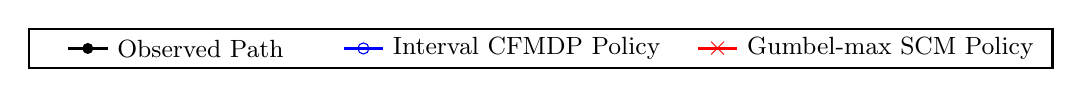
\begin{tikzpicture}[scale=1.0, every node/.style={scale=1.0}]
            \draw[thick, black] (-3, -0.25) rectangle (10, 0.25);
            %
            \draw[black, line width=1pt] (-2.5, 0.0) -- (-2,0.0);
            \fill[black] (-2.25,0.0) circle (2pt); %
            \node[right] at (-2,0.0) {\small Observed Path};
            
            %
            \draw[blue, line width=1pt] (1.0,0.0) -- (1.5,0.0);
            \node[draw=blue, circle, minimum size=4pt, inner sep=0pt] at (1.25,0.0) {}; %
            \node[right] at (1.5,0.0) {\small Interval CFMDP Policy};
            
            %
            \draw[red, line width=1pt] (5.5,0) -- (6,0);
            \node[red] at (5.75,0) {$\boldsymbol{\times}$}; %
            \node[right] at (6,0) {\small Gumbel-max SCM Policy};
        \end{tikzpicture}
    }\\
    %
    \subfigure[\footnotesize Lowest cumulative reward: Interval CFMDP ($312$), Gumbel-max SCM ($312$)]{%
        \resizebox{0.76\columnwidth}{!}{
             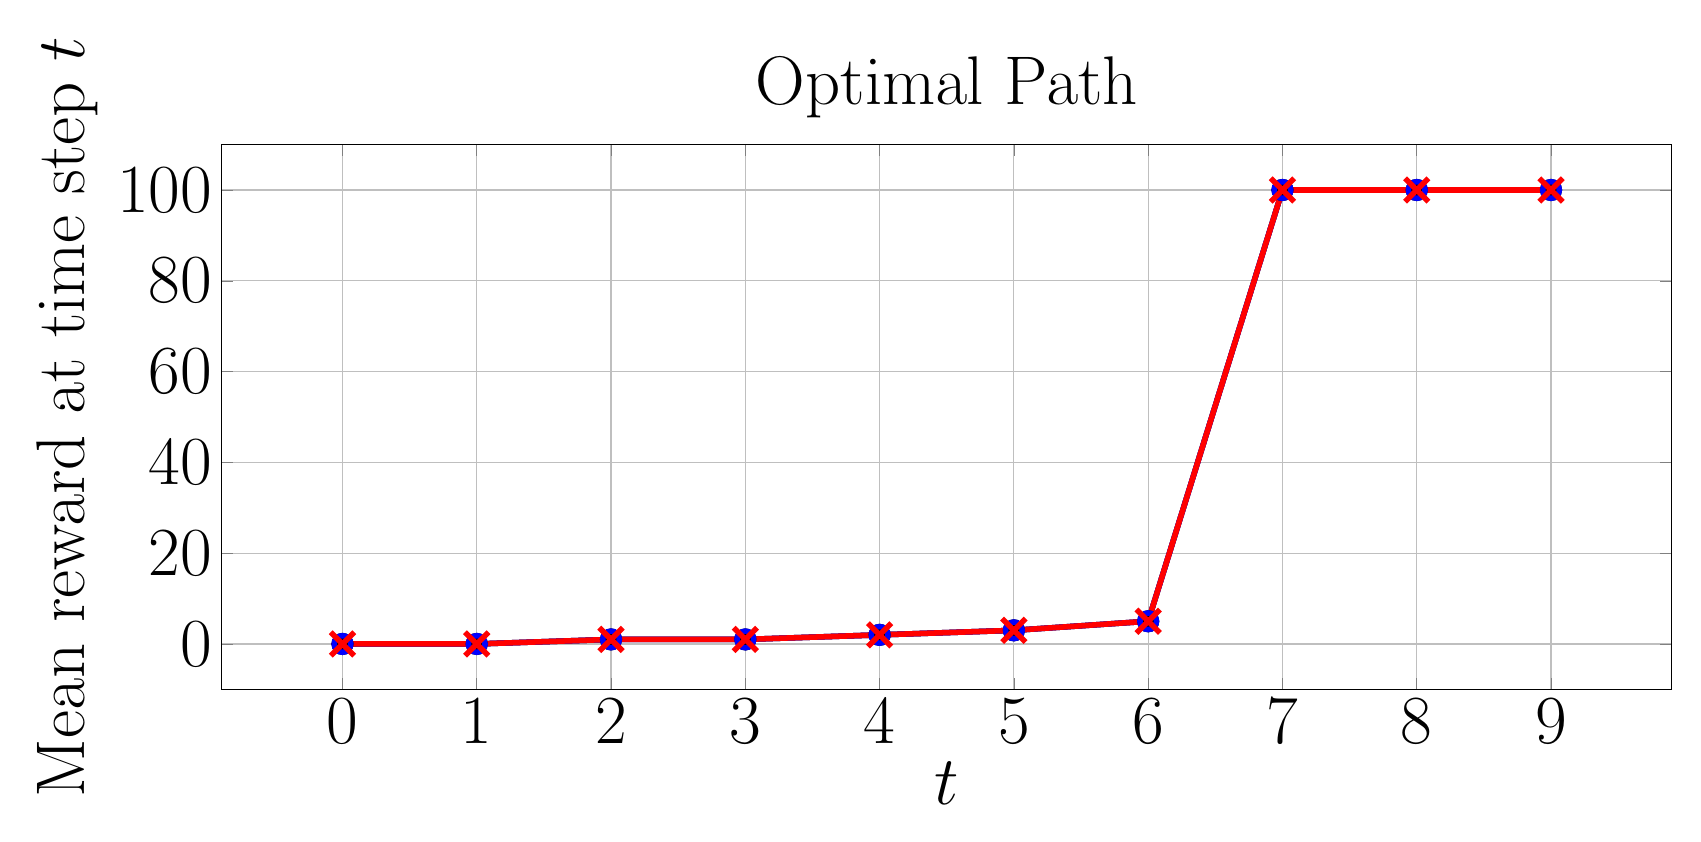
\begin{tikzpicture}
                \begin{axis}[
                    xlabel={$t$},
                    ylabel={Mean reward at time step $t$},
                    title={Optimal Path},
                    grid=both,
                    width=20cm, height=8.5cm,
                    every axis/.style={font=\Huge},
                    %
                ]
                \addplot[
                    color=black, %
                    mark=*, %
                    line width=2pt,
                    mark size=3pt,
                    error bars/.cd,
                    y dir=both, %
                    y explicit, %
                    error bar style={line width=1pt,solid},
                    error mark options={line width=1pt,mark size=4pt,rotate=90}
                ]
                coordinates {
                    (0, 0.0)  +- (0, 0.0)
                    (1, 0.0)  +- (0, 0.0) 
                    (2, 1.0)  +- (0, 0.0) 
                    (3, 1.0)  +- (0, 0.0)
                    (4, 2.0)  +- (0, 0.0)
                    (5, 3.0) +- (0, 0.0)
                    (6, 5.0) +- (0, 0.0)
                    (7, 100.0) +- (0, 0.0)
                    (8, 100.0) +- (0, 0.0)
                    (9, 100.0) +- (0, 0.0)
                };
                %
                \addplot[
                    color=blue, %
                    mark=o, %
                    line width=2pt,
                    mark size=3pt,
                    error bars/.cd,
                    y dir=both, %
                    y explicit, %
                    error bar style={line width=1pt,solid},
                    error mark options={line width=1pt,mark size=4pt,rotate=90}
                ]
                 coordinates {
                    (0, 0.0)  +- (0, 0.0)
                    (1, 0.0)  +- (0, 0.0) 
                    (2, 1.0)  +- (0, 0.0) 
                    (3, 1.0)  +- (0, 0.0)
                    (4, 2.0)  +- (0, 0.0)
                    (5, 3.0) +- (0, 0.0)
                    (6, 5.0) +- (0, 0.0)
                    (7, 100.0) +- (0, 0.0)
                    (8, 100.0) +- (0, 0.0)
                    (9, 100.0) +- (0, 0.0)
                };
                %
                \addplot[
                    color=red, %
                    mark=x, %
                    line width=2pt,
                    mark size=6pt,
                    error bars/.cd,
                    y dir=both, %
                    y explicit, %
                    error bar style={line width=1pt,solid},
                    error mark options={line width=1pt,mark size=4pt,rotate=90}
                ]
                coordinates {
                    (0, 0.0)  +- (0, 0.0)
                    (1, 0.0)  +- (0, 0.0) 
                    (2, 1.0)  +- (0, 0.0) 
                    (3, 1.0)  +- (0, 0.0)
                    (4, 2.0)  +- (0, 0.0)
                    (5, 3.0) +- (0, 0.0)
                    (6, 5.0) +- (0, 0.0)
                    (7, 100.0) +- (0, 0.0)
                    (8, 100.0) +- (0, 0.0)
                    (9, 100.0) +- (0, 0.0)
                };
                \end{axis}
            \end{tikzpicture}
         }
    }
    \hspace{1cm}
    \subfigure[\footnotesize Lowest cumulative reward: Interval CFMDP ($19$), Gumbel-max SCM ($-88$)]{%
         \resizebox{0.76\columnwidth}{!}{
            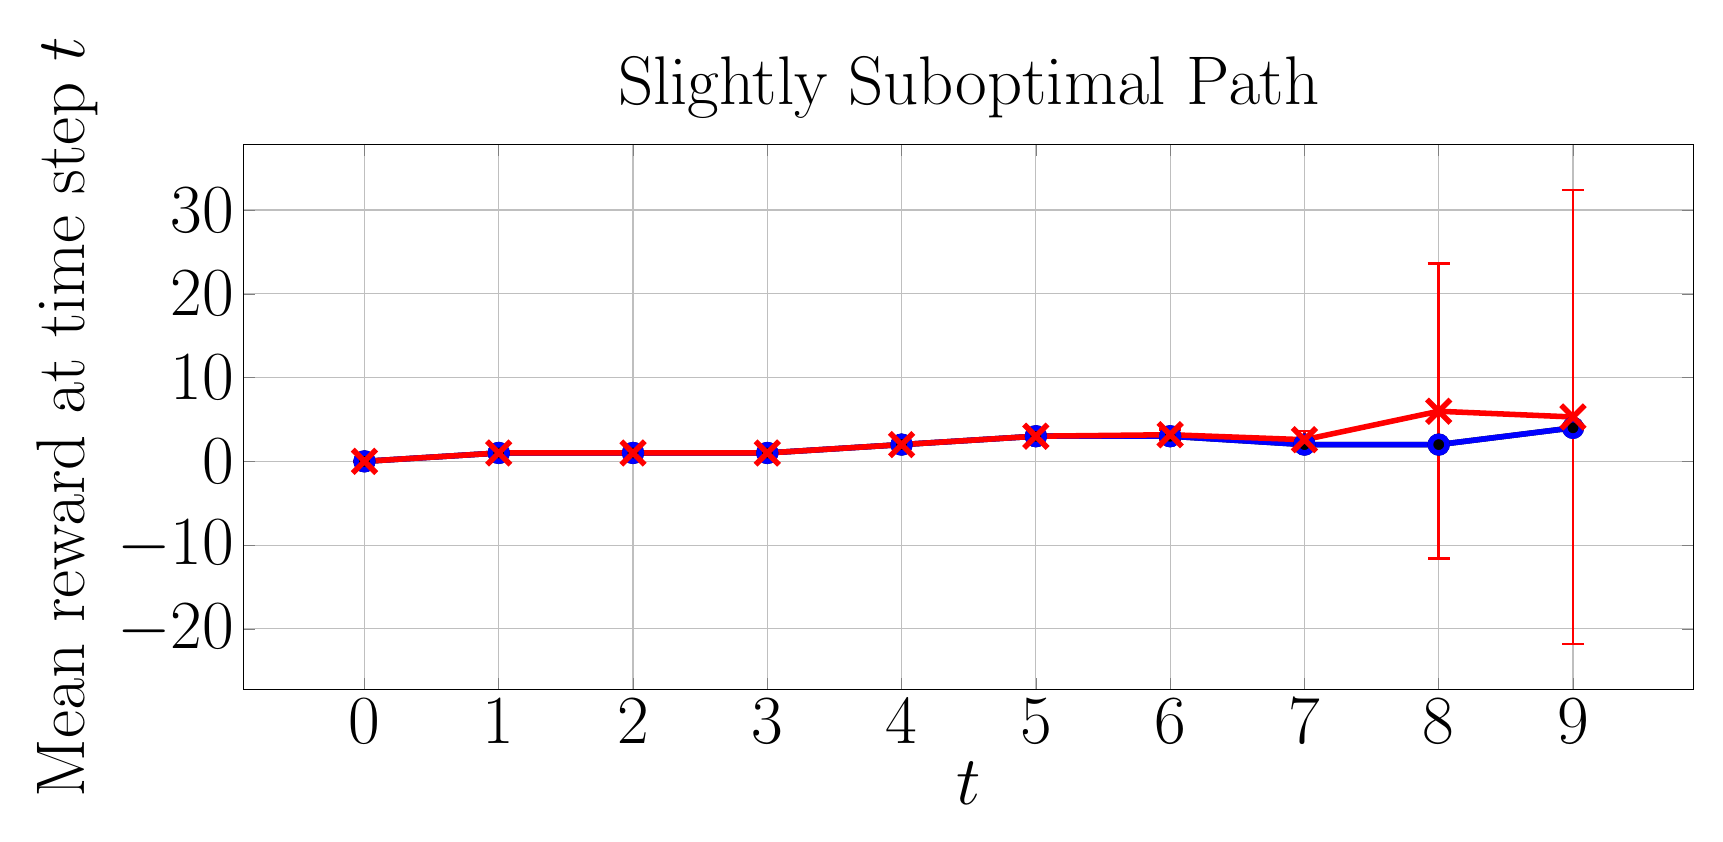
\begin{tikzpicture}
                \begin{axis}[
                    xlabel={$t$},
                    ylabel={Mean reward at time step $t$},
                    title={Slightly Suboptimal Path},
                    grid=both,
                    width=20cm, height=8.5cm,
                    every axis/.style={font=\Huge},
                    %
                ]
                \addplot[
                    color=black, %
                    mark=*, %
                    line width=2pt,
                    mark size=3pt,
                    error bars/.cd,
                    y dir=both, %
                    y explicit, %
                    error bar style={line width=1pt,solid},
                    error mark options={line width=1pt,mark size=4pt,rotate=90}
                ]
              coordinates {
                    (0, 0.0)  +- (0, 0.0)
                    (1, 1.0)  +- (0, 0.0) 
                    (2, 1.0)  +- (0, 0.0) 
                    (3, 1.0)  +- (0, 0.0)
                    (4, 2.0)  +- (0, 0.0)
                    (5, 3.0) +- (0, 0.0)
                    (6, 3.0) +- (0, 0.0)
                    (7, 2.0) +- (0, 0.0)
                    (8, 2.0) +- (0, 0.0)
                    (9, 4.0) +- (0, 0.0)
                };
                %
                \addplot[
                    color=blue, %
                    mark=o, %
                    line width=2pt,
                    mark size=3pt,
                    error bars/.cd,
                    y dir=both, %
                    y explicit, %
                    error bar style={line width=1pt,solid},
                    error mark options={line width=1pt,mark size=4pt,rotate=90}
                ]
              coordinates {
                    (0, 0.0)  +- (0, 0.0)
                    (1, 1.0)  +- (0, 0.0) 
                    (2, 1.0)  +- (0, 0.0) 
                    (3, 1.0)  +- (0, 0.0)
                    (4, 2.0)  +- (0, 0.0)
                    (5, 3.0) +- (0, 0.0)
                    (6, 3.0) +- (0, 0.0)
                    (7, 2.0) +- (0, 0.0)
                    (8, 2.0) +- (0, 0.0)
                    (9, 4.0) +- (0, 0.0)
                };
                %
                \addplot[
                    color=red, %
                    mark=x, %
                    line width=2pt,
                    mark size=6pt,
                    error bars/.cd,
                    y dir=both, %
                    y explicit, %
                    error bar style={line width=1pt,solid},
                    error mark options={line width=1pt,mark size=4pt,rotate=90}
                ]
                coordinates {
                    (0, 0.0)  +- (0, 0.0)
                    (1, 1.0)  +- (0, 0.0) 
                    (2, 1.0)  +- (0, 0.0) 
                    (3, 1.0)  +- (0, 0.0)
                    (4, 2.0)  += (0, 0.0)
                    (5, 3.0)  += (0, 0.0)
                    (6, 3.17847) += (0, 0.62606746) -= (0, 0.62606746)
                    (7, 2.5832885) += (0, 1.04598233) -= (0, 1.04598233)
                    (8, 5.978909) += (0, 17.60137623) -= (0, 17.60137623)
                    (9, 5.297059) += (0, 27.09227512) -= (0, 27.09227512)
                };
                \end{axis}
            \end{tikzpicture}
         }
    }\\[-1.5pt]
    \subfigure[\footnotesize Lowest cumulative reward: Interval CFMDP ($14$), Gumbel-max SCM ($-598$)]{%
         \resizebox{0.76\columnwidth}{!}{
             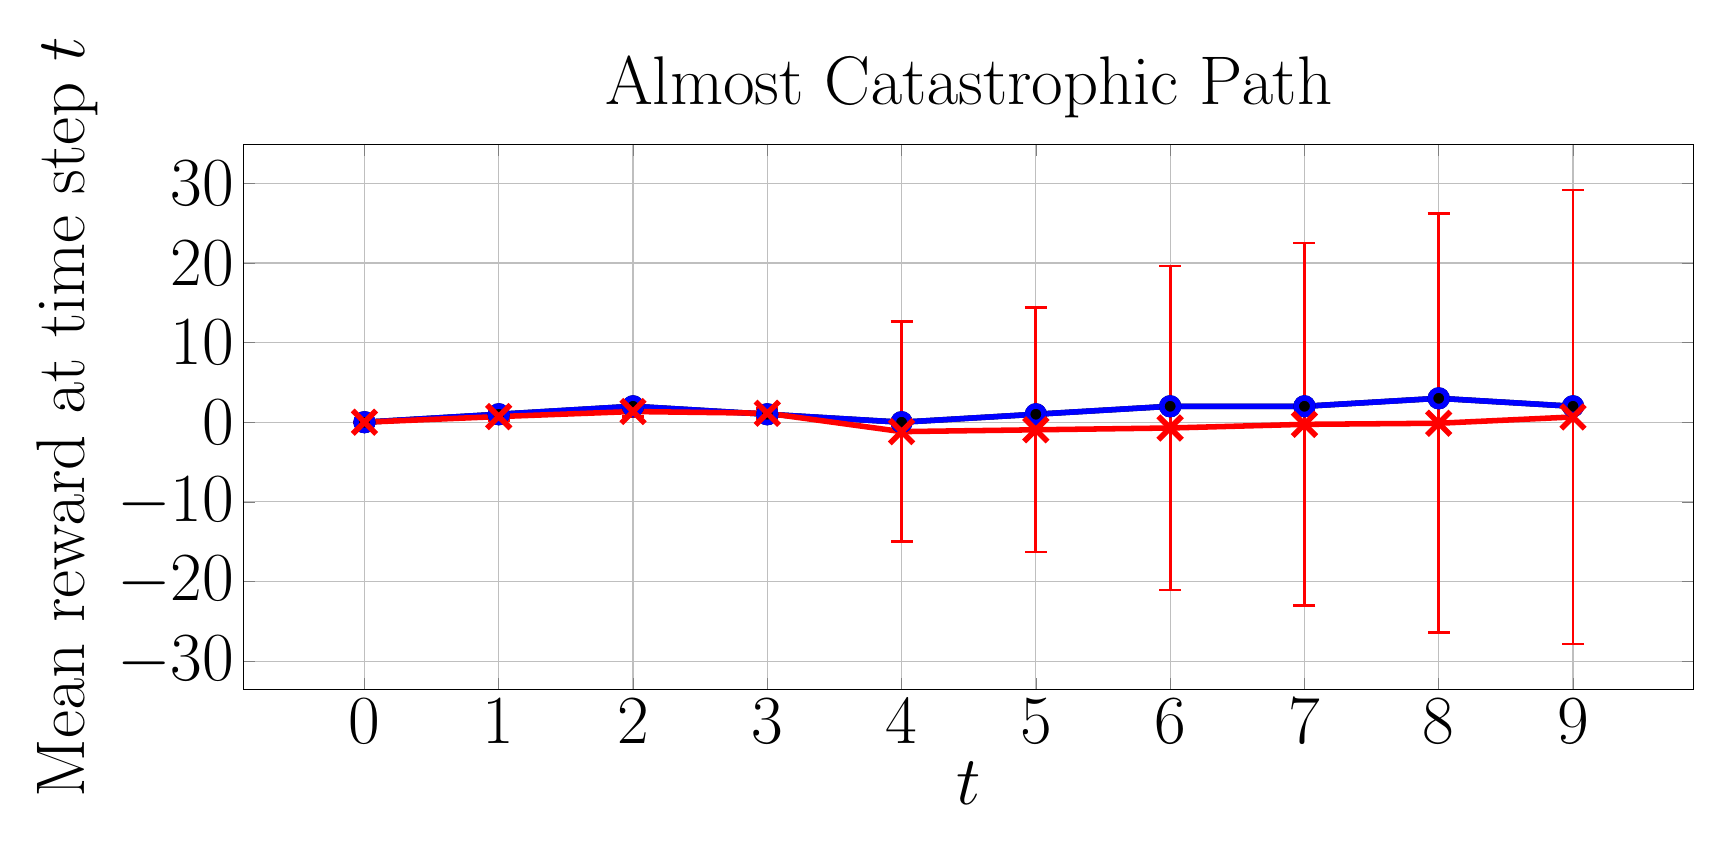
\begin{tikzpicture}
                \begin{axis}[
                    xlabel={$t$},
                    ylabel={Mean reward at time step $t$},
                    title={Almost Catastrophic Path},
                    grid=both,
                    width=20cm, height=8.5cm,
                    every axis/.style={font=\Huge},
                    %
                ]
                \addplot[
                    color=black, %
                    mark=*, %
                    line width=2pt,
                    mark size=3pt,
                    error bars/.cd,
                    y dir=both, %
                    y explicit, %
                    error bar style={line width=1pt,solid},
                    error mark options={line width=1pt,mark size=4pt,rotate=90}
                ]
                coordinates {
                    (0, 0.0)  +- (0, 0.0)
                    (1, 1.0)  +- (0, 0.0) 
                    (2, 2.0)  +- (0, 0.0) 
                    (3, 1.0)  +- (0, 0.0)
                    (4, 0.0)  +- (0, 0.0)
                    (5, 1.0) +- (0, 0.0)
                    (6, 2.0) +- (0, 0.0)
                    (7, 2.0) +- (0, 0.0)
                    (8, 3.0) +- (0, 0.0)
                    (9, 2.0) +- (0, 0.0)
                };
                %
                \addplot[
                    color=blue, %
                    mark=o, %
                    line width=2pt,
                    mark size=3pt,
                    error bars/.cd,
                    y dir=both, %
                    y explicit, %
                    error bar style={line width=1pt,solid},
                    error mark options={line width=1pt,mark size=4pt,rotate=90}
                ]
                coordinates {
                    (0, 0.0)  +- (0, 0.0)
                    (1, 1.0)  +- (0, 0.0) 
                    (2, 2.0)  +- (0, 0.0) 
                    (3, 1.0)  +- (0, 0.0)
                    (4, 0.0)  +- (0, 0.0)
                    (5, 1.0) +- (0, 0.0)
                    (6, 2.0) +- (0, 0.0)
                    (7, 2.0) +- (0, 0.0)
                    (8, 3.0) +- (0, 0.0)
                    (9, 2.0) +- (0, 0.0)
                };
                %
                \addplot[
                    color=red, %
                    mark=x, %
                    line width=2pt,
                    mark size=6pt,
                    error bars/.cd,
                    y dir=both, %
                    y explicit, %
                    error bar style={line width=1pt,solid},
                    error mark options={line width=1pt,mark size=4pt,rotate=90}
                ]
                coordinates {
                    (0, 0.0)  +- (0, 0.0)
                    (1, 0.7065655)  +- (0, 0.4553358) 
                    (2, 1.341673)  +- (0, 0.67091621) 
                    (3, 1.122926)  +- (0, 0.61281824)
                    (4, -1.1821935)  +- (0, 13.82444042)
                    (5, -0.952399)  +- (0, 15.35195457)
                    (6, -0.72672) +- (0, 20.33508414)
                    (7, -0.268983) +- (0, 22.77861454)
                    (8, -0.1310835) +- (0, 26.31013314)
                    (9, 0.65806) +- (0, 28.50670214)
                };
                %
            %
            %
            %
            %
            %
            %
            %
            %
            %
            %
            %
            %
            %
            %
            %
            %
            %
            %
                \end{axis}
            \end{tikzpicture}
         }
    }
    \hspace{1cm}
    \subfigure[\footnotesize Lowest cumulative reward: Interval CFMDP ($-698$), Gumbel-max SCM ($-698$)]{%
         \resizebox{0.76\columnwidth}{!}{
            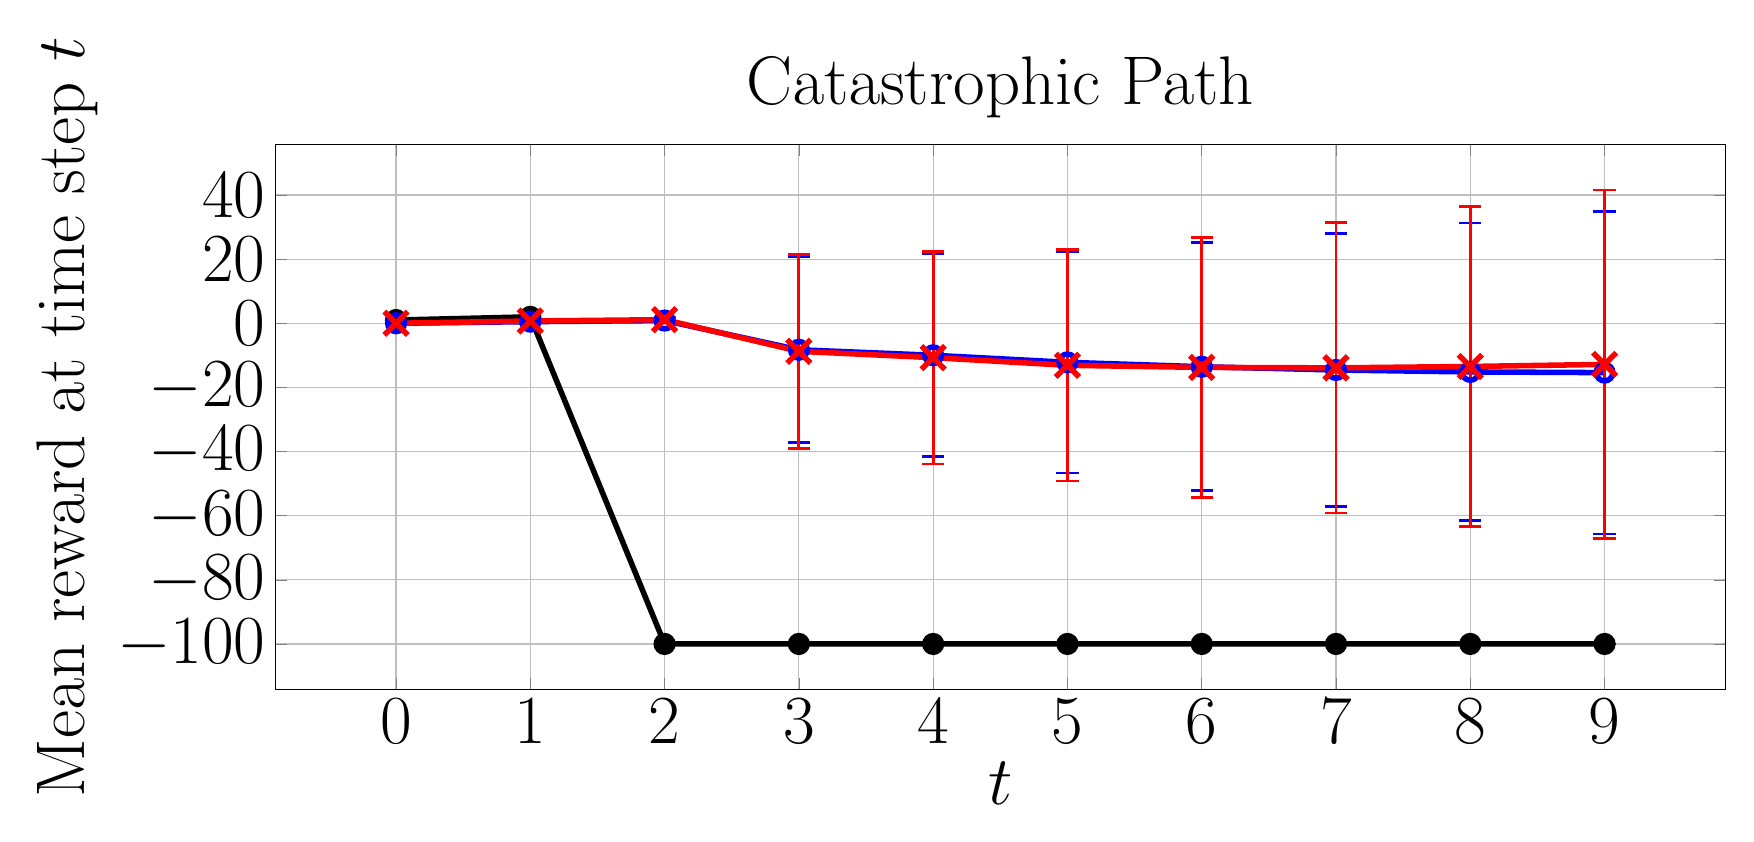
\begin{tikzpicture}
                \begin{axis}[
                    xlabel={$t$},
                    ylabel={Mean reward at time step $t$},
                    title={Catastrophic Path},
                    grid=both,
                    width=20cm, height=8.5cm,
                    every axis/.style={font=\Huge},
                    %
                ]
                \addplot[
                    color=black, %
                    mark=*, %
                    line width=2pt,
                    mark size=3pt,
                    error bars/.cd,
                    y dir=both, %
                    y explicit, %
                    error bar style={line width=1pt,solid},
                    error mark options={line width=1pt,mark size=4pt,rotate=90}
                ]
                coordinates {
                    (0, 1.0)  +- (0, 0.0)
                    (1, 2.0)  +- (0, 0.0) 
                    (2, -100.0)  +- (0, 0.0) 
                    (3, -100.0)  +- (0, 0.0)
                    (4, -100.0)  +- (0, 0.0)
                    (5, -100.0) +- (0, 0.0)
                    (6, -100.0) +- (0, 0.0)
                    (7, -100.0) +- (0, 0.0)
                    (8, -100.0) +- (0, 0.0)
                    (9, -100.0) +- (0, 0.0)
                };
                %
                \addplot[
                    color=blue, %
                    mark=o, %
                    line width=2pt,
                    mark size=3pt,
                    error bars/.cd,
                    y dir=both, %
                    y explicit, %
                    error bar style={line width=1pt,solid},
                    error mark options={line width=1pt,mark size=4pt,rotate=90}
                ]
                coordinates {
                    (0, 0.0)  +- (0, 0.0)
                    (1, 0.504814)  +- (0, 0.49997682) 
                    (2, 0.8439835)  +- (0, 0.76831917) 
                    (3, -8.2709165)  +- (0, 28.93656754)
                    (4, -9.981082)  +- (0, 31.66825363)
                    (5, -12.1776325) +- (0, 34.53463233)
                    (6, -13.556076) +- (0, 38.62845372)
                    (7, -14.574418) +- (0, 42.49603359)
                    (8, -15.1757075) +- (0, 46.41913968)
                    (9, -15.3900395) +- (0, 50.33563368)
                };
                %
                \addplot[
                    color=red, %
                    mark=x, %
                    line width=2pt,
                    mark size=6pt,
                    error bars/.cd,
                    y dir=both, %
                    y explicit, %
                    error bar style={line width=1pt,solid},
                    error mark options={line width=1pt,mark size=4pt,rotate=90}
                ]
                coordinates {
                    (0, 0.0)  +- (0, 0.0)
                    (1, 0.701873)  +- (0, 0.45743556) 
                    (2, 1.1227805)  +- (0, 0.73433129) 
                    (3, -8.7503255)  +- (0, 30.30257976)
                    (4, -10.722092)  +- (0, 33.17618589)
                    (5, -13.10721)  +- (0, 36.0648089)
                    (6, -13.7631645) +- (0, 40.56553451)
                    (7, -13.909043) +- (0, 45.23829402)
                    (8, -13.472517) +- (0, 49.96270296)
                    (9, -12.8278835) +- (0, 54.38618735)
                };
                %
            %
            %
            %
            %
            %
            %
            %
            %
            %
            %
            %
            %
            %
            %
            %
            %
            %
            %
                \end{axis}
            \end{tikzpicture}
         }
    }
    \caption{Average instant reward of CF paths induced by policies on GridWorld $p=0.4$.}
    \label{fig: reward p=0.4}
\end{figure*}

\subsection{Experimental Setup}
To compare policy performance, we measure the average rewards of counterfactual paths induced by our policy and the Gumbel-max policy by uniformly sampling $200$ counterfactual MDPs from the ICFMDP and generating $10,000$ counterfactual paths over each sampled CFMDP. \jl{Since the interval CFMDP depends on the observed path, we select $4$  paths of varying optimality to evaluate how the observed path impacts the performance of both policies: an optimal path, a slightly suboptimal path that could reach the optimal reward with a few changes, a catastrophic path that enters a catastrophic, terminal state with low reward, and an almost catastrophic path that was close to entering a catastrophic state.} When measuring the average probability bound widths and execution time needed to generate the ICFMDPs, we averaged over $20$ randomly generated observed paths
\footnote{Further training details are provided in Appendix \ref{app: training details}, and the code is provided at \href{https://github.com/ddv-lab/robust-cf-inference-in-MDPs}{https://github.com/ddv-lab/robust-cf-inference-in-MDPs}
%
%
.}.

\subsection{GridWorld}
\jl{The GridWorld MDP is a $4 \times 4$ grid where an agent must navigate from the top-left corner to the goal state in the bottom-right corner, avoiding a dangerous terminal state in the centre. At each time step, the agent can move up, down, left, or right, but there is a small probability (controlled by hyper-parameter $p$) of moving in an unintended direction. As the agent nears the goal, the reward for each state increases, culminating in a reward of $+100$ for reaching the goal. Entering the dangerous state results in a penalty of $-100$. We use two versions of GridWorld: a less stochastic version with $p=0.9$ (i.e., $90$\% chance of moving in the chosen direction) and a more stochastic version with $p=0.4$.}

\paragraph{GridWorld ($p=0.9$)}
When $p=0.9$, the counterfactual probability bounds are typically narrow (see Table \ref{tab:nonzero_probs} for average measurements). Consequently, as shown in Figure \ref{fig: reward p=0.9}, both policies are nearly identical and perform similarly well across the optimal, slightly suboptimal, and catastrophic paths.
%
However, for the almost catastrophic path, the interval CFMDP path is more conservative and follows the observed path more closely (as this is where the probability bounds are narrowest), which typically requires one additional step to reach the goal state than the Gumbel-max SCM policy.
%

\paragraph{GridWorld ($p=0.4$)}
\jl{When $p=0.4$, the GridWorld environment becomes more uncertain, increasing the risk of entering the dangerous state even if correct actions are chosen. Thus, as shown in Figure \ref{fig: reward p=0.4}, the interval CFMDP policy adopts a more conservative approach, avoiding deviation from the observed policy if it cannot guarantee higher counterfactual rewards (see the slightly suboptimal and almost catastrophic paths), whereas the Gumbel-max SCM is inconsistent: it can yield higher rewards, but also much lower rewards, reflected in the wide error bars.} For the catastrophic path, both policies must deviate from the observed path to achieve a higher reward and, in this case, perform similarly.
%
%
%
%
\subsection{Sepsis}
The Sepsis MDP \citep{oberst2019counterfactual} simulates trajectories of Sepsis patients. Each state consists of four vital signs (heart rate, blood pressure, oxygen concentration, and glucose levels), categorised as low, normal, or high.
and three treatments that can be toggled on/off at each time step (8 actions in total). Unlike \citet{oberst2019counterfactual}, we scale rewards based on the number of out-of-range vital signs, between $-1000$ (patient dies) and $1000$ (patient discharged). \jl{Like the GridWorld $p=0.4$ experiment, the Sepsis MDP is highly uncertain, as many states are equally likely to lead to optimal and poor outcomes. Thus, as shown in Figure \ref{fig: reward sepsis}, both policies follow the observed optimal and almost catastrophic paths to guarantee rewards are no worse than the observation.} However, improving the catastrophic path requires deviating from the observation. Here, the Gumbel-max SCM policy, on average, performs better than the interval CFMDP policy. But, since both policies have lower bounds clipped at $-1000$, neither policy reliably improves over the observation. In contrast, for the slightly suboptimal path, the interval CFMDP policy performs significantly better, shown by its higher lower bounds. 
Moreover, in these two cases, the worst-case counterfactual path generated by the interval CFMDP policy is better than that of the Gumbel-max SCM policy,
indicating its greater robustness.
%
\begin{figure*}
    \centering
     \resizebox{0.6\textwidth}{!}{
        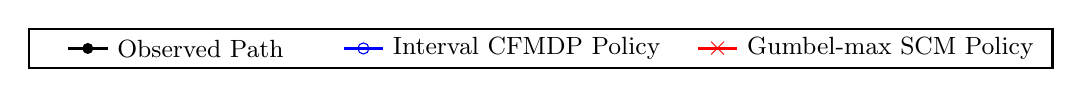
\begin{tikzpicture}[scale=1.0, every node/.style={scale=1.0}]
            \draw[thick, black] (-3, -0.25) rectangle (10, 0.25);
            %
            \draw[black, line width=1pt] (-2.5, 0.0) -- (-2,0.0);
            \fill[black] (-2.25,0.0) circle (2pt); %
            \node[right] at (-2,0.0) {\small Observed Path};
            
            %
            \draw[blue, line width=1pt] (1.0,0.0) -- (1.5,0.0);
            \node[draw=blue, circle, minimum size=4pt, inner sep=0pt] at (1.25,0.0) {}; %
            \node[right] at (1.5,0.0) {\small Interval CFMDP Policy};
            
            %
            \draw[red, line width=1pt] (5.5,0) -- (6,0);
            \node[red] at (5.75,0) {$\boldsymbol{\times}$}; %
            \node[right] at (6,0) {\small Gumbel-max SCM Policy};
        \end{tikzpicture}
    }\\
    \subfigure[\footnotesize Lowest cumulative reward: Interval CFMDP ($8000$), Gumbel-max SCM ($8000$)]{%
         \resizebox{0.76\columnwidth}{!}{
             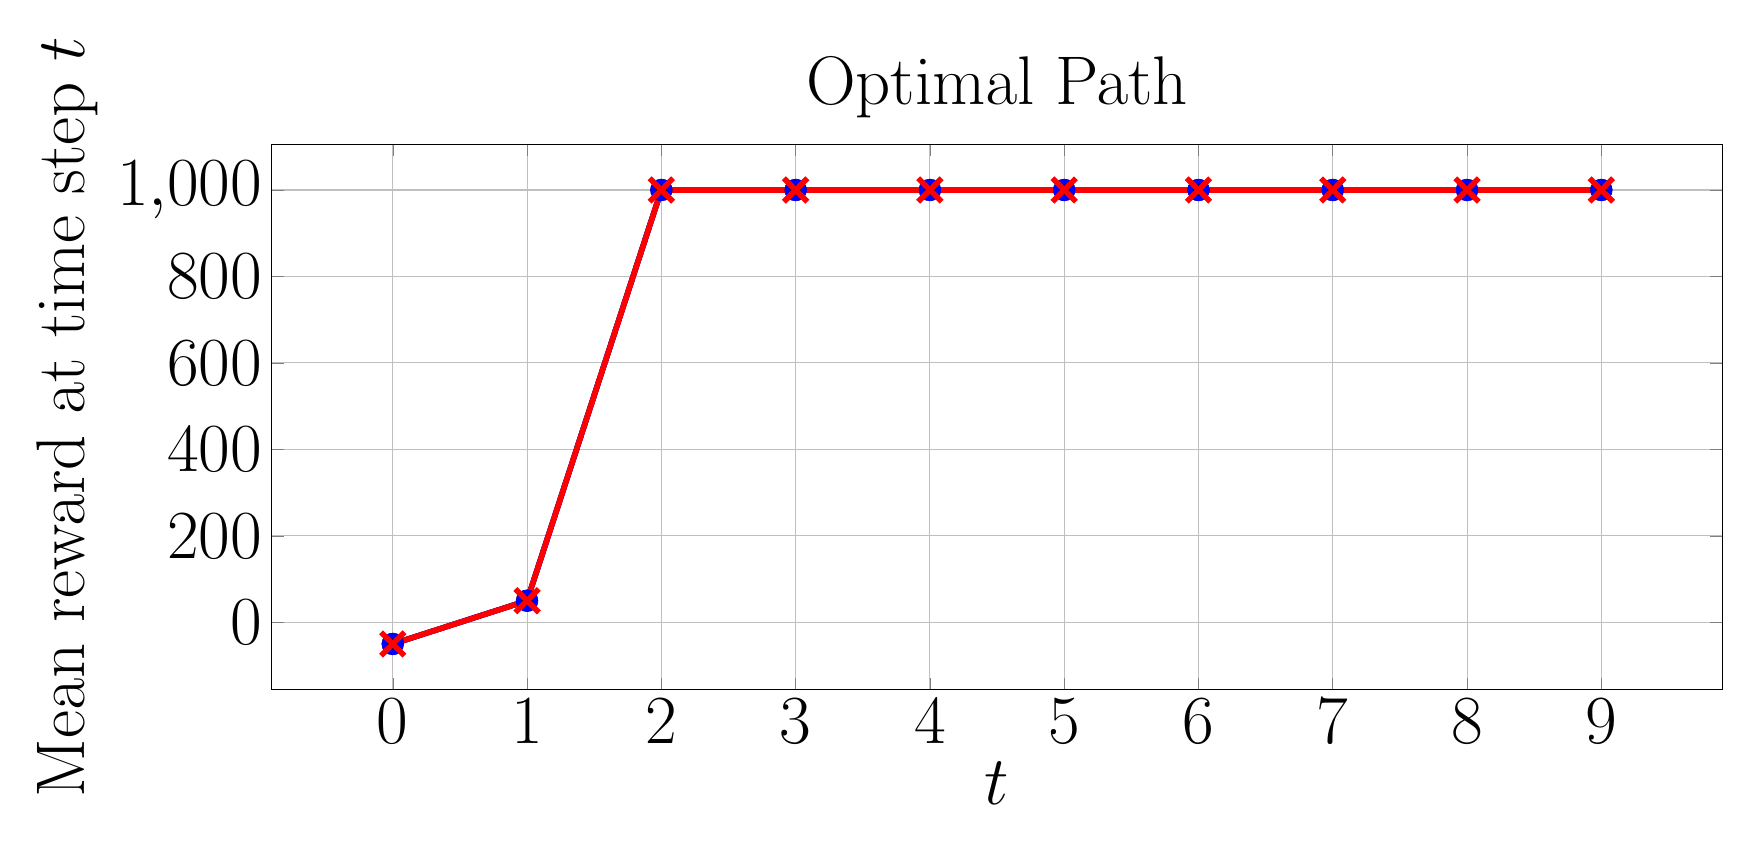
\begin{tikzpicture}
                \begin{axis}[
                    xlabel={$t$},
                    ylabel={Mean reward at time step $t$},
                    title={Optimal Path},
                    grid=both,
                    width=20cm, height=8.5cm,
                    every axis/.style={font=\Huge},
                    %
                ]
                \addplot[
                    color=black, %
                    mark=*, %
                    line width=2pt,
                    mark size=3pt,
                ]
                coordinates {
                    (0, -50.0)
                    (1, 50.0)
                    (2, 1000.0)
                    (3, 1000.0)
                    (4, 1000.0)
                    (5, 1000.0)
                    (6, 1000.0)
                    (7, 1000.0)
                    (8, 1000.0)
                    (9, 1000.0)
                };
                %
                \addplot[
                    color=blue, %
                    mark=o, %
                    line width=2pt,
                    mark size=3pt,
                    error bars/.cd,
                    y dir=both, %
                    y explicit, %
                    error bar style={line width=1pt,solid},
                    error mark options={line width=1pt,mark size=4pt,rotate=90}
                ]
                coordinates {
                    (0, -50.0)  +- (0, 0.0)
                    (1, 50.0)  +- (0, 0.0) 
                    (2, 1000.0)  +- (0, 0.0) 
                    (3, 1000.0)  +- (0, 0.0)
                    (4, 1000.0)  +- (0, 0.0)
                    (5, 1000.0) +- (0, 0.0)
                    (6, 1000.0) +- (0, 0.0)
                    (7, 1000.0) +- (0, 0.0)
                    (8, 1000.0) +- (0, 0.0)
                    (9, 1000.0) +- (0, 0.0)
                };
                %
                \addplot[
                    color=red, %
                    mark=x, %
                    line width=2pt,
                    mark size=6pt,
                    error bars/.cd,
                    y dir=both, %
                    y explicit, %
                    error bar style={line width=1pt,solid},
                    error mark options={line width=1pt,mark size=4pt,rotate=90}
                ]
                coordinates {
                    (0, -50.0)  +- (0, 0.0)
                    (1, 50.0)  +- (0, 0.0) 
                    (2, 1000.0)  +- (0, 0.0) 
                    (3, 1000.0)  +- (0, 0.0)
                    (4, 1000.0)  +- (0, 0.0)
                    (5, 1000.0) +- (0, 0.0)
                    (6, 1000.0) +- (0, 0.0)
                    (7, 1000.0) +- (0, 0.0)
                    (8, 1000.0) +- (0, 0.0)
                    (9, 1000.0) +- (0, 0.0)
                };
                %
                \end{axis}
            \end{tikzpicture}
         }
    }
    \hspace{1cm}
    \subfigure[\footnotesize Lowest cumulative reward: Interval CFMDP ($-5980$), Gumbel-max SCM ($-8000$)]{%
         \resizebox{0.76\columnwidth}{!}{
            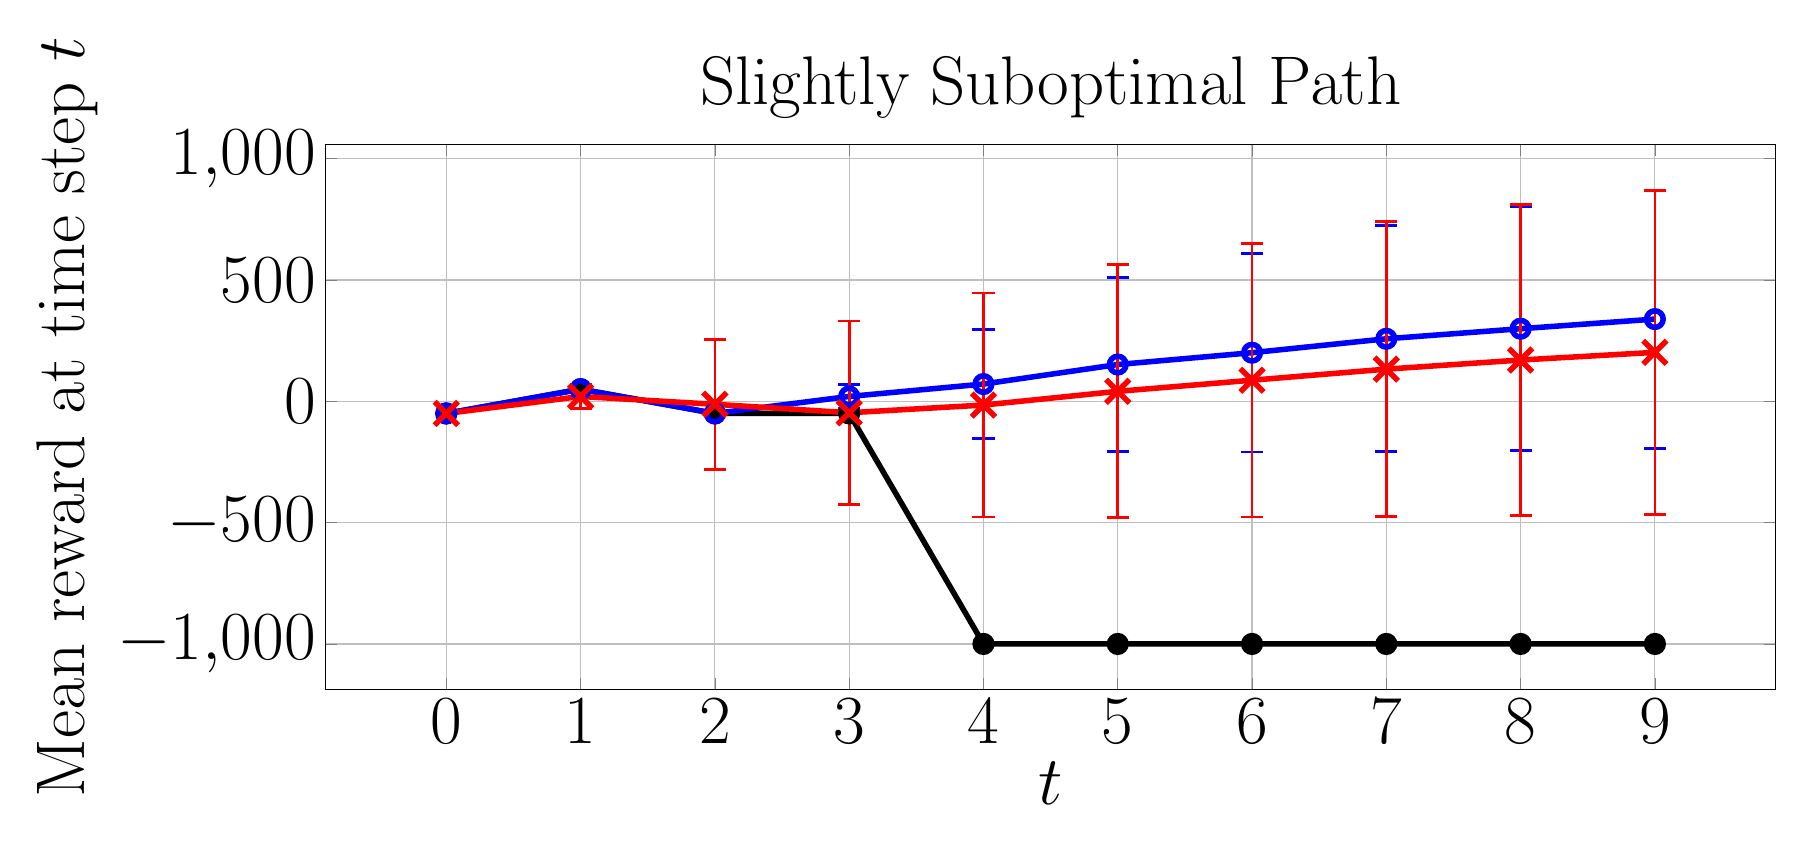
\begin{tikzpicture}
                \begin{axis}[
                    xlabel={$t$},
                    ylabel={Mean reward at time step $t$},
                    title={Slightly Suboptimal Path},
                    grid=both,
                    width=20cm, height=8.5cm,
                    every axis/.style={font=\Huge},
                    %
                ]
               \addplot[
                    color=black, %
                    mark=*, %
                    line width=2pt,
                    mark size=3pt,
                ]
                coordinates {
                    (0, -50.0)
                    (1, 50.0)
                    (2, -50.0)
                    (3, -50.0)
                    (4, -1000.0)
                    (5, -1000.0)
                    (6, -1000.0)
                    (7, -1000.0)
                    (8, -1000.0)
                    (9, -1000.0)
                };
                %
                \addplot[
                    color=blue, %
                    mark=o, %
                    line width=2pt,
                    mark size=3pt,
                    error bars/.cd,
                    y dir=both, %
                    y explicit, %
                    error bar style={line width=1pt,solid},
                    error mark options={line width=1pt,mark size=4pt,rotate=90}
                ]
                coordinates {
                    (0, -50.0)  +- (0, 0.0)
                    (1, 50.0)  +- (0, 0.0) 
                    (2, -50.0)  +- (0, 0.0) 
                    (3, 20.0631)  +- (0, 49.97539413)
                    (4, 71.206585)  +- (0, 226.02033693)
                    (5, 151.60797) +- (0, 359.23292559)
                    (6, 200.40593) +- (0, 408.86185176)
                    (7, 257.77948) +- (0, 466.10372804)
                    (8, 299.237465) +- (0, 501.82579506)
                    (9, 338.9129) +- (0, 532.06124996)
                };
                %
                \addplot[
                    color=red, %
                    mark=x, %
                    line width=2pt,
                    mark size=6pt,
                    error bars/.cd,
                    y dir=both, %
                    y explicit, %
                    error bar style={line width=1pt,solid},
                    error mark options={line width=1pt,mark size=4pt,rotate=90}
                ]
                coordinates {
                    (0, -50.0)  +- (0, 0.0)
                    (1, 20.00736)  +- (0, 49.99786741) 
                    (2, -12.282865)  +- (0, 267.598755) 
                    (3, -47.125995)  +- (0, 378.41755832)
                    (4, -15.381965)  +- (0, 461.77616558)
                    (5, 41.15459) +- (0, 521.53189262)
                    (6, 87.01595) +- (0, 564.22243126 )
                    (7, 132.62376) +- (0, 607.31338037)
                    (8, 170.168145) +- (0, 641.48013693)
                    (9, 201.813135) +- (0, 667.29441777)
                };
                %
                %
                %
                %
                %
                %
                %
                %
                %
                %
                %
                %
                %
                %
                %
                %
                %
                %
                %
                \end{axis}
            \end{tikzpicture}
         }
    }\\[-1.5pt]
    \subfigure[\footnotesize Lowest cumulative reward: Interval CFMDP ($100$), Gumbel-max SCM ($100$)]{%
         \resizebox{0.76\columnwidth}{!}{
             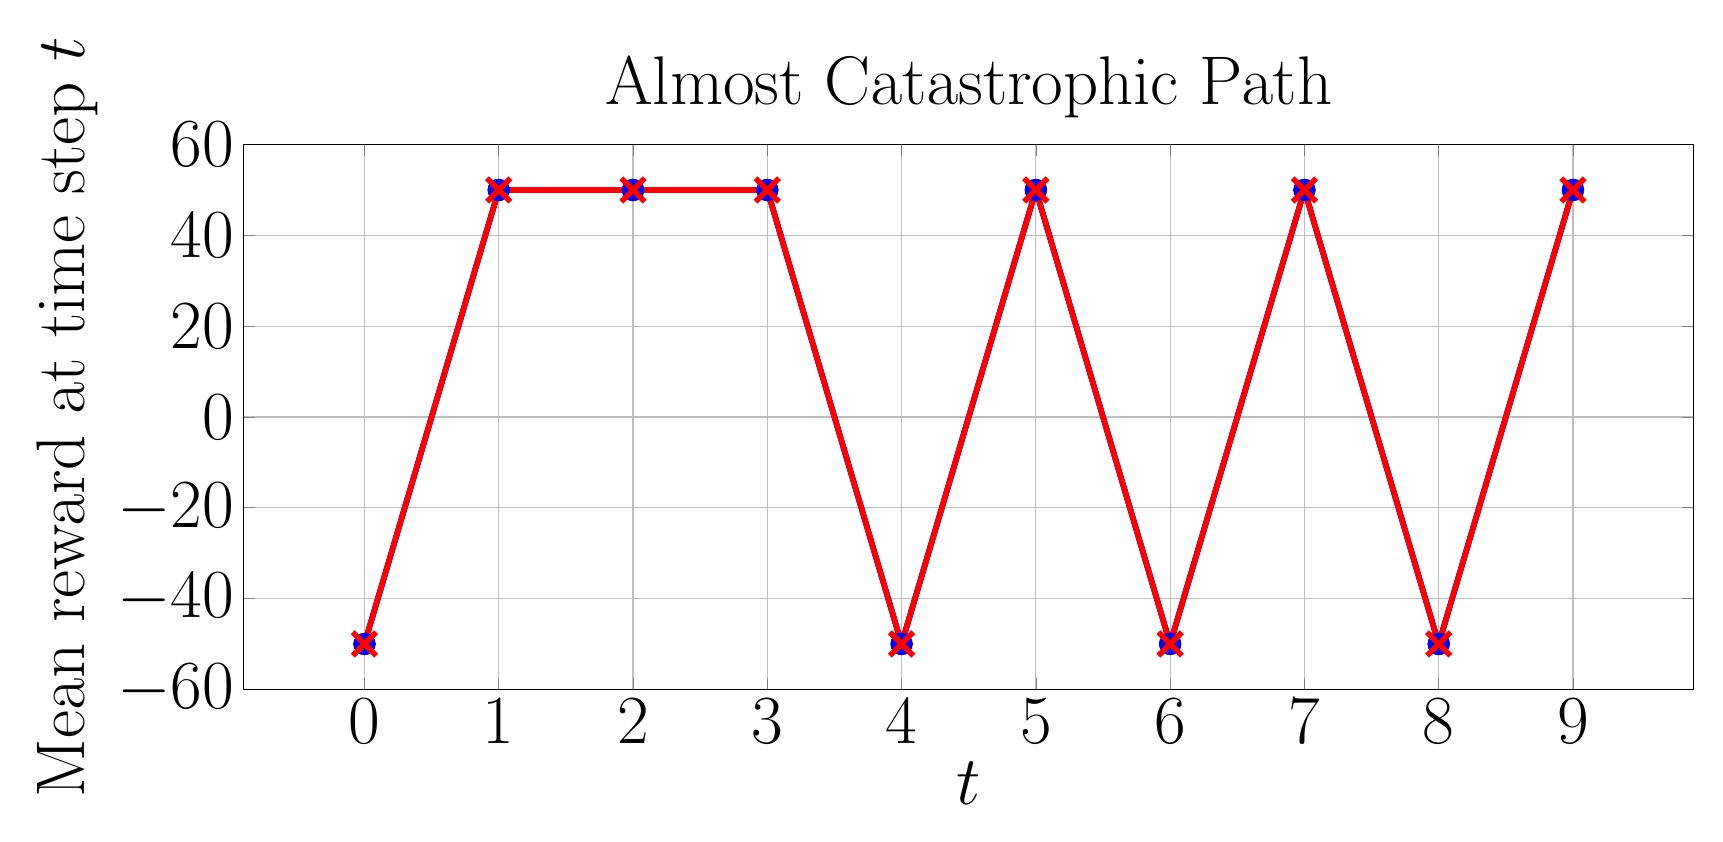
\begin{tikzpicture}
                \begin{axis}[
                    xlabel={$t$},
                    ylabel={Mean reward at time step $t$},
                    title={Almost Catastrophic Path},
                    grid=both,
                    every axis/.style={font=\Huge},
                    width=20cm, height=8.5cm,
                    %
                ]
               \addplot[
                    color=black, %
                    mark=*, %
                    line width=2pt,
                    mark size=3pt,
                ]
                coordinates {
                    (0, -50.0)
                    (1, 50.0)
                    (2, 50.0)
                    (3, 50.0)
                    (4, -50.0)
                    (5, 50.0)
                    (6, -50.0)
                    (7, 50.0)
                    (8, -50.0)
                    (9, 50.0)
                };
                %
                %
                \addplot[
                    color=blue, %
                    mark=o, %
                    line width=2pt,
                    mark size=3pt,
                    error bars/.cd,
                    y dir=both, %
                    y explicit, %
                    error bar style={line width=1pt,solid},
                    error mark options={line width=1pt,mark size=4pt,rotate=90}
                ]
                coordinates {
                    (0, -50.0)  +- (0, 0.0)
                    (1, 50.0)  +- (0, 0.0) 
                    (2, 50.0)  +- (0, 0.0) 
                    (3, 50.0)  +- (0, 0.0)
                    (4, -50.0)  +- (0, 0.0)
                    (5, 50.0) +- (0, 0.0)
                    (6, -50.0) +- (0, 0.0)
                    (7, 50.0) +- (0, 0.0)
                    (8, -50.0) +- (0, 0.0)
                    (9, 50.0) +- (0, 0.0)
                };
                %
                \addplot[
                    color=red, %
                    mark=x, %
                    line width=2pt,
                    mark size=6pt,
                    error bars/.cd,
                    y dir=both, %
                    y explicit, %
                    error bar style={line width=1pt,solid},
                    error mark options={line width=1pt,mark size=4pt,rotate=90}
                ]
                coordinates {
                    (0, -50.0)  +- (0, 0.0)
                    (1, 50.0)  +- (0, 0.0) 
                    (2, 50.0)  +- (0, 0.0) 
                    (3, 50.0)  +- (0, 0.0)
                    (4, -50.0)  +- (0, 0.0)
                    (5, 50.0) +- (0, 0.0)
                    (6, -50.0) +- (0, 0.0)
                    (7, 50.0) +- (0, 0.0)
                    (8, -50.0) +- (0, 0.0)
                    (9, 50.0) +- (0, 0.0)
                };
                %
                %
                %
                %
                %
                %
                %
                %
                %
                %
                %
                %
                %
                %
                %
                %
                %
                %
                %
                \end{axis}
            \end{tikzpicture}
         }
    }
    \hspace{1cm}
    \subfigure[\footnotesize Lowest cumulative reward: Interval CFMDP ($-7150$), Gumbel-max SCM ($-9050$)]{%
         \resizebox{0.76\columnwidth}{!}{
            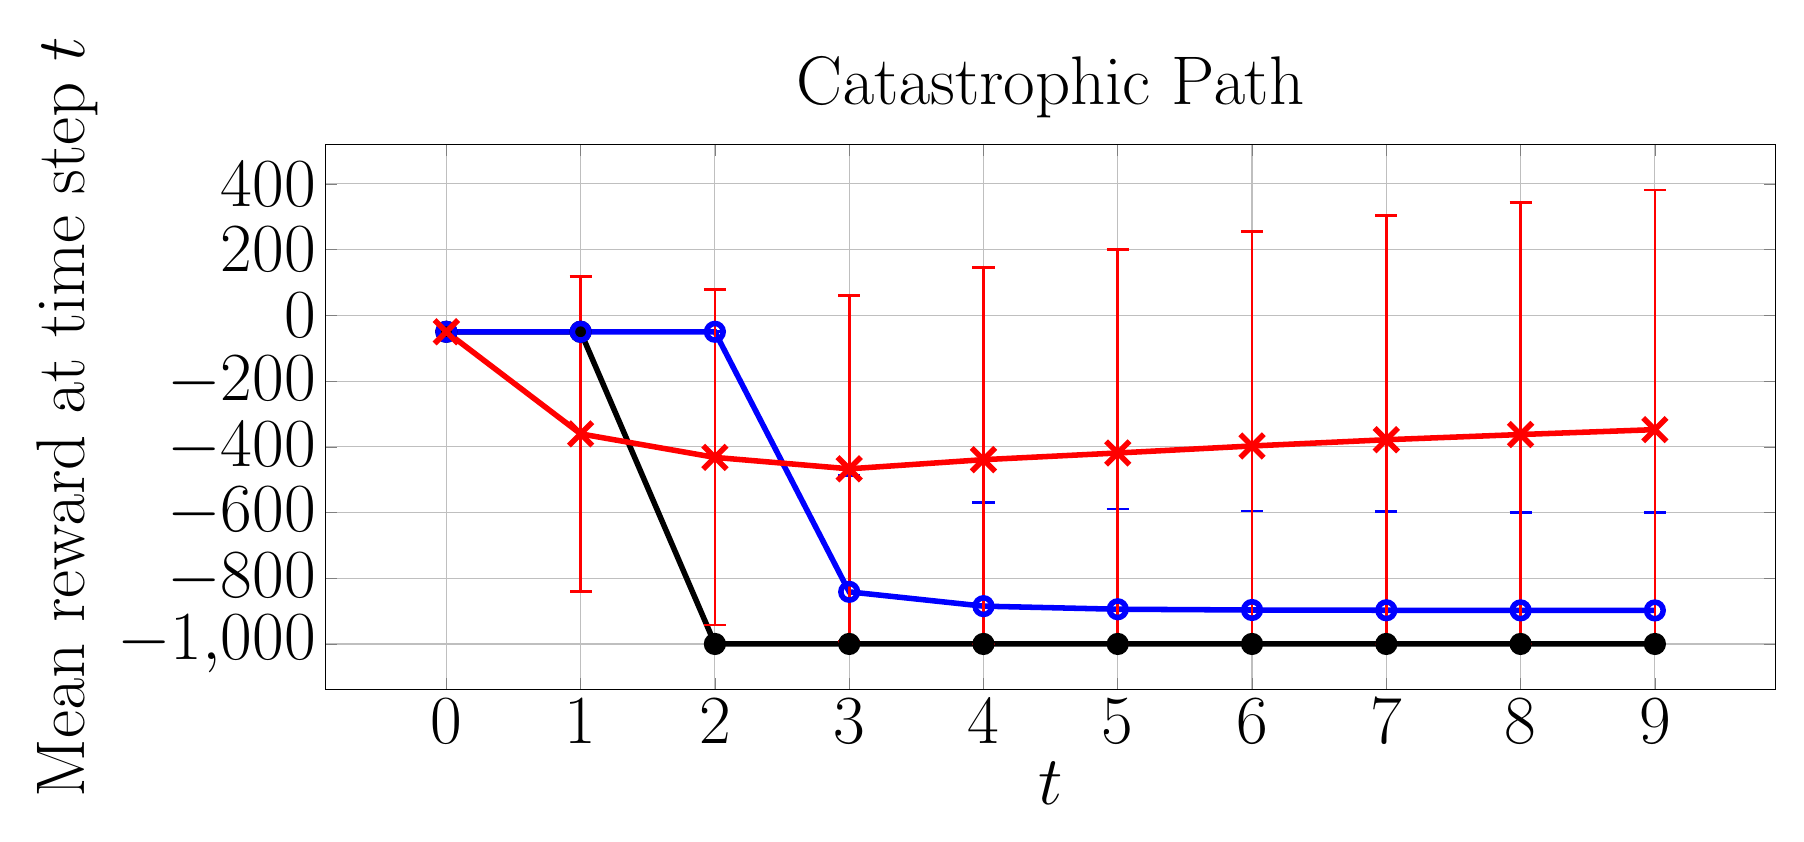
\begin{tikzpicture}
                \begin{axis}[
                    xlabel={$t$},
                    ylabel={Mean reward at time step $t$},
                    title={Catastrophic Path},
                    grid=both,
                    width=20cm, height=8.5cm,
                    every axis/.style={font=\Huge},
                    %
                ]
               \addplot[
                    color=black, %
                    mark=*, %
                    line width=2pt,
                    mark size=3pt,
                ]
                coordinates {
                    (0, -50.0)
                    (1, -50.0)
                    (2, -1000.0)
                    (3, -1000.0)
                    (4, -1000.0)
                    (5, -1000.0)
                    (6, -1000.0)
                    (7, -1000.0)
                    (8, -1000.0)
                    (9, -1000.0)
                };
                %
                %
                \addplot[
                    color=blue, %
                    mark=o, %
                    line width=2pt,
                    mark size=3pt,
                    error bars/.cd,
                    y dir=both, %
                    y explicit, %
                    error bar style={line width=1pt,solid},
                    error mark options={line width=1pt,mark size=4pt,rotate=90}
                ]
                coordinates {
                    (0, -50.0)  +- (0, 0.0)
                    (1, -50.0)  +- (0, 0.0) 
                    (2, -50.0)  +- (0, 0.0) 
                    (3, -841.440725)  += (0, 354.24605512) -= (0, 158.559275)
                    (4, -884.98225)  += (0, 315.37519669) -= (0, 115.01775)
                    (5, -894.330425) += (0, 304.88572805) -= (0, 105.669575)
                    (6, -896.696175) += (0, 301.19954514) -= (0, 103.303825)
                    (7, -897.4635) += (0, 299.61791279) -= (0, 102.5365)
                    (8, -897.77595) += (0, 298.80392585) -= (0, 102.22405)
                    (9, -897.942975) += (0, 298.32920557) -= (0, 102.057025)
                };
                %
                \addplot[
                    color=red, %
                    mark=x, %
                    line width=2pt,
                    mark size=6pt,
                    error bars/.cd,
                    y dir=both, %
                    y explicit, %
                    error bar style={line width=1pt,solid},
                    error mark options={line width=1pt,mark size=4pt,rotate=90}
                ]
            coordinates {
                    (0, -50.0)  +- (0, 0.0)
                    (1, -360.675265)  +- (0, 479.39812699) 
                    (2, -432.27629)  +- (0, 510.38620897) 
                    (3, -467.029545)  += (0, 526.36009628) -= (0, 526.36009628)
                    (4, -439.17429)  += (0, 583.96638919) -= (0, 560.82571)
                    (5, -418.82704) += (0, 618.43027478) -= (0, 581.17296)
                    (6, -397.464895) += (0, 652.67322574) -= (0, 602.535105)
                    (7, -378.49052) += (0, 682.85407033) -= (0, 621.50948)
                    (8, -362.654195) += (0, 707.01412023) -= (0, 637.345805)
                    (9, -347.737935) += (0, 729.29076479) -= (0, 652.262065)
                };
                %
                %
                %
                %
                %
                %
                %
                %
                %
                %
                %
                %
                %
                %
                %
                %
                %
                %
                %
                \end{axis}
            \end{tikzpicture}
         }
    }
    \caption{Average instant reward of CF paths induced by policies on Sepsis.}
    \label{fig: reward sepsis}
\end{figure*}

%
%
%
\subsection{Interval CFMDP Bounds}
%
%
Table \ref{tab:nonzero_probs} presents the mean counterfactual probability bound widths (excluding transitions where the upper bound is $0$) for each MDP, averaged over 20 observed paths. We compare the bounds under counterfactual stability (CS) and monotonicity (M) assumptions, CS alone, and no assumptions. This shows that the assumptions marginally reduce the bound widths, indicating the assumptions tighten the bounds without excluding too many causal models, as intended.
\renewcommand{\arraystretch}{1}

\begin{table}
\centering
\caption{Mean width of counterfactual probability bounds}
\resizebox{0.8\columnwidth}{!}{%
\begin{tabular}{|c|c|c|c|}
\hline
\multirow{2}{*}{\textbf{Environment}} & \multicolumn{3}{c|}{\textbf{Assumptions}} \\ \cline{2-4}
 & \textbf{CS + M} & \textbf{CS} & \textbf{None\tablefootnote{\jl{Equivalent to \citet{li2024probabilities}'s bounds (see Section \ref{sec: equivalence with Li}).}}} \\ \hline
\textbf{GridWorld} ($p=0.9$) & 0.0817 & 0.0977 & 0.100 \\ \hline
\textbf{GridWorld} ($p=0.4$) & 0.552  & 0.638  & 0.646 \\ \hline
\textbf{Sepsis} & 0.138 & 0.140 & 0.140 \\ \hline
\end{tabular}
}
\label{tab:nonzero_probs}
\end{table}


\subsection{Execution Times}
Table \ref{tab: times} compares the average time needed to generate the interval CFMDP vs.\ the Gumbel-max SCM CFMDP for 20 observations.
The GridWorld algorithms were run single-threaded, while the Sepsis experiments were run in parallel.
Generating the interval CFMDP is significantly faster as it uses exact analytical bounds, whereas the Gumbel-max CFMDP requires sampling from the Gumbel distribution to estimate counterfactual transition probabilities. \jl{Since constructing the counterfactual MDP models is the main bottleneck in both approaches, ours is more efficient overall and suitable for larger MDPs.}
\begin{table}
\centering
\caption{Mean execution time to generate CFMDPs}
\resizebox{0.99\columnwidth}{!}{%
\begin{tabular}{|c|c|c|}
\hline
\multirow{2}{*}{\textbf{Environment}} & \multicolumn{2}{c|}{\textbf{Mean Execution Time (s)}} \\ \cline{2-3} 
                                      & \textbf{Interval CFMDP} & \textbf{Gumbel-max CFMDP} \\ \hline
\textbf{GridWorld ($p=0.9$) }                  & 0.261                   & 56.1                      \\ \hline
\textbf{GridWorld ($p=0.4$)  }                 & 0.336                   & 54.5                      \\ \hline
\textbf{Sepsis}                                 & 688                     & 2940                      \\ \hline
\end{tabular}%
}
\label{tab: times}
\end{table}


\subsubsection{Results}
\section{Analysis}
\label{sec:analysis}
In the following sections, we will analyze European type approval regulation\footnote{Strictly speaking, the German enabling act (AFGBV) does not regulate type-approval, but how test \& operating permits are issued for SAE-Level-4 systems. Type-approval regulation for SAE-Level-3 systems follows UN Regulation No. 157 (UN-ECE-ALKS) \parencite{un157}.} regarding the underlying notions of ``safety'' and ``risk''.
We will classify these notions according to their absolute or relative character, underlying risk sources, or underlying concepts of harm.

\subsection{Classification of Safety Notions}
\label{sec:safety-notions}
We will refer to \emph{absolute} notions of safety as conceptualizations that assume the complete absence of any kind of risk.
Opposed to this, \emph{relative} notions of safety are based on a conceptualization that specifically includes risk acceptance criteria, e.g., in terms of ``tolerable'' risk or ``sufficient'' safety.

For classifying notions of safety by their underlying risk (or rather ``hazard'') sources, and different concepts of harm, \Cref{fig:hazard-sources} provides an overview of our reasoning, which is closely in line with the argumentation provided by Waymo in \parencite{favaro2023}.
We prefer ``hazard sources'' over ``risk sources'', as a risk must always be related to a \emph{cause} or \emph{source of harm} (i.e., a hazard \parencite[p.~1, def. 3.2]{iso51}).
Without a concrete (scenario) context that the system is operating in, a hazard is \emph{latent}: E.g., when operating in public traffic, there is a fundamental possibility that a \emph{collision with a pedestrian} leads to (physical) harm for that pedestrian. 
However, only if an automated vehicle shows (potentially) hazardous behavior (e.g., not decelerating properly) \emph{and} is located near a pedestrian (context), the hazard is instantiated and leads to a hazardous event.
\begin{figure*}
    \includeimg[width=.9\textwidth]{hazard-sources0.pdf}
    \caption{Graphical summary of a taxonomy of risk related to automated vehicles, extended based on ISO 21448 (\parencite{iso21448}) and \parencite{favaro2023}. Top: Causal chain from hazard sources to actual harm; bottom: summary of the individual elements' contributions to a resulting risk. Graphic translated from \parencite{nolte2024} \label{fig:hazard-sources}}
\end{figure*}
If the hazardous event cannot be mitigated or controlled, we see a loss event in which the pedestrian's health is harmed.
Note that this hypothetical chain of events is summarized in the definition of risk:
The probability of occurrence of harm is determined by a) the frequency with which hazard sources manifest, b) the time for which the system operates in a context that exposes the possibility of harm, and c) by the probability with which a hazardous event can be controlled.
A risk can then be determined as a function of the probability of harm and the severity of the harm potentially inflicted on the pedestrian.

In the following, we will apply this general model to introduce different types of hazard sources and also different types of harm.
\cref{fig:hazard-sources} shows two distinct hazard sources, i.e., functional insufficiencies and E/E-failures that can lead to hazardous behavior.
ISO~21488 \parencite{iso21448} defines functional insufficiencies as insufficiencies that stem from an incomplete or faulty system specification (specification insufficiencies).
In addition, the standard considers insufficiencies that stem from insufficient technical capability to operate inside the targeted Operational Design Domain (performance insufficiencies).
Functional insufficiencies are related to the ``Safety of the Intended Functionality (SOTIF)'' (according to ISO~21448), ``Behavioral Safety'' (according to Waymo \parencite{waymo2018}), or ``Operational Safety'' (according to UN Regulation No. 157 \parencite{un157}).
E/E-Failures are related to classic functional safety and are covered exhaustively by ISO~26262 \parencite{iso2018}.
Additional hazard sources can, e.g., be related to malicious security attacks (ISO~21434), or even to mechanical failures that should be covered (in the US) in the Federal Motor Vehicle Safety Standards (FMVSS).

For the classification of notions of safety by the related harm, in \parencite{salem2024, nolte2024}, we take a different approach compared to \parencite{koopman2024}:
We extend the concept of harm to the violation of stakeholder \emph{values}, where values are considered to be a ``standard of varying importance among other such standards that, when combined, form a value pattern that reduces complexity for stakeholders [\ldots] [and] determines situational actions [\ldots].'' \parencite{albert2008}
In this sense, values are profound, personal determinants for individual or collective behavior.
The notion of values being organized in a weighted value pattern shows that values can be ranked according to importance.
For automated vehicles, \emph{physical wellbeing} and \emph{mobility} can, e.g., be considered values which need to be balanced to achieve societal acceptance, in line with the discussion of required tradeoffs in \cref{sec:terminology}.
For the analysis of the following regulatory frameworks, we will evaluate if the given safety or risk notions allow tradeoffs regarding underlying stakeholder values. 

\subsection{UN Regulation No. 157 \& European Implementing Regulation (EU) 2022/1426}
\label{sec:enabling-act}
UN Regulation No. 157 \parencite{un157} and the European Implementing Regulation 2022/1426 \parencite{eu1426} provide type approval regulation for automated vehicles equipped with SAE-Level-3 (UN Reg. 157) and Level 4 (EU 2022/1426) systems on an international (UN Reg. 157) and European (EU 2022/1426) level.

Generally, EU type approval considers UN ECE regulations mandatory for its member states ((EU) 2018/858, \parencite{eu858}), while the EU largely forgoes implementing EU-specific type approval rules, it maintains the right to alter or to amend UN ECE regulation \parencite{eu858}.

In this respect, the terminology and conceptualizations in the EU Implementing Act closely follow those in UN Reg. No. 157.
The EU Implementing Act gives a clear reference to UN Reg. No. 157 \parencite[][Preamble,  Paragraph 1]{eu1426}.
Hence, the documents can be assessed in parallel.
Differences will be pointed out as necessary.

Both acts are written in rather technical language, including the formulation of technical requirements (e.g., regarding deceleration values or speeds in certain scenarios).
While providing exhaustive definitions and terminology, neither of both documents provide an actual definition of risk or safety.
The definition of ``unreasonable'' risk in both documents does not define risk, but only what is considered \emph{unreasonable}. It states that the ``overall level of risk for [the driver, (only in UN Reg. 157)] vehicle occupants and other road users which is increased compared to a competently and carefully driven manual vehicle.''
The pertaining notions of safety and risk can hence only be derived from the context in which they are used.

\subsubsection{Absolute vs. Relative Notions of Safety}
In line with the technical detail provided in the acts, both clearly imply a \emph{relative} notion of safety and refer to the absence of \emph{unreasonable} risk throughout, which is typical for technical safety definitions.

Both acts require sufficient proof and documentation that the to-be-approved automated driving systems are ``free of unreasonable safety risks to vehicle occupants and other road users'' for type approval.\footnote{As it targets SAE-Level-3 systems, UN Reg. 157 also refers to the driver, where applicable.}
In this respect, both acts demand that the manufacturers perform verification and validation activities for performance requirements that include ``[\ldots] the conclusion that the system is designed in such a way that it is free from unreasonable risks [\ldots]''.
Additionally, \emph{risk minimization} is a recurring theme when it comes to the definition of Minimum Risk Maneuvers (MRM).

Finally, supporting the relative notions of safety and risk, UN Reg. 157 introduces the concept of ``reasonable foreseeable and preventable'' \parencite[Article 1, Clause 5.1.1.]{un157} collisions, which implies that a residual risk will remain with the introduction of automated vehicles.
\parencite[][Appendix 3, Clause 3.1.]{un157} explicitly states that only \emph{some} scenarios that are unpreventable for a competent human driver can actually be prevented by an automated driving system.
While this concept is not applied throughout the EU Implementing Act, both documents explicitly refer to \emph{residual} risks that are related to the operation of automated driving systems (\parencite[][Annex I, Clause 1]{un157}, \parencite[][Annex II, Clause 7.1.1.]{eu1426}).

\subsubsection{Hazard Sources}
Hazard sources that are explicitly differentiated in UN Reg. 157 and (EU) 2022/1426 are E/E-failures that are in scope of functional safety (ISO~26262) and functional insufficiencies that are in scope of behavioral (or ``operational'') safety (ISO~21448).
Both documents consistently differentiate both sources when formulating requirements.

While the acts share a common definition of ``operational'' safety (\parencite[][Article 2, def. 30.]{eu1426}, \parencite[][Annex 4, def. 2.15.]{un157}), the definitions for functional safety differ.
\parencite{un157} defines functional safety as the ``absence of unreasonable risk under the occurrence of hazards caused by a malfunctioning behaviour of electric/electronic systems [\ldots]'', \parencite{eu1426} drops the specification of ``electric/electronic systems'' from the definition.
When taken at face value, this definition would mean that functional safety included all possible hazard sources, regardless of their origin, which is a deviation from the otherwise precise usage of safety-related terminology.

\subsubsection{Harm Types}
As the acts lack explicit definitions of safety and risk, there is no consistent and explicit notion of different harm types that could be differentiated.

\parencite{un157} gives little hints regarding different considered harm types.
``The absence of unreasonable risk'' in terms of human driving performance could hence be related to any chosen performance metric that allows a comparison with a competent careful human driver including, e.g., accident statistics, statistics about rule violations, or changes in traffic flow.

In \parencite{eu1426}, ``safety'' is, implicitly, attributed to the absence of unreasonable risk to life and limb of humans.
This is supported by the performance requirements that are formulated:
\parencite[][Annex II, Clause 1.1.2. (d)]{eu1426} demands that an automated driving system can adapt the vehicle behavior in a way that it minimizes risk and prioritizes the protection of human life.

Both acts demand the adherence to traffic rules (\parencite[][Annex 2, Clause 1.3.]{eu1426}, \parencite[][Clause 5.1.2.]{un157}).
\parencite[][Annex II, Clause 1.1.2. (c)]{eu1426} also demands that an automated driving system shall adapt its behavior to surrounding traffic conditions, such as the current traffic flow.
With the relative notion of risk in both acts, the unspecific clear statement that there may be unpreventable accidents \parencite{un157}, and a demand of prioritization of human life in \parencite{eu1426}, both acts could be interpreted to allow developers to make tradeoffs as discussed in \cref{sec:terminology}.


\subsubsection{Conclusion}
To summarize, the UN Reg. 157 and the (EU) 2022/1426 both clearly support the technical notion of safety as the absence of unreasonable risk.
The notion is used consistently throughout both documents, providing a sufficiently clear terminology for the developers of automated vehicles.
Uncertainty remains when it comes to considered harm types: Both acts do not explicitly allow for broader notions of safety, in the sense of \parencite{koopman2024} or \parencite{salem2024}.
Finally, a minor weak spot can be seen in the definition of risk acceptance criteria: Both acts take the human driving performance as a baseline.
While (EU) 2022/1426 specifies that these criteria are specific to the systems' Operational Design Domain \parencite[][Annex II, Clause 7.1.1.]{eu1426}, the reference to the concrete Operational Design Domain is missing in UN Reg. 157.
Without a clearly defined notion of safety, however, it remains unclear, how aspects beyond net accident statistics (which are given as an example in \parencite[][Annex II, Clause 7.1.1.]{eu1426}), can be addressed practically, as demanded by \parencite{koopman2024}.

\subsection{German Regulation (StVG \& AFGBV)}
\label{sec:afgbv}
The German L3 (Automated Driving Act) and L4 (Act on Autonomous Driving) Acts from 2017 and 2021,\footnote{Formally, these are amendments to the German Road Traffic Act (StVG): 06/21/2017, BGBl. I p. 1648, 07/12/2021 BGBl. I p. 3108.} respectively, provide enabling regulation for the operation of SAE-Level-3 and 4 vehicles on German roads.
The German Implementing Regulation (\parencite{afgbv}, AFGBV) defines how this enabling regulation is to be implemented for granting testing permits for SAE-Level-3 and -4 and driving permits for SAE-Level-3 and -4 automated driving systems.\footnote{Note that these permits do not grant EU-wide type approval, but serve as a special solution for German roads only. At the same time, the AFGBV has the same scope as (EU) 2022/1426.}
With all three acts, Germany was the first country to regulate the approval of automated vehicles for a domestic market.
All acts are subject to (repeated) evaluation until the year 2030 regarding their impact on the development of automated driving technology.
An assessment of the German AFGBV and comparisons to (EU) 2022/1426 have been given in \cite{steininger2022} in German.

Just as for UN Reg. 157 and (EU) 2022/1426, neither the StVG nor the AFGBV provide a clear definition of ``safety'' or ``risk'' -- even though the "safety" of the road traffic is one major goal of the StVG and StVO.
Again, different implicit notions of both concepts can only be interpreted from the context of existing wording.
An additional complication that is related to the German language is that ``safety'' and ``security'' can both be addressed as ``Sicherheit'', adding another potential source of unclarity.
Literal Quotations in this section are our translations from the German act.

\subsubsection{Absolute vs. Relative Notions of Safety}
For assessing absolute vs. relative notions of safety in German regulation, it should be mentioned that the main goal of the German StVO is to ensure the ``safety and ease of traffic flow'' -- an already diametral goal that requires human drivers to make tradeoffs.\footnote{For human drivers, this also creates legal uncertainty which can sometimes only be settled in a-posteriori court cases.}
While UN and EU regulation clearly shows a relative notion of safety\footnote{And even the StVG contains sections that use wording such as ``best possible safety for vehicle occupants'' (§1d (4) StVG) and acknowledges that there are unavoidable hazards to human life (§1e (2) No. 2c)).}, the German AFGBV contains ambiguous statements in this respect:
Several paragraphs contain a demand for a hazard free operation of automated vehicles.
§4 (1) No. 4 AFGBV, e.g., states that ``the operation of vehicles with autonomous driving functions must neither negatively impact road traffic safety or traffic flow, nor endanger the life and limb of persons.''
Additionally, §6 (1) AFGBV states that the permits for testing and operation have to be revoked, if it becomes apparent that a ``negative impact on road traffic safety or traffic flow, or hazards to the life and limb of persons cannot be ruled out''.
The same wording is used for the approval of operational design domains regulated in §10 (1) No. 1.
A particularly misleading statement is made regarding the requirements for technical supervision instances which are regulated in §14 (3) AFGBV which states that an automated vehicle has to be  ``immediately removed from the public traffic space if a risk minimal state leads to hazards to road traffic safety or traffic flow''.
Considering the argumentation in \cref{sec:terminology}, that residual risks related to the operation of automated driving systems are inevitable, these are strong statements which, if taken at face value, technically prohibit the operation of automated vehicles.
It suggests an \emph{absolute} notion of safety that requires the complete absence of risk.  
The last statement above is particularly contradictory in itself, considering that a risk \emph{minimal} state always implies a residual risk.

In addition to these absolute safety notions, there are passages which suggest a relative notion of safety:
The approval for Operational Design Domains is coupled to the proof that the operation of an automated vehicle ``neither negatively impacts road traffic safety or traffic flow, nor significantly endangers the life and limb of persons beyond the general risk of an impact that is typical of local road traffic'' (§9 (2) No. 3 AFGBV).
The addition of a relative risk measure ``beyond the general risk of an impact'' provides a relaxation (cf. also \cite{steininger2022}, who criticizes the aforementioned absolute safety notion) that also yields an implicit acceptance criterion (\emph{statistically as good as} human drivers) similar to the requirements stated in UN Reg. 157 and (EU) 2022/1426.

Additional hints for a relative notion of safety can be found in Annex 1, Part 1, No. 1.1 and Annex 1, Part 2, No. 10.
Part 1, No 1.1 specifies collision-avoidance requirements and acknowledges that not all collisions can be avoided.\footnote{The same is true for Part 2, No. 10, Clause 10.2.5.}
Part 2, No. 10 specifies requirements for test cases.
It demands that test cases are suitable to provide evidence that the ``safety of a vehicle with an autonomous driving function is increased compared to the safety of human-driven vehicles''.
This does not only acknowledge residual risks, but also yields an acceptance criterion (\emph{better} than human drivers) that is different from the implied acceptance criterion given in §9 (2) No. 3 AFGBV.

\subsubsection{Hazard Sources}
Regarding hazard sources, Annex 1 and 3 AFGBV explicitly refer to ISO~26262 and ISO~21448 (or rather its predecessor ISO/PAS~21448:2019).
However, regarding the discussion of actual hazard sources, the context in which both standards are mentioned is partially unclear:
Annex 1, Clause 1.3 discusses requirements for path and speed planning.
Clause 1.3 d) demands that in intersections, a Time to Collision (TTC) greater than 3 seconds must be guaranteed.
If manufacturers deviate from this, it is demanded that ``state-of-the-art, systematic safety evaluations'' are performed.
Fulfillment of the state of the art is assumed if ``the guidelines of ISO~26262:2018-12 Road Vehicles -- Functional Safety are fulfilled''.
Technically, ISO~26262 is not suitable to define the state of the art in this context, as the requirements discussed fall in the scope of operational (or behavioral) safety (ISO~21448).
A hazard source ``violated minimal time to collision'' is clearly a functional insufficiency, not an E/E-failure.

Similar unclarity presents itself in Annex 3, Clause 1 AFGBV: 
Clause 1 specifies the contents of the ``functional specification''.
The ``specification of the functionality'' is an artifact which is demanded in ISO~21448:2022 (Clause 5.3) \parencite{iso21448}.
However, Annex 3, Clause 1 AFGBV states that the ``functional specification'' is considered to comply to the state of the art, if the ``functional specification'' adheres to ISO~26262-3:2018 (Concept Phase).
Again, this assumes SOTIF-related contents as part of ISO~26262, which introduces the ``Item Definition'' as an artifact, which is significantly different from the ``specification of the functionality'' which is demanded by ISO~21448.
Finally, Annex 3, Clause 3 AFGBV demands a ``documentation of the safety concept'' which ``allows a functional safety assessment''.
A safety concept that is related to operational / behavioral safety is not demanded.
Technically, the unclarity with respect to the addressed harm types lead to the fact that the requirements provided by the AFGBV do not comply with the state of the art in the field, providing questionable regulation.

\subsubsection{Harm Types}
Just like UN Reg. 157 and (EU) 2022/1426, the German StVG and AFGBV do not explicitly differentiate concrete harm types for their notions of safety.
However, the AFGBV mentions three main concerns for the operation of automated vehicles which are \emph{traffic flow} (e.g., §4 (1) No. 4 AFGBV), compliance to \emph{traffic law} (e.g., §1e (2) No. 2 StVG), and the \emph{life and limb of humans} (e.g., §4 (1) No. 4 AFGBV).

Again, there is some ambiguity in the chosen wording:
The conflict between traffic flow and safety has already been argued in \cref{sec:terminology}.
The wording given in §4 (1) No. 4 and §6 (1) AFGBV  demand to ensure (absolute) safety \emph{and} traffic flow at the same time, which is impossible (cf. \cref{sec:terminology}) from an engineering perspective.
§1e (2) No. 2 StVG defines that ``vehicles with an autonomous driving function must [\ldots] be capable to comply to [\ldots] traffic rules in a self-contained manner''.
Taken at face value, this wording implies that an automated driving system could lose its testing or operating permit as soon as it violates a traffic rule.
A way out could be provided by §1 of the German Traffic Act (StVO) which demands careful and considerate behavior of all traffic participants and by that allows judgement calls for human drivers.
However, if §1 is applicable in certain situations is often settled in court cases. 
For developers, the application of §1 StVO during system design hence remains a legal risk.

While there are rather absolute statements as mentioned above, sections of the AFGBV and StVG can be interpreted to allow tradeoffs:
§1e (2) No. 2 b) demands that a system,  ``in case of an inevitable, alternative harm to legal objectives, considers the significance of the legal objectives, where the protection of human life has highest priority''.
This exact wording \emph{could} provide some slack for the absolute demands in other parts of the acts, enabling tradeoffs between (tolerable) risk and mobility as discussed in \cref{sec:terminology}.
However, it remains unclear if this interpretation is legally possible.

\subsubsection{Conclusion}
Compared to UN Reg. 157 and (EU) 2022/1426, the German StVG and AFGBV introduce openly inconsistent notions of safety and risk which are partially directly contradictory:
The wording partially implies absolute and relative notions of safety and risk at the same time.
The implied validation targets (``better'' or ``as good as'' human drivers) are equally contradictory. 
The partially implied absolute notions of safety, when taken at face value, prohibit engineers from making the tradeoffs required to develop a system that is safe and provides customer benefit at the same time. 
In consequence, the wording in the acts is prone to introducing legal uncertainty.
This uncertainty creates additional clarification need and effort for manufacturers and engineers who design and develop SAE-Level-3 and -4 automated driving systems. The use of undefined legal terms not only makes it more difficult for engineers to comply with the law, but also complicates the interpretation of the law and leads to legal uncertainty.

\subsection{UK Automated Vehicles Act 2024 (2024 c. 10)}
The UK has issued a national enabling act for regulating the approval of automated vehicles on the roads in the UK.
To the best of our knowledge, concrete implementing regulation has not been issued yet.
Regarding terminology, the act begins with a dedicated terminology section to clarify the terms used in the act \parencite[Part 1, Chapter 1, Section 1]{ukav2024}.
In that regard, the act defines a vehicle to drive ```autonomously' if --- (a)
it is being controlled not by an individual but by equipment of the vehicle, and (b) neither the vehicle nor its surroundings are being monitored by an individual with a view to immediate intervention in the driving of the vehicle.''
The act hence covers SAE-Level-3 to SAE-Level-5 automated driving systems.

\subsubsection{Absolute vs. Relative Notions of Safety}
While not providing an explicit definition of safety and risk, the UK Automated Vehicles Act (``UK AV Act'') \parencite{ukav2024} explicitly refers to a relative notion of safety.
Part~1, Chapter~1, Section~1, Clause (7)~(a) defines that an automated vehicle travels ```safely' if it travels to an acceptably safe standard''.
This clarifies that absolute safety is not achievable and that acceptance criteria to prove the acceptability of residual risk are required, even though a concrete safety definition is not given.
The act explicitly tasks the UK Secretary of State\footnote{Which means, that concrete implementation regulation needs to be enacted.} to install safety principles to determine the ``acceptably safe standard'' in Part~1, Chapter~1, Section~1, Clause (7)~(a).
In this respect, the act also provides one general validation target as it demands that the safety principles must ensure that ``authorized automated vehicles will achieve a level of safety equivalent to, or higher than, that of careful and competent human drivers''.
Hence, the top-level validation risk acceptance criterion assumed for UK regulation is ``\emph{at least as good} as human drivers''.

\subsubsection{Hazard Sources}
The UK AV Act contains no statements that could be directly related to different hazard sources.
Note that, in contrast to the rest of the analyzed documents, the UK AV Act is enabling rather than implementing regulation.
It is hence comparable to the German StVG, which does not refer to concrete hazard sources as well.

\subsubsection{Types of Harm}
Even though providing a clear relative safety notion, the missing definition of risk also implies a lack of explicitly differentiable types of harm.
Implicitly, three different types of harm can be derived from the wording in the act.
This includes the harm to life and limb of humans\footnote{Part~1, Chapter~3, Section~25 defines ``aggravated offence where death or serious injury occurs'' \parencite{ukav2024}.}, the violation of traffic rules\footnote{Part~1, Chapter~1, Clause~(7)~(b) defines that an automated vehicle travels ```legally' if it travels with an acceptably low risk of committing a traffic infraction''}, and the cause of inconvenience to the public \parencite[Part~1, Chapter~1, Section~58, Clause (2)~(d)]{ukav2024}.

The act connects all the aforementioned types of harm to ``risk'' or ``acceptable safety''.
While the act generally defines criminal offenses for providing ``false or misleading information about safety'', it also acknowledges possible defenses if it can be proven that ``reasonable precautions'' were taken and that ``due diligence'' was exercised to ``avoid the commission of the offence''.
This statement could enable tradeoffs within the scope of ``reasonable risk'' to the life and limb of humans, the violation of traffic rules, or to the cause of inconvenience to the public, as we argued in \cref{sec:terminology}.

\subsubsection{Conclusion}
From the set of reviewed documents, the current UK AV Act is the one with the most obvious relative notions of safety and risk and the one that seems to provide a legal framework for permitting tradeoffs.
In our review, we did not spot major inconsistency beyond a missing definitions of safety and risk\footnote{Note that with the Office for Product Safety and Standards (OPSS), there is a British government agency that maintains an exhaustive and widely focussed ``Risk Lexicon'' that provides suitable risk definitions. For us, it remains unclear, to what extent this terminology is assumed general knowledge in British legislation.}.
The general, relative notion of safety and the related alleged ability for designers to argue well-founded development tradeoffs within the legal framework could prove beneficial for the actual implementation of automated driving systems.
While the act thus appears as a solid foundation for the market introduction of automated vehicles, without accompanying implementing regulation, it is too early to draw definite conclusions.


